% ══════════════════════════════════════════════════════════════
% W249-W268 Post-Audit Clean Sweep — Calibration Report
% Sea Star Wasting Disease — Evolutionary Epidemiology Model
% ══════════════════════════════════════════════════════════════
\documentclass[11pt,a4paper,oneside]{article}

% ── Packages ───────────────────────────────────────────────
\usepackage[margin=0.9in]{geometry}
\usepackage{graphicx}
\usepackage{float}
\usepackage{booktabs}
\usepackage{longtable}
\usepackage{array}
\usepackage{amsmath}
\usepackage{amssymb}
\usepackage{xcolor}
\usepackage{hyperref}
\usepackage[utf8]{inputenc}
\usepackage[skip=8pt]{parskip}
\usepackage{fancyhdr}
\usepackage[font=small,labelfont=bf,justification=justified,
            singlelinecheck=false]{caption}
\usepackage{enumitem}
\usepackage{multirow}
\usepackage{colortbl}

% ── Colors ─────────────────────────────────────────────────
\definecolor{sweepblue}{HTML}{2196F3}
\definecolor{bestgreen}{HTML}{4CAF50}
\definecolor{warnred}{HTML}{F44336}
\definecolor{graytext}{HTML}{757575}
\definecolor{lightgray}{HTML}{F5F5F5}

% ── Hyperref setup ─────────────────────────────────────────
\hypersetup{
    colorlinks=true,
    linkcolor=sweepblue!80!black,
    urlcolor=sweepblue!80!black,
    citecolor=bestgreen!80!black,
    pdftitle={W249-W268 Calibration Report},
    pdfauthor={Sea Star Lab}
}

% ── Headers/Footers ───────────────────────────────────────
\pagestyle{fancy}
\fancyhf{}
\fancyhead[L]{\small\textcolor{graytext}{W249--W268 Calibration Report}}
\fancyhead[R]{\small\textcolor{graytext}{March 15, 2026}}
\fancyfoot[C]{\small\thepage}
\renewcommand{\headrulewidth}{0.4pt}

% ── Custom commands ────────────────────────────────────────
\newcommand{\sectionintro}[1]{%
    \noindent\textcolor{graytext}{\textit{#1}}\par\medskip
}

% ══════════════════════════════════════════════════════════
\begin{document}

% ── Title Page ─────────────────────────────────────────────
\begin{titlepage}
\centering
\vspace*{3cm}
{\Huge\bfseries W249--W268 Calibration Report\par}
\vspace{0.5cm}
{\Large Post-Audit Clean Sweep\par}
\vspace{2cm}
{\large Sea Star Wasting Disease --- Evolutionary Epidemiology Model\par}
\vspace{0.5cm}
{\large Configs W249--W268 $\cdot$ 20 configurations $\cdot$ 1 seed\par}
\vspace{0.3cm}
{\large $K = 5{,}000$ per node $\cdot$ 896 nodes $\cdot$ 13 years (2012--2025)\par}
\vspace{2cm}
{\large March 15, 2026\par}
\vspace{1.5cm}
{\small Anton Star --- AI Research Assistant, Sea Star Lab\par}
\end{titlepage}

% ── TOC ────────────────────────────────────────────────────
\tableofcontents
\clearpage

% ══════════════════════════════════════════════════════════
% SECTION 1: EXECUTIVE SUMMARY
% ══════════════════════════════════════════════════════════
\section{Executive Summary}

This is the first calibration sweep conducted on the post-audit codebase, after four bug fixes were applied on March 14, 2026. Twenty configurations were tested across six parameter groups to identify the most effective levers for closing the Alaska recovery gap.

\begin{itemize}[nosep]
    \item \textbf{Best configuration:} W257 ($K_{\frac{1}{2}} = 1.2\text{M}$, $f_w = 25$) achieves RMSE = 0.697, a 40\% improvement over the post-audit baseline W249 (RMSE = 1.156).
    \item \textbf{AK-PWS recovery:} W257 reaches 12.1\%, up from 1.8\% in the baseline --- the highest AK-PWS recovery in any post-salinity sweep, comparable to the pre-salinity best W173 (10.4\%).
    \item \textbf{Dominant lever:} $K_{\frac{1}{2}} = 1.2\text{M}$ is the single most important parameter, shifting AK-PWS from 2--3\% to 12.1\%. No other parameter achieves more than 5.2\% AK-PWS recovery.
    \item \textbf{Southern overshooting persists:} W257 produces CA-N recovery of 1.22\%, which is $12\times$ the 0.1\% target. OR reaches 1.45\% vs.\ the 0.25\% target ($5.8\times$). The latitude tradeoff remains the central calibration challenge.
    \item \textbf{Bug fixes changed dynamics significantly:} The post-audit baseline W249 (RMSE = 1.156) is substantially worse than the pre-audit W201 (RMSE = 0.663), confirming that the four bug fixes alter model behavior and prior calibration is not transferable.
    \item \textbf{Runner-up:} W259 ($K_{\frac{1}{2}} = 1.2\text{M}$, $\alpha_{\text{env}} = 0.25$) achieves RMSE = 0.864, with lower southern overshooting but weaker AK-PWS recovery (5.2\%).
    \item \textbf{Spatial-temporal dynamics} confirm a clear latitude-dependent recovery gradient, with the disease wavefront propagating from the Channel Islands northward over $\sim$2 years and recovery strongest in Alaska.
\end{itemize}

\noindent\textbf{Next sweep:} Fine-tune $K_{\frac{1}{2}}$ in the 0.8--1.5M range with spatial modifiers to suppress southern overshooting while preserving the Alaska recovery gains from W257.

\clearpage

% ══════════════════════════════════════════════════════════
% SECTION 2: SWEEP DESIGN & PARAMETERS
% ══════════════════════════════════════════════════════════
\section{Sweep Design \& Parameters}

\sectionintro{First calibration sweep after the March 14 codebase audit. Twenty configurations explore six parameter axes to identify effective levers for the post-audit model.}

\subsection{Sweep Rationale}

The March 14 audit fixed four bugs: immunosuppression double-decrement, ghost cascade induction, $K$ overshoot in recruitment, and growth noise $27\times$ too small. These fixes invalidated all prior calibration, requiring a fresh parameter exploration on the corrected codebase. This sweep systematically tests $f_w$ strength, $\alpha_{\text{env}}$, $K_{\frac{1}{2}}$, network connectivity ($n_{\text{conn}}$), self-connection strength ($\alpha_{\text{self}}$), and total resistance ($r_{\text{total}}$).

\subsection{Configuration Table}

\begin{table}[H]
\centering
\small
\begin{tabular}{llll}
\toprule
\textbf{Config} & \textbf{Group} & \textbf{Description} & \textbf{Key Override} \\
\midrule
W249 & baseline & Post-audit baseline & $f_w = 0$ \\
\rowcolor{lightgray}
W250 & fw\_sweep & $f_w$ strength 15 & $f_w = 15$ \\
W251 & fw\_sweep & $f_w$ strength 20 & $f_w = 20$ \\
\rowcolor{lightgray}
W252 & fw\_sweep & $f_w$ strength 25 & $f_w = 25$ \\
W253 & fw\_sweep & $f_w$ strength 30 & $f_w = 30$ \\
\rowcolor{lightgray}
W254 & $\alpha_{\text{env}}$ & $\alpha_{\text{env}} = 0.22$, $f_w = 25$ & $\alpha_{\text{env}} = 0.22$ \\
W255 & $\alpha_{\text{env}}$ & $\alpha_{\text{env}} = 0.25$, $f_w = 25$ & $\alpha_{\text{env}} = 0.25$ \\
\rowcolor{lightgray}
W256 & $K_{\frac{1}{2}}$ & $K_{\frac{1}{2}} = 400\text{K}$, $f_w = 25$ & $K_{\frac{1}{2}} = 400\text{K}$ \\
\textbf{W257} & \textbf{$K_{\frac{1}{2}}$} & \textbf{$K_{\frac{1}{2}} = 1.2\text{M}$, $f_w = 25$ $\bigstar$} & \textbf{$K_{\frac{1}{2}} = 1.2\text{M}$} \\
\rowcolor{lightgray}
W258 & cross & $K_{\frac{1}{2}} = 400\text{K}$, $\alpha_{\text{env}} = 0.25$ & $K_{\frac{1}{2}} = 400\text{K}$ \\
W259 & cross & $K_{\frac{1}{2}} = 1.2\text{M}$, $\alpha_{\text{env}} = 0.25$ & $K_{\frac{1}{2}} = 1.2\text{M}$ \\
\rowcolor{lightgray}
W260 & $n_{\text{conn}}$ & $n_{\text{conn}} = 0.2$, $f_w = 25$ & $n_{\text{conn}} = 0.2$ \\
W261 & $n_{\text{conn}}$ & $n_{\text{conn}} = 0.5$, $f_w = 25$ & $n_{\text{conn}} = 0.5$ \\
\rowcolor{lightgray}
W262 & $n_{\text{conn}}$+$\alpha$ & $n_{\text{conn}} = 0.2$, $\alpha_{\text{env}} = 0.25$ & combined \\
W263 & $n_{\text{conn}}$+$\alpha$ & $n_{\text{conn}} = 0.5$, $\alpha_{\text{env}} = 0.25$ & combined \\
\rowcolor{lightgray}
W264 & $\alpha_{\text{self}}$ & $\alpha_{\text{self}} = 0.5$, $f_w = 25$ & $\alpha_{\text{self}} = 0.5$ \\
W265 & $\alpha_{\text{self}}$ & $\alpha_{\text{self}} = 0.9$, $f_w = 25$ & $\alpha_{\text{self}} = 0.9$ \\
\rowcolor{lightgray}
W266 & $r_{\text{total}}$ & $r_{\text{total}} = 0.002$, $f_w = 25$ & $r_{\text{total}} = 0.002$ \\
W267 & $r_{\text{total}}$ & $r_{\text{total}} = 0.004$, $f_w = 25$ & $r_{\text{total}} = 0.004$ \\
\rowcolor{lightgray}
W268 & $r_{\text{total}}$+$\alpha$ & $r_{\text{total}} = 0.002$, $\alpha_{\text{env}} = 0.25$ & combined \\
\bottomrule
\end{tabular}
\caption{\textbf{All 20 configurations in the W249--W268 sweep.} Each configuration uses $K = 5{,}000$ carrying capacity per node, 896 nodes, seed 42, and 13-year simulation (2012--2025). W257 (starred) is the best-performing configuration.}
\label{tab:configs}
\end{table}

\subsection{Calibration Targets}

Recovery targets are based on field survey data for eight regions spanning the full latitudinal range:

\begin{table}[H]
\centering
\begin{tabular}{lrl}
\toprule
\textbf{Region} & \textbf{Target Recovery (\%)} & \textbf{Latitude Band} \\
\midrule
AK-PWS & 30.0 & High (Alaska) \\
AK-FN  & 30.0 & High (Alaska) \\
AK-FS  & 20.0 & High (Alaska) \\
BC-N   & 20.0 & Mid-high (British Columbia) \\
SS-S   &  5.0 & Mid (Salish Sea) \\
JDF    &  2.0 & Mid (Juan de Fuca) \\
OR     &  0.25 & Low-mid (Oregon) \\
CA-N   &  0.10 & Low (California) \\
\bottomrule
\end{tabular}
\caption{\textbf{Eight-region calibration targets.} Recovery is defined as the fraction of pre-epidemic population remaining at simulation end. Targets encode a steep north--south gradient: 30\% in Alaska, declining to 0.1\% in California.}
\label{tab:targets}
\end{table}

\clearpage

% ══════════════════════════════════════════════════════════
% SECTION 3: CALIBRATION PERFORMANCE
% ══════════════════════════════════════════════════════════
\section{Calibration Performance}

\sectionintro{Overall calibration quality across all 20 configurations. RMSE measures the mean absolute deviation from the 8 regional recovery targets.}

\begin{figure}[H]
\centering
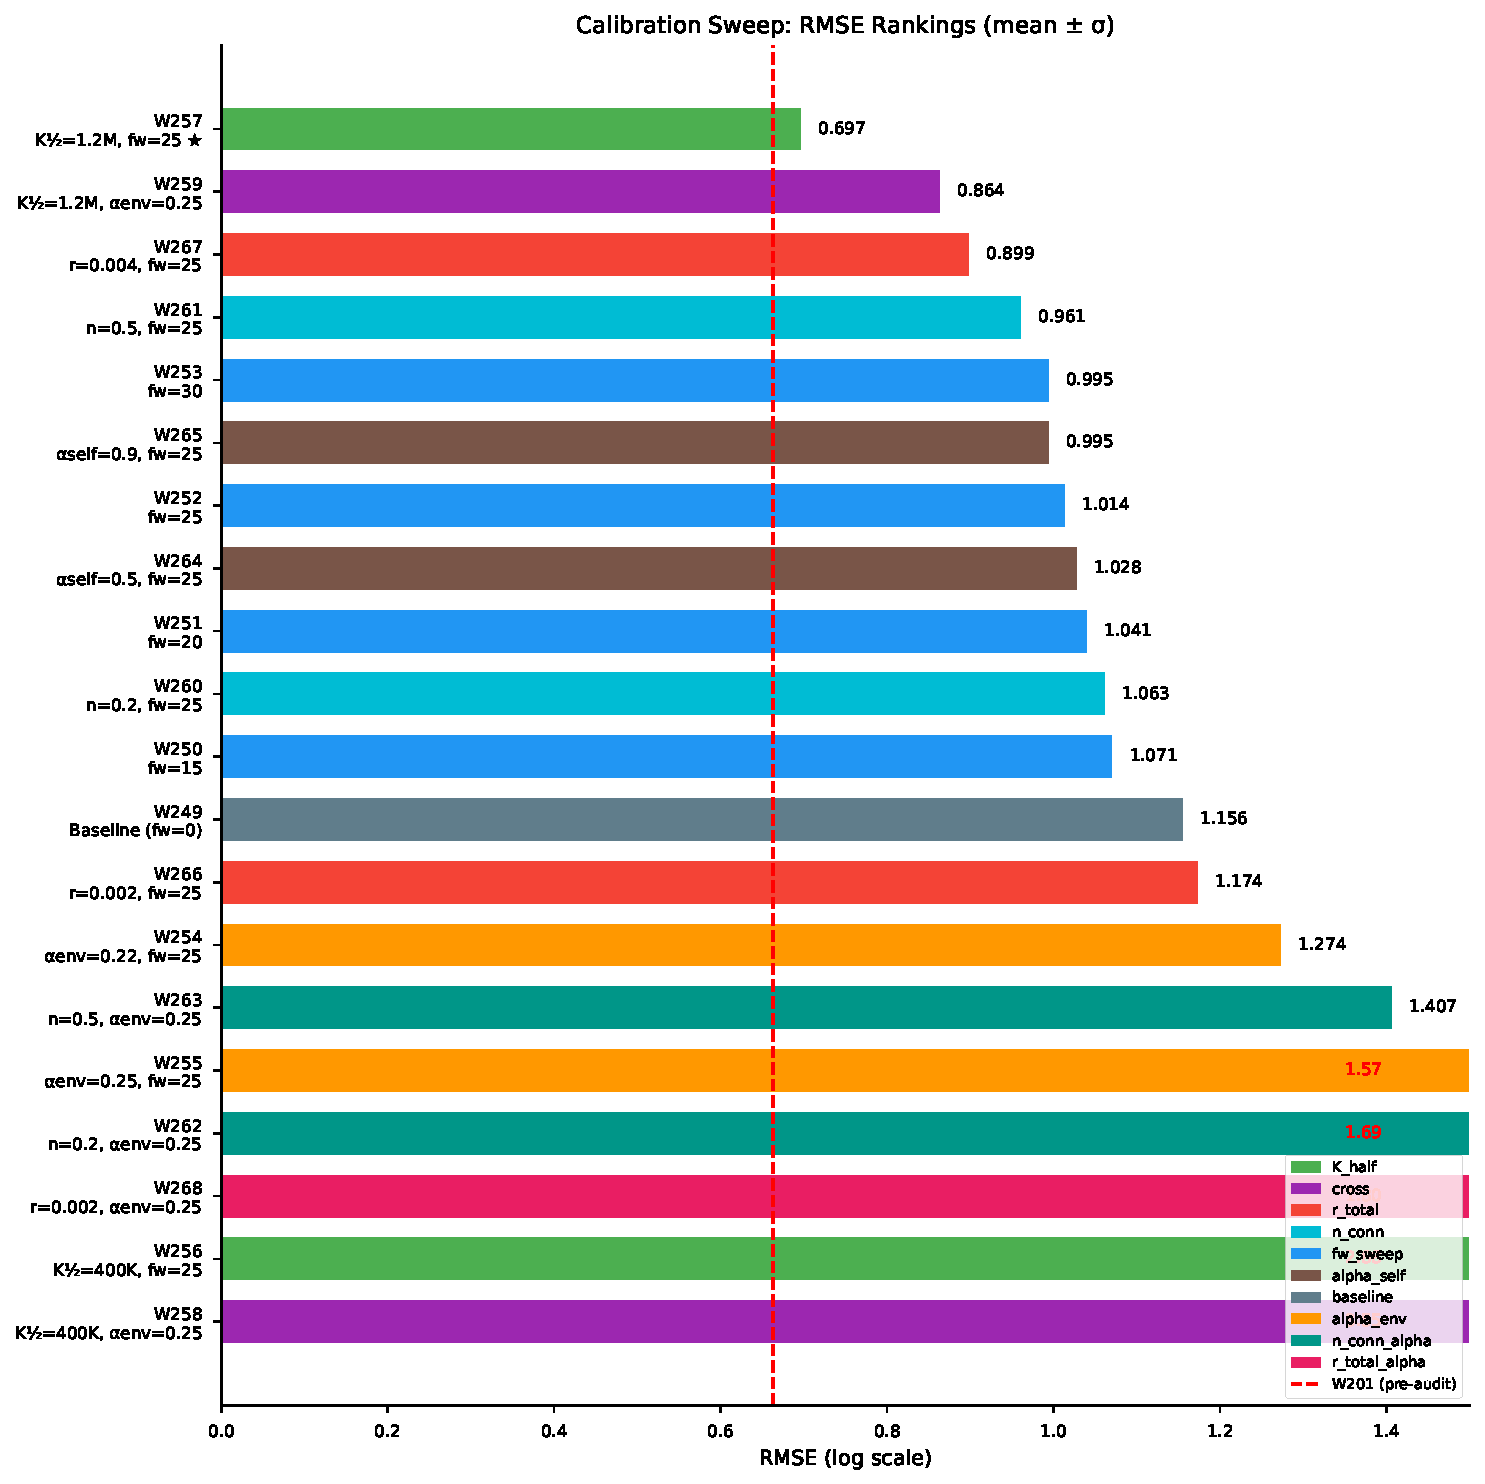
\includegraphics[width=\textwidth]{figures/fig_rmse_ranking.pdf}
\caption{\textbf{RMSE ranking for all 20 W249--W268 configurations.} Horizontal bars show mean RMSE across the 8 calibration regions; lower is better. W257 ($K_{\frac{1}{2}} = 1.2\text{M}$, $f_w = 25$) achieves the best fit at RMSE = 0.697, a 40\% improvement over the post-audit baseline W249 (RMSE = 1.156). The two $K_{\frac{1}{2}} = 400\text{K}$ configurations (W256, W258) are catastrophically poor, confirming that low $K_{\frac{1}{2}}$ suppresses recovery across all regions.}
\label{fig:rmse_ranking}
\end{figure}

\clearpage

\begin{figure}[H]
\centering
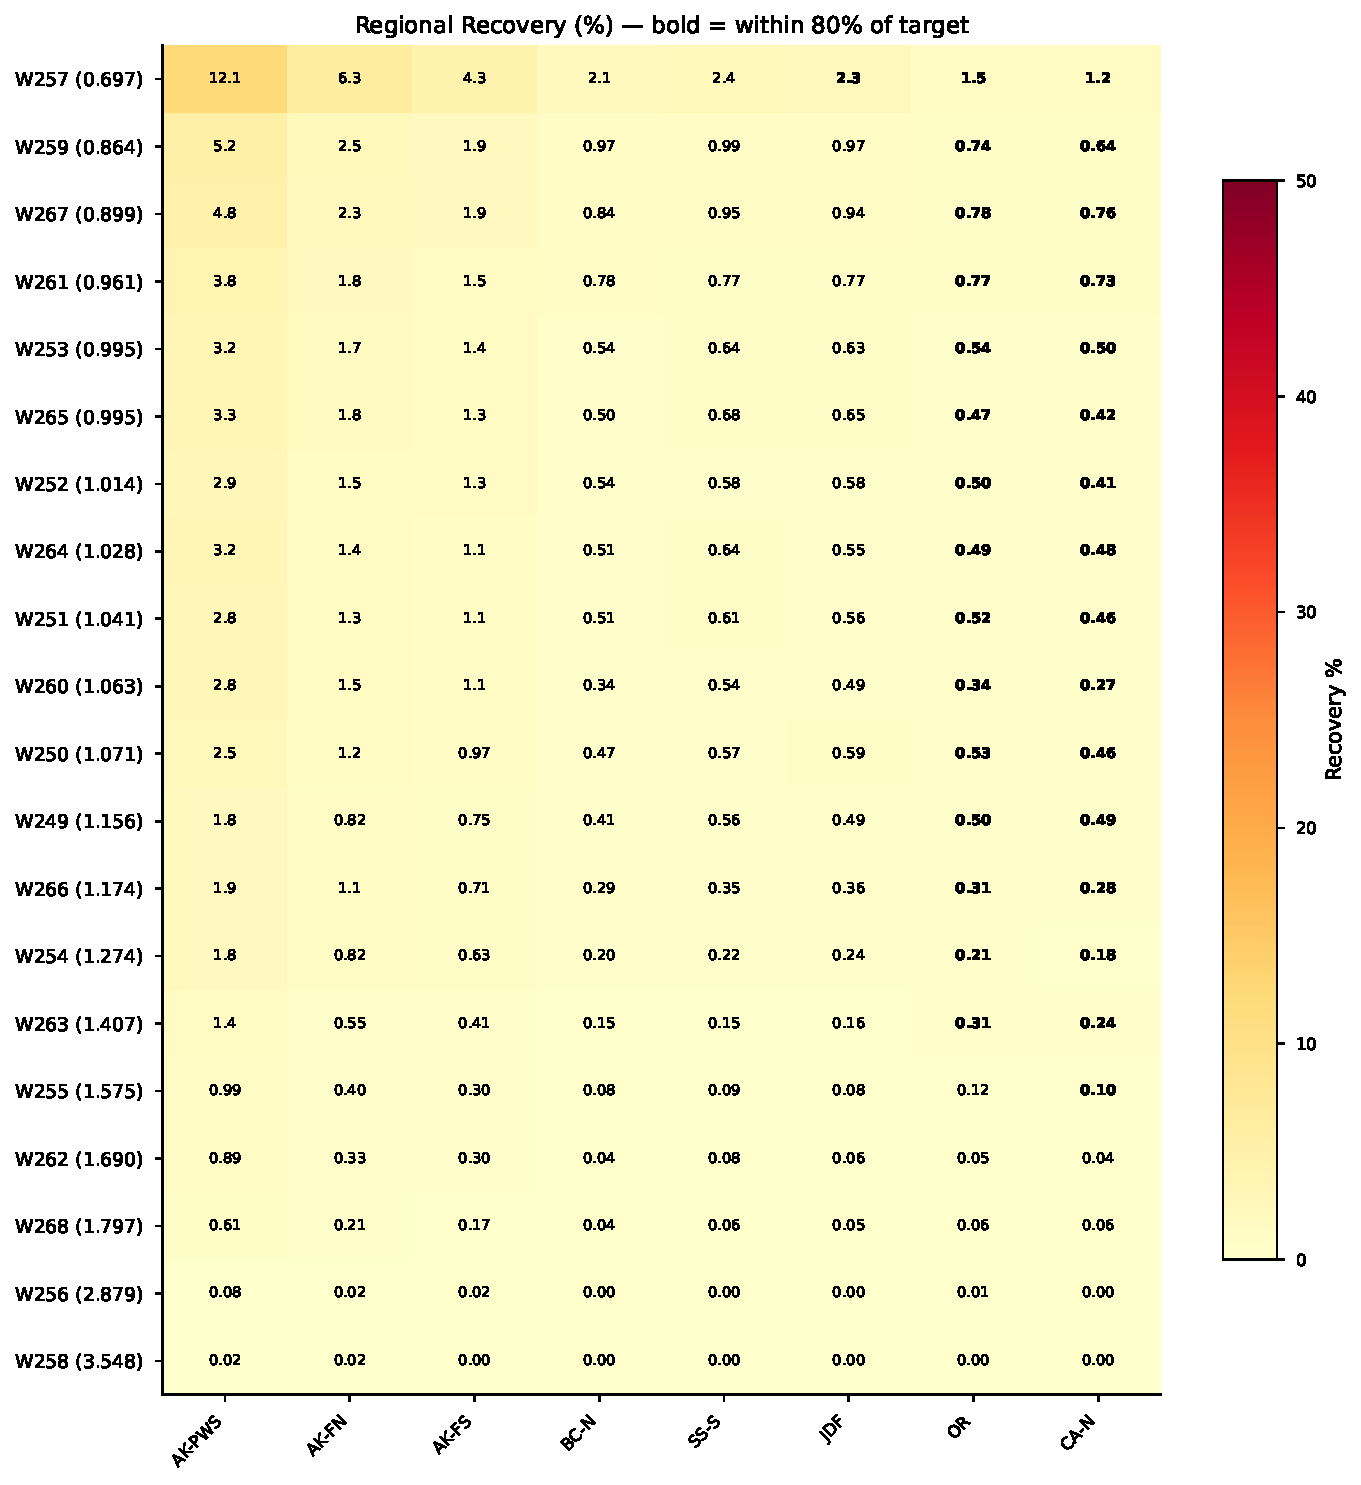
\includegraphics[width=\textwidth]{figures/fig_region_heatmap.pdf}
\caption{\textbf{Configuration $\times$ region recovery heatmap for all 20 configurations across 18 regions.} Each cell shows the recovery fraction; warmer colors indicate higher recovery. Rows are ordered by RMSE rank (W257 at top). W257 shows the strongest northern recovery (AK-PWS: 12.1\%, AK-AL: 19.7\%) while $K_{\frac{1}{2}} = 400\text{K}$ configs (W256, W258) are nearly blank. Configurations with $\alpha_{\text{env}} \geq 0.22$ (W254, W255, W262, W268) show globally suppressed recovery.}
\label{fig:region_heatmap}
\end{figure}

\clearpage

\begin{figure}[H]
\centering
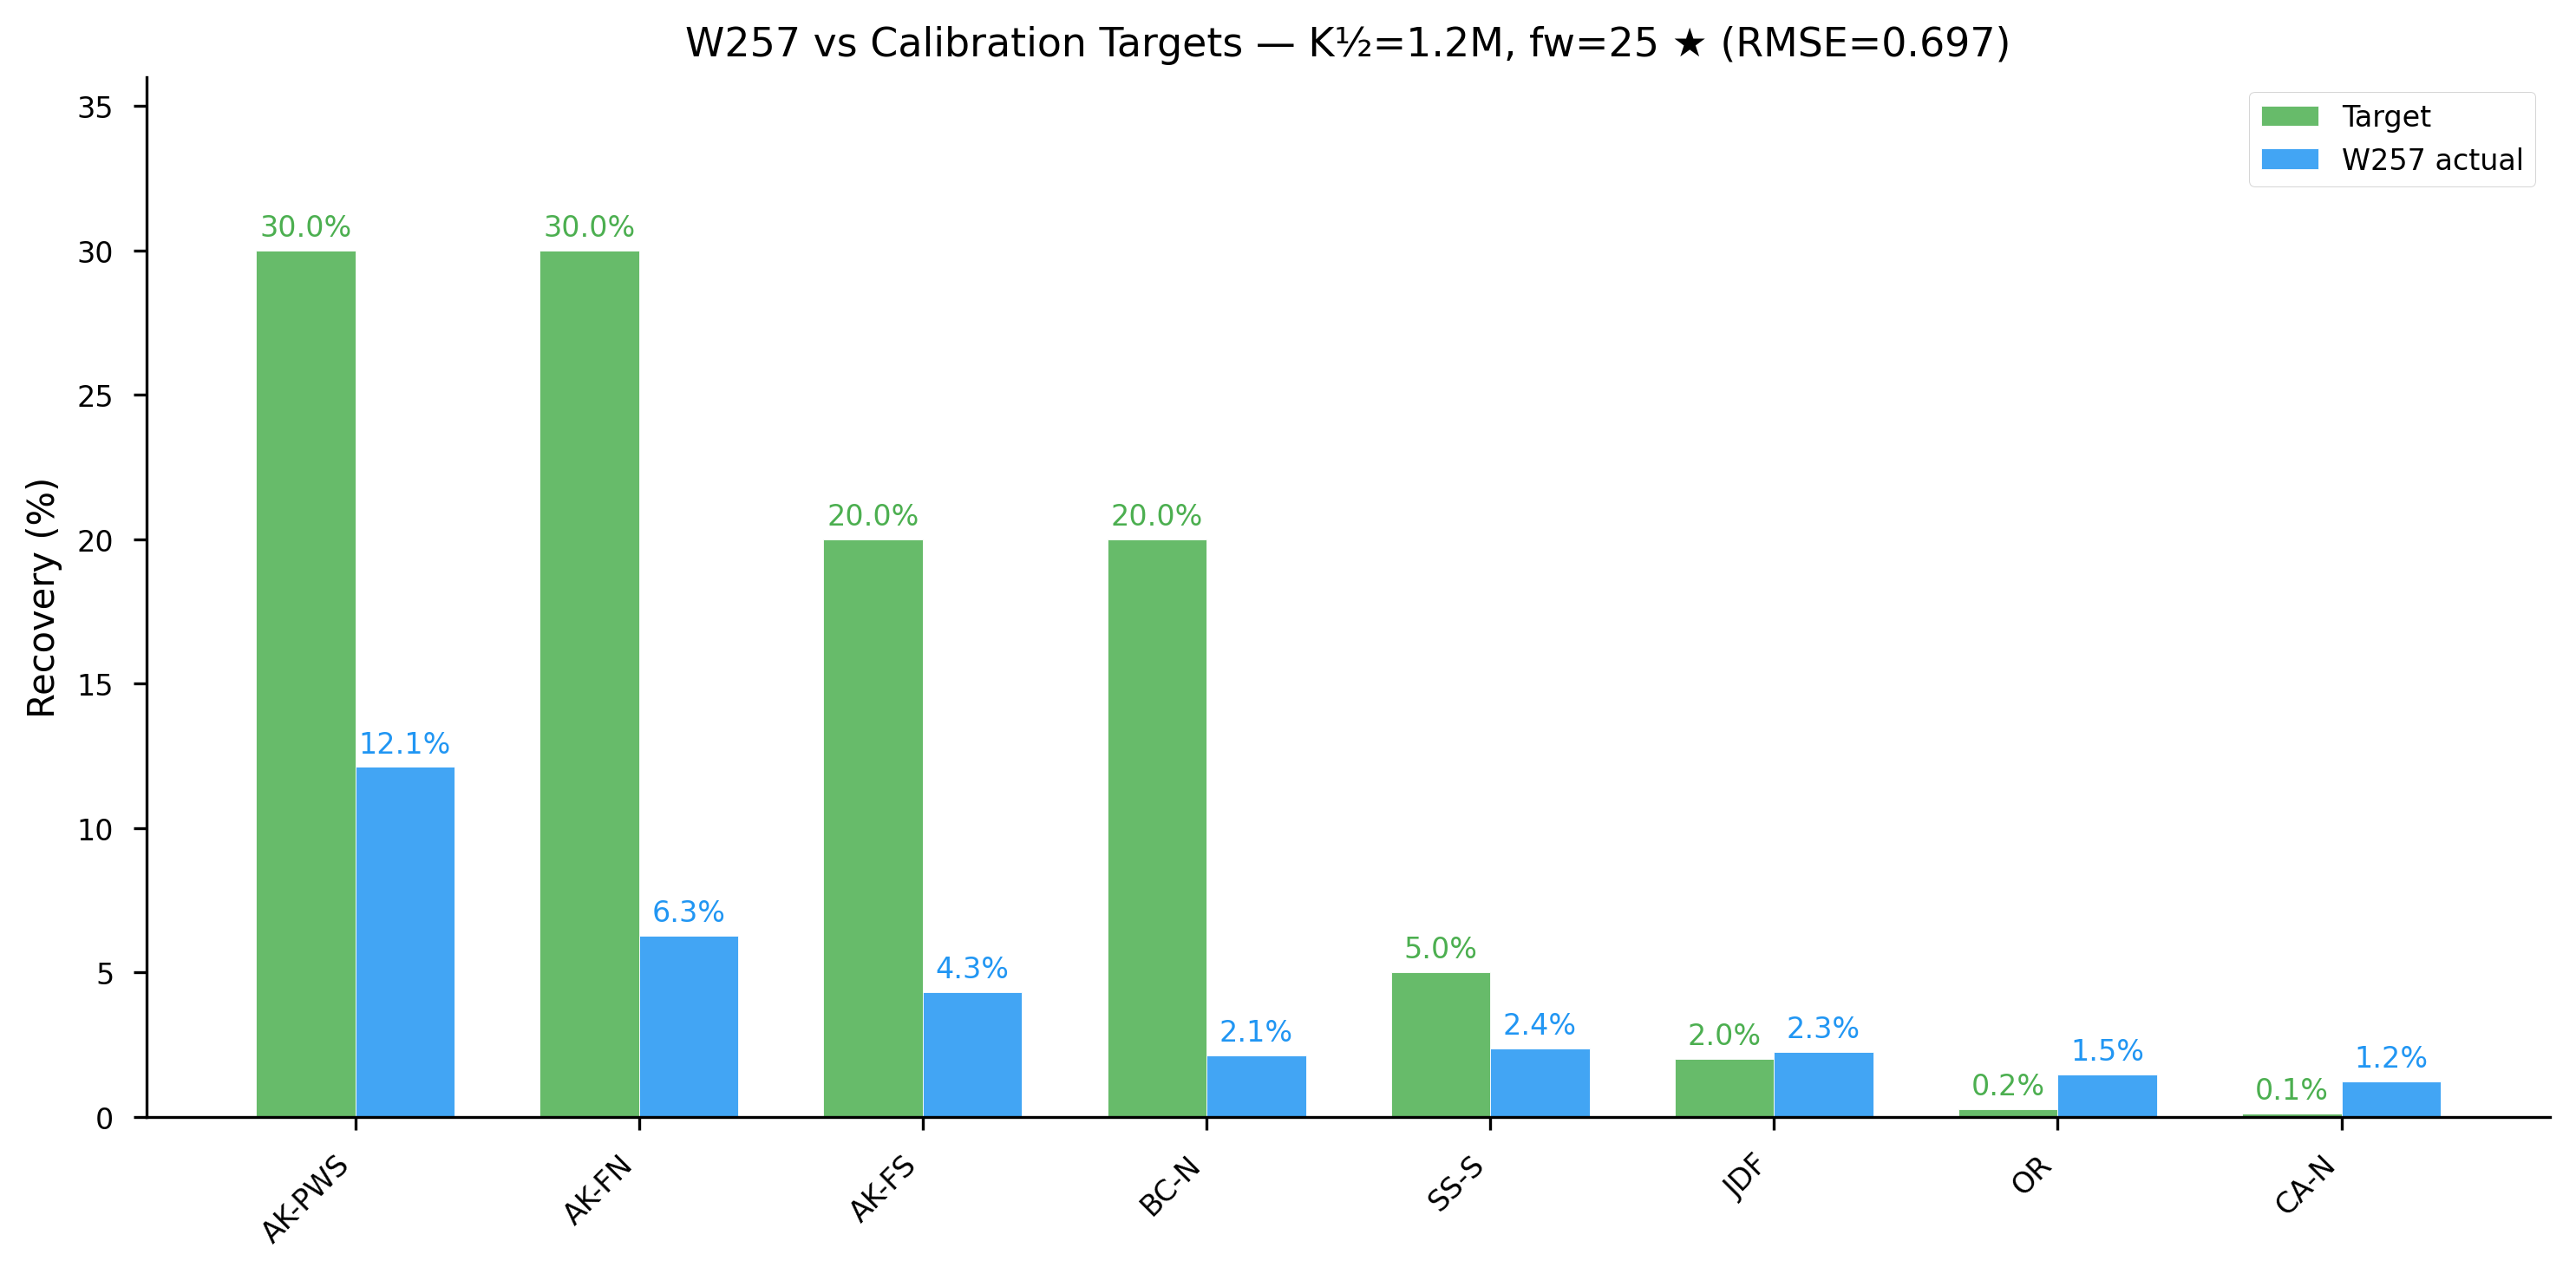
\includegraphics[width=\textwidth]{figures/fig_recovery_vs_targets.png}
\caption{\textbf{W257 recovery vs.\ 8-region calibration targets.} Grouped bars compare W257's achieved recovery (colored) against field-derived targets (gray) for each calibration region. W257 reaches 12.1\% AK-PWS recovery against the 30\% target (40\% of target), and exceeds the JDF target (2.25\% vs.\ 2.0\%). Southern regions overshoot significantly: CA-N achieves 1.22\% vs.\ the 0.1\% target ($12\times$) and OR reaches 1.45\% vs.\ the 0.25\% target ($5.8\times$).}
\label{fig:recovery_vs_targets}
\end{figure}

\clearpage

\begin{figure}[H]
\centering
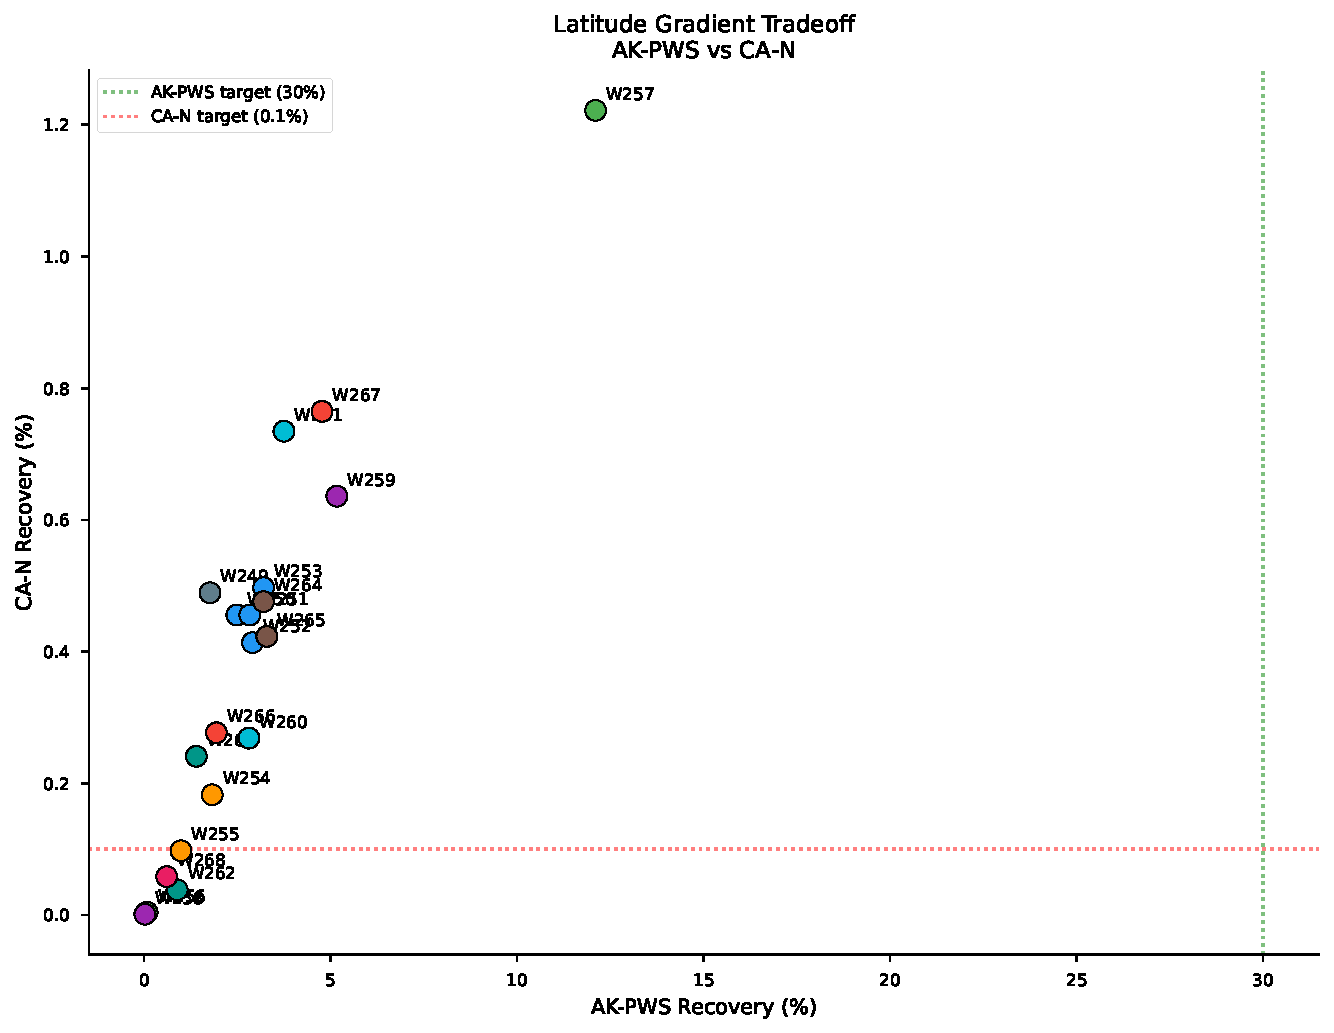
\includegraphics[width=\textwidth]{figures/fig_tradeoff.pdf}
\caption{\textbf{AK-PWS vs.\ CA-N latitude tradeoff.} Each point represents one configuration, with AK-PWS recovery on the $y$-axis and CA-N recovery on the $x$-axis. The ideal configuration would appear in the upper-left corner (high Alaska recovery, low California recovery). W257 achieves the highest AK-PWS recovery (12.1\%) but at the cost of the highest CA-N recovery (1.22\%). No configuration achieves the Pareto-optimal combination of $>$10\% AK-PWS with $<$0.5\% CA-N, confirming the latitude tradeoff as the central calibration challenge.}
\label{fig:tradeoff}
\end{figure}

\clearpage

% ══════════════════════════════════════════════════════════
% SECTION 4: SPATIAL-TEMPORAL DYNAMICS
% ══════════════════════════════════════════════════════════
\section{Spatial-Temporal Dynamics}

\sectionintro{Spatial-temporal dynamics of the best configuration (W257). These figures show how disease propagates through the 896-site network, the latitude-dependent crash and recovery pattern, and the seasonal dynamics driving population change. All visualizations use W257 monthly NPZ data ($K_{\frac{1}{2}} = 1.2\text{M}$, $f_w = 25$, RMSE = 0.697).}

\begin{figure}[H]
\centering
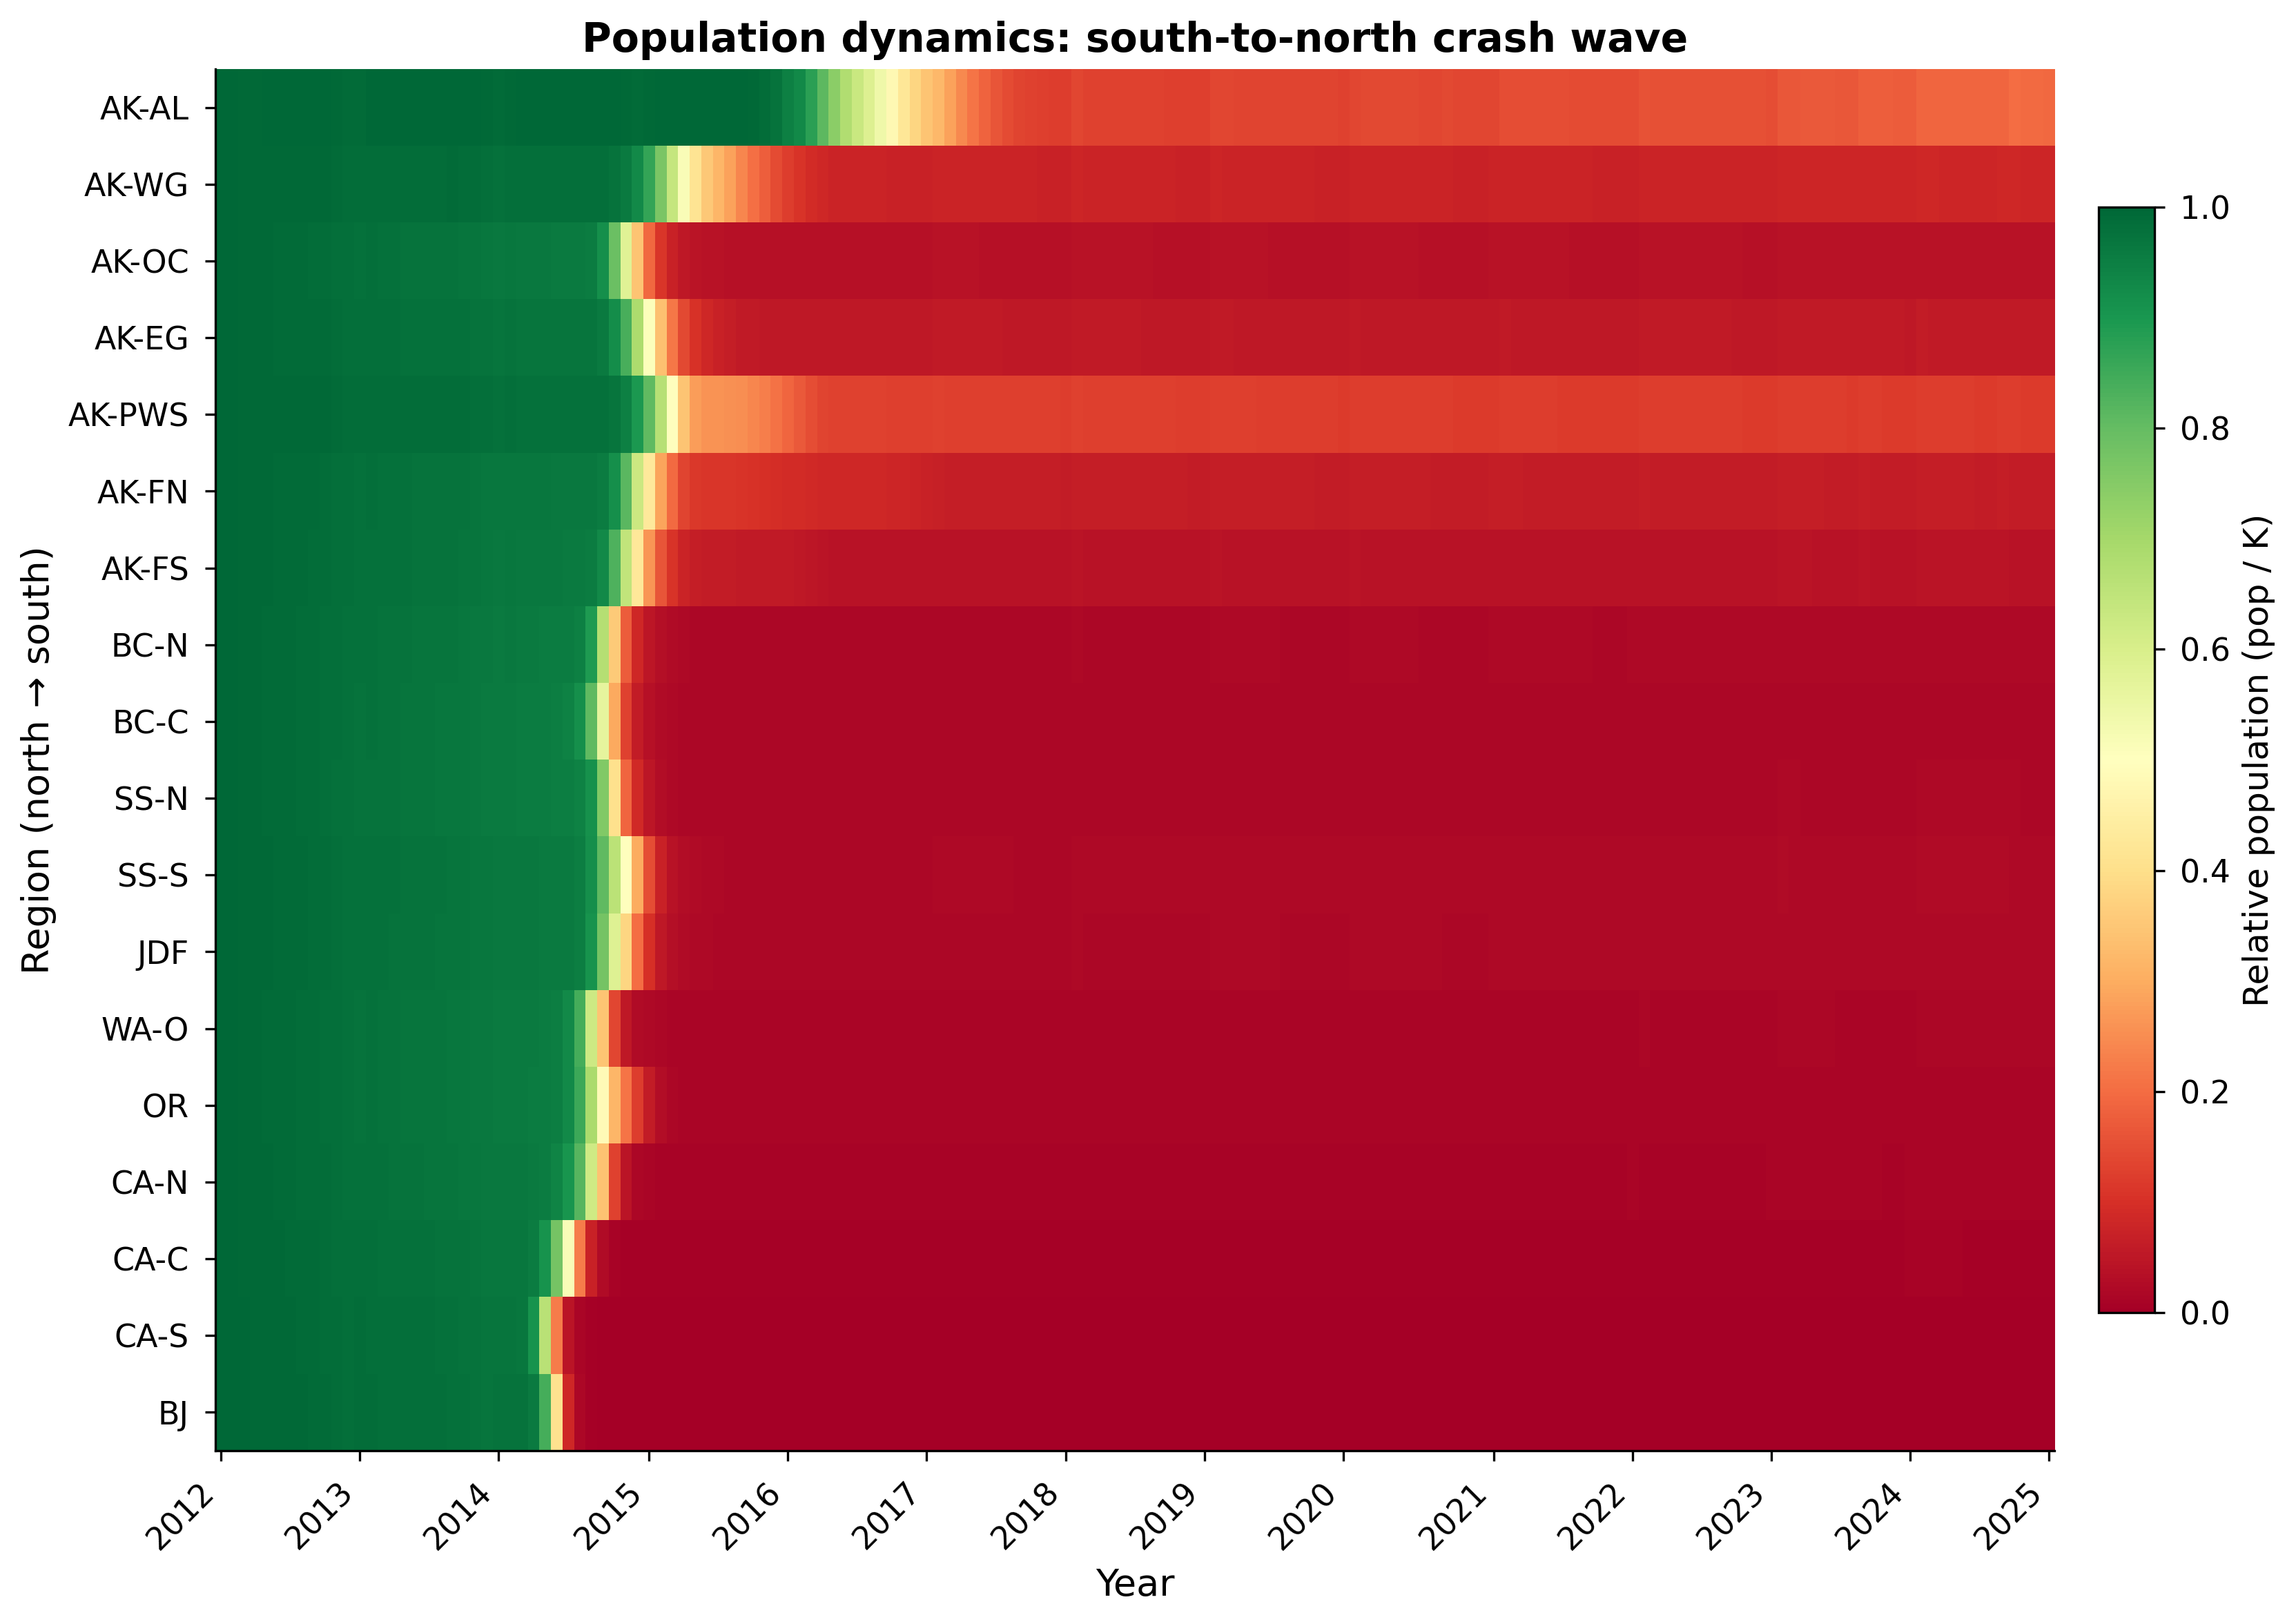
\includegraphics[width=\textwidth]{figures/fig_st_population_heatmap.png}
\caption{\textbf{Population heatmap across 18 regions over 13 simulated years (W257).} Color intensity shows relative population density (population/carrying capacity) aggregated by region, with regions ordered by latitude (north at top). The southward-to-northward crash wave is visible as the dark band propagating upward through time, with Alaska regions showing partial recovery in later years while southern regions remain near-extinct.}
\label{fig:st_population_heatmap}
\end{figure}

\clearpage

\begin{figure}[H]
\centering
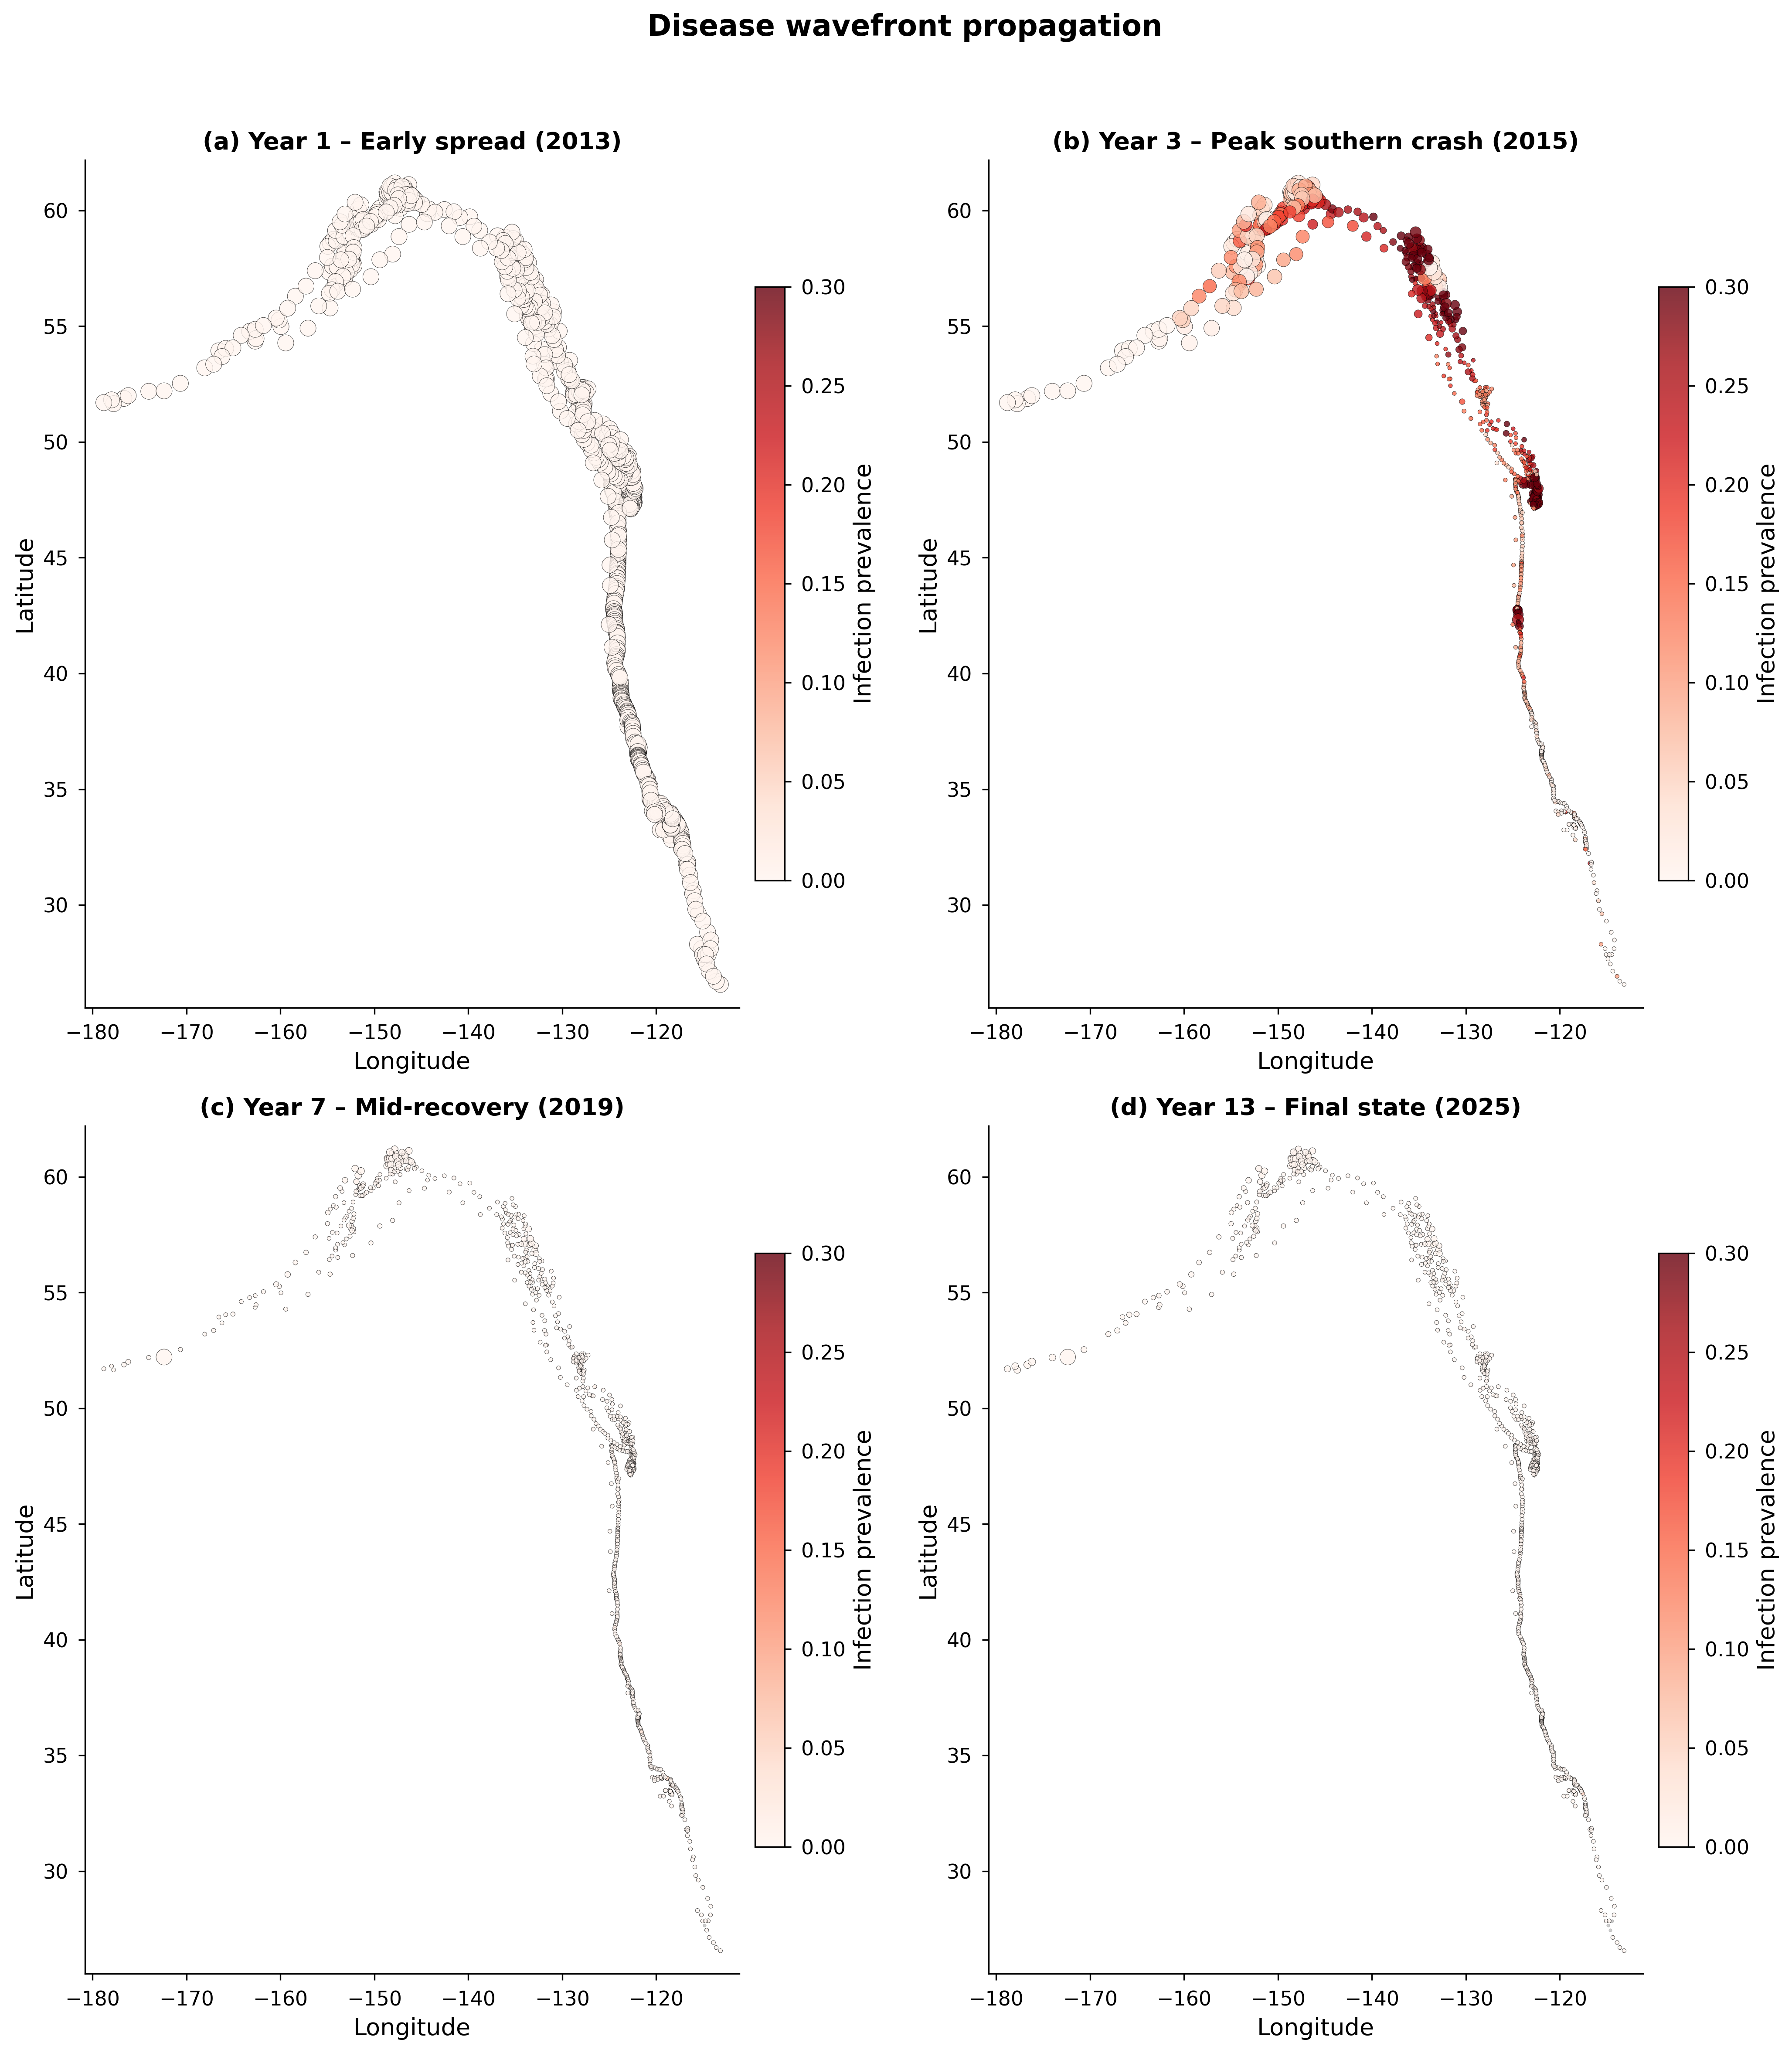
\includegraphics[width=\textwidth]{figures/fig_st_wavefront_snapshots.png}
\caption{\textbf{Disease wavefront propagation at four timepoints.} Geographic scatter of all 896 sites at years 1, 3, 7, and 13. Point color indicates infection prevalence (infected/total population); point size scales with population. Gray dots indicate extinct sites. The wavefront originates at the Channel Islands (bottom) and propagates northward, reaching Alaska by year 3. By year 13, infection persists at low prevalence across the range.}
\label{fig:st_wavefront_snapshots}
\end{figure}

\clearpage

\begin{figure}[H]
\centering
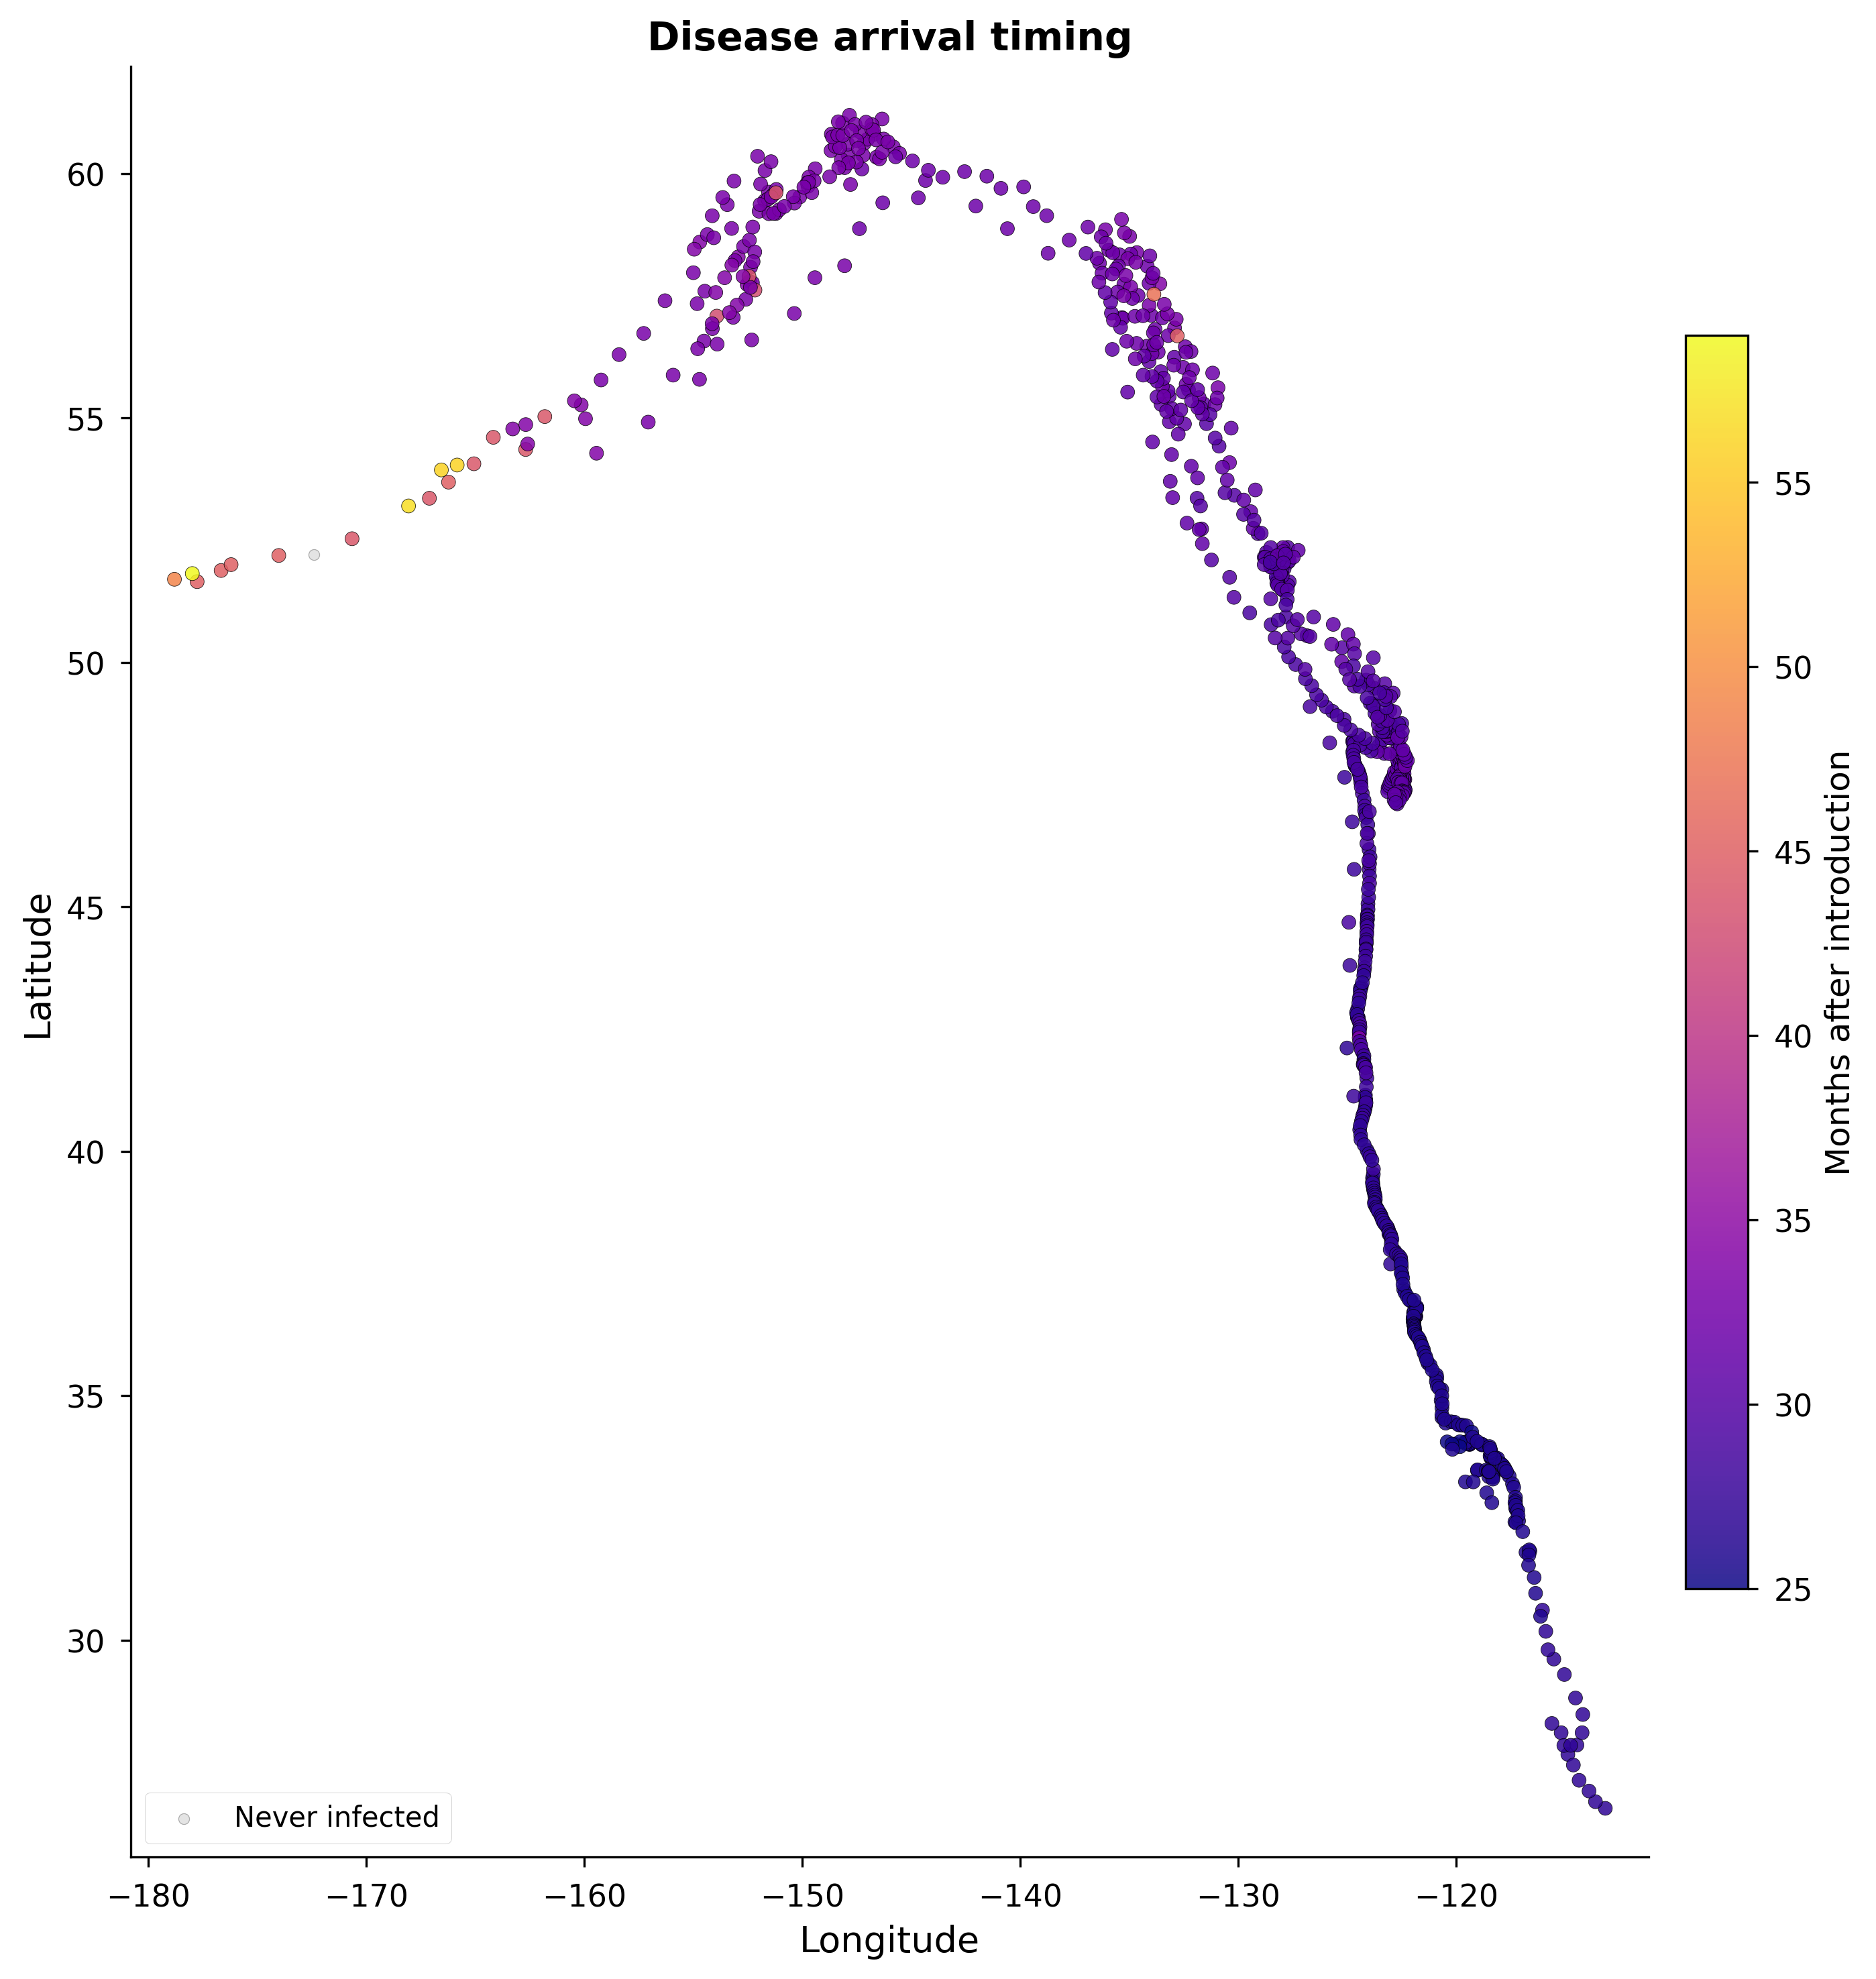
\includegraphics[width=\textwidth]{figures/fig_st_arrival_timing.png}
\caption{\textbf{Disease arrival timing across the 896-site network.} Each point represents one site, colored by the month when infection first appears. Southern sites near the Channel Islands origin nodes are infected within months; the wavefront reaches Alaska 18--24 months later. Gray points indicate sites that were never directly infected. The arrival pattern validates the wavefront propagation mechanism.}
\label{fig:st_arrival_timing}
\end{figure}

\clearpage

\begin{figure}[H]
\centering
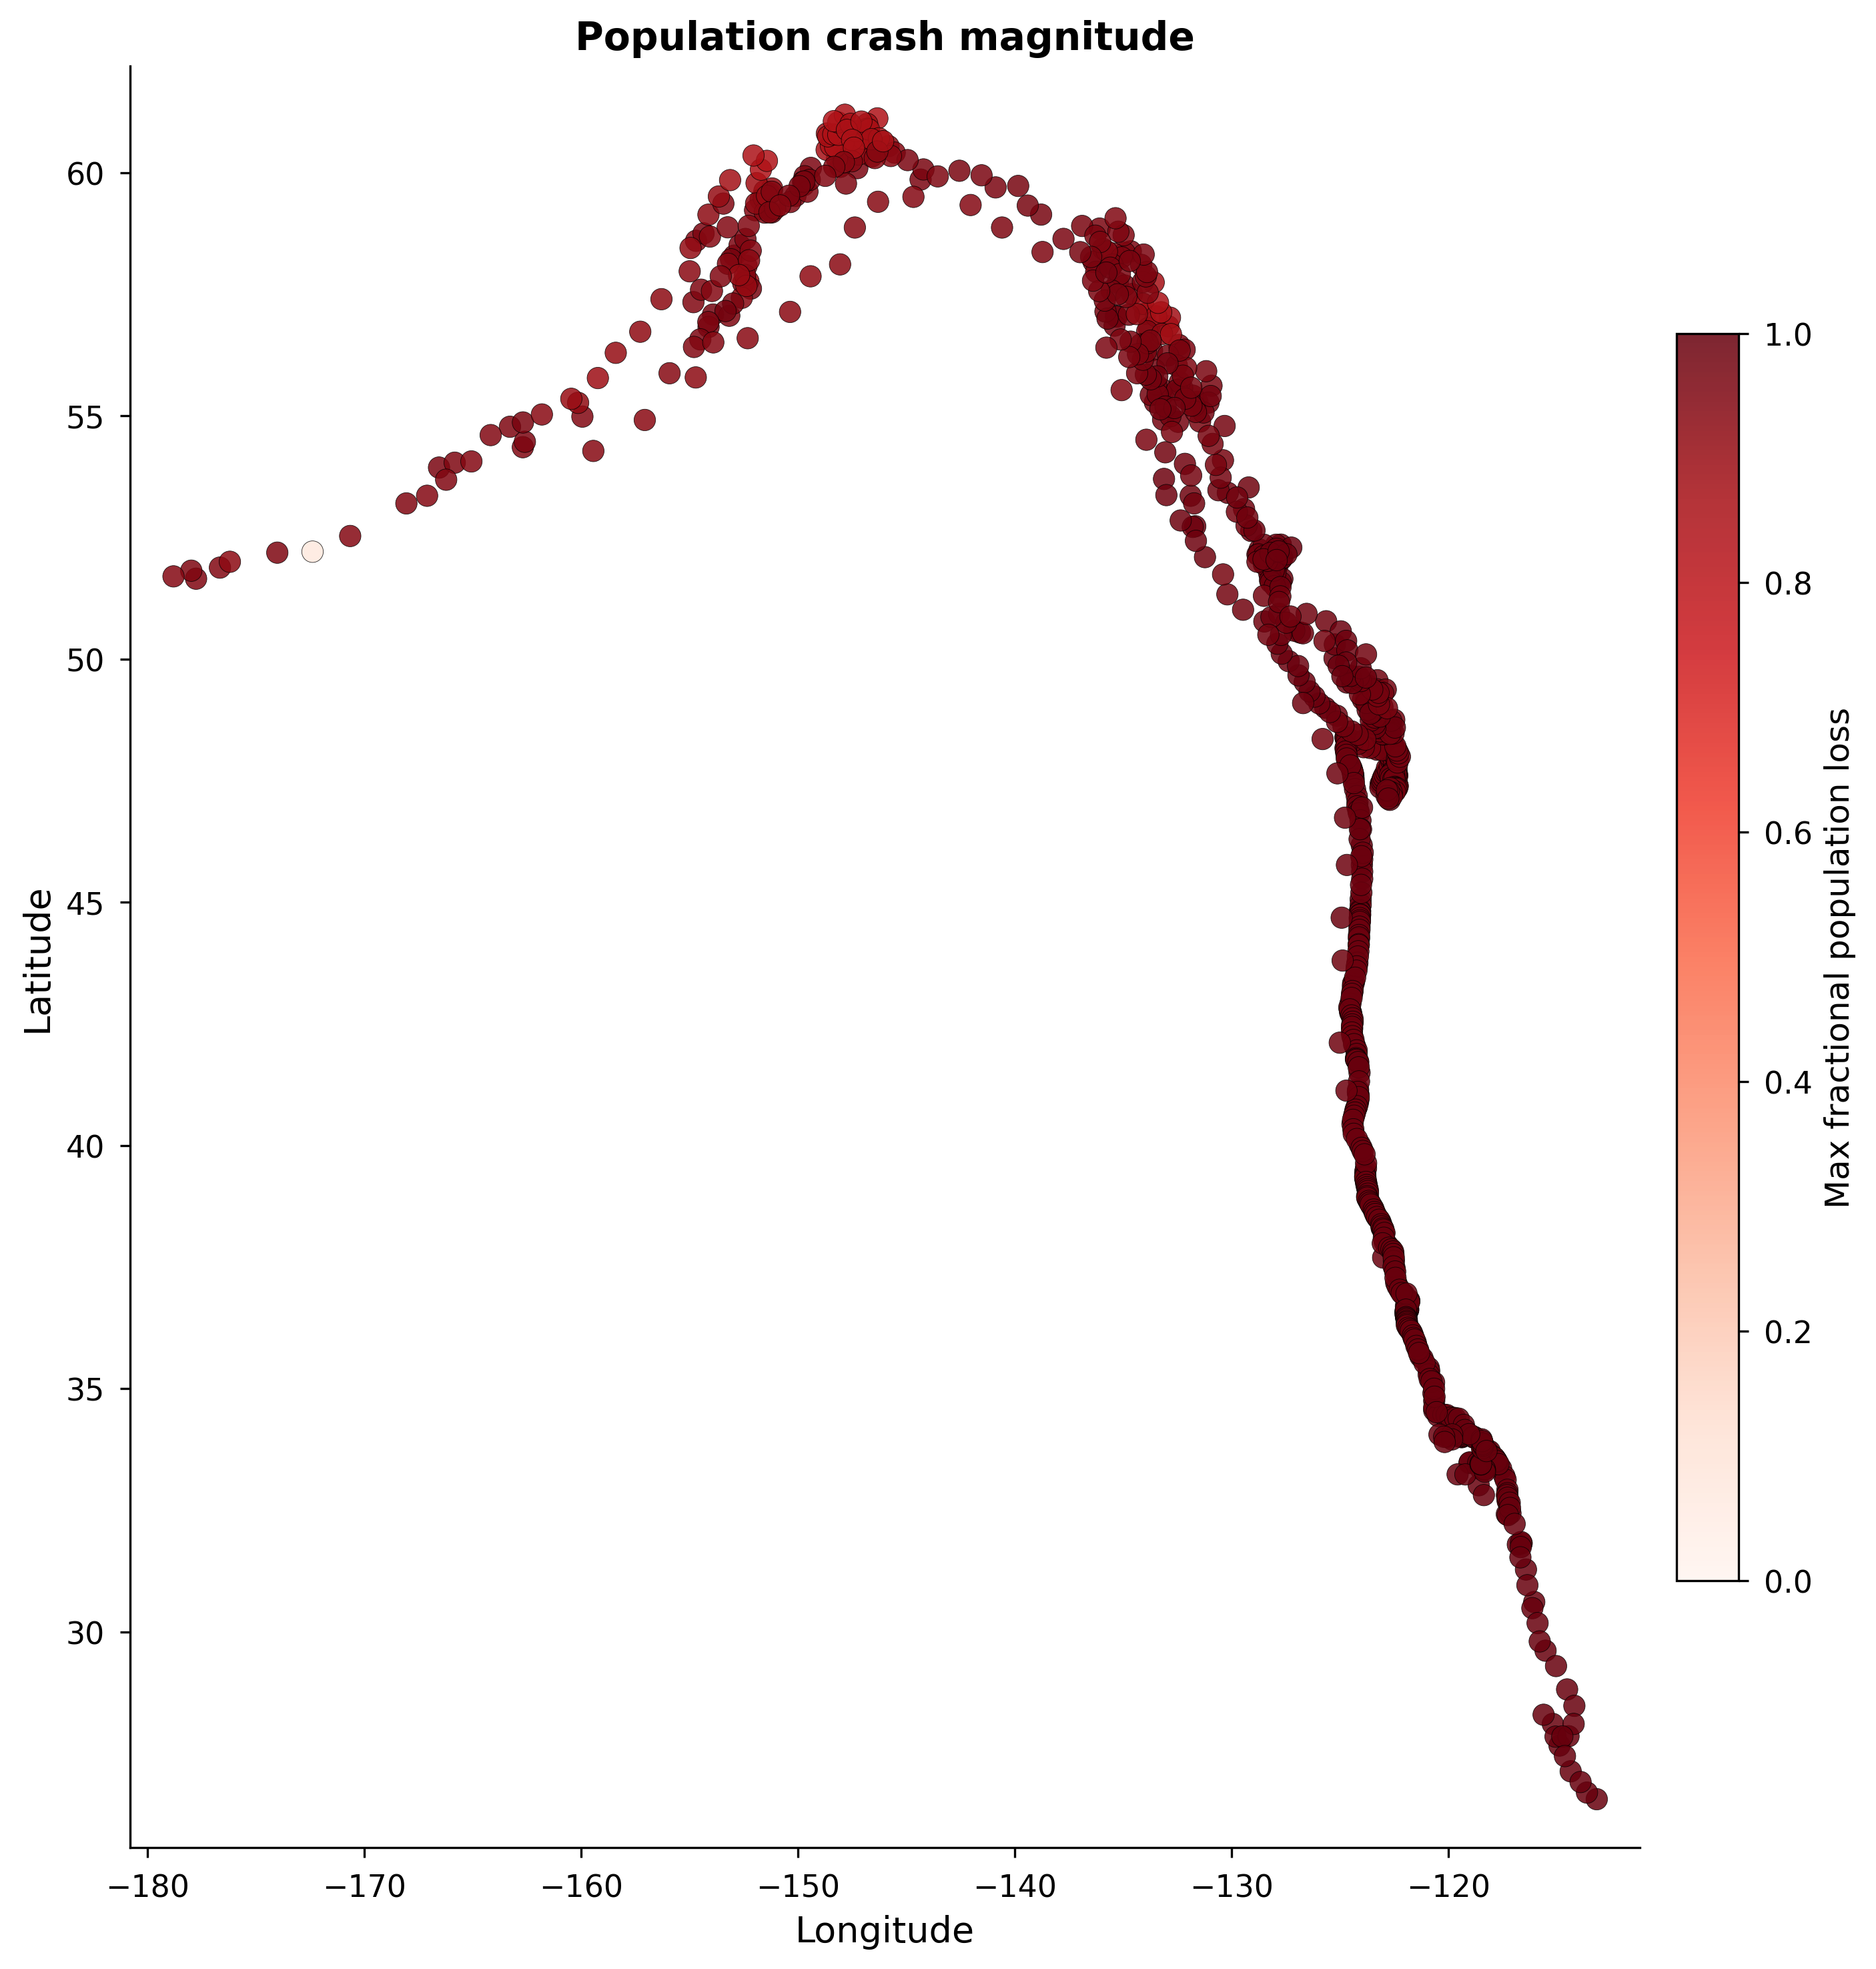
\includegraphics[width=\textwidth]{figures/fig_st_crash_magnitude.png}
\caption{\textbf{Maximum population crash magnitude by site.} Color shows the maximum fractional population loss at each site (1 minus minimum population divided by initial population). Nearly all sites experience catastrophic decline ($>$95\%), consistent with observed 90.6\% range-wide decline (Gravem et al.\ 2021). Point size scales with initial population.}
\label{fig:st_crash_magnitude}
\end{figure}

\clearpage

\begin{figure}[H]
\centering
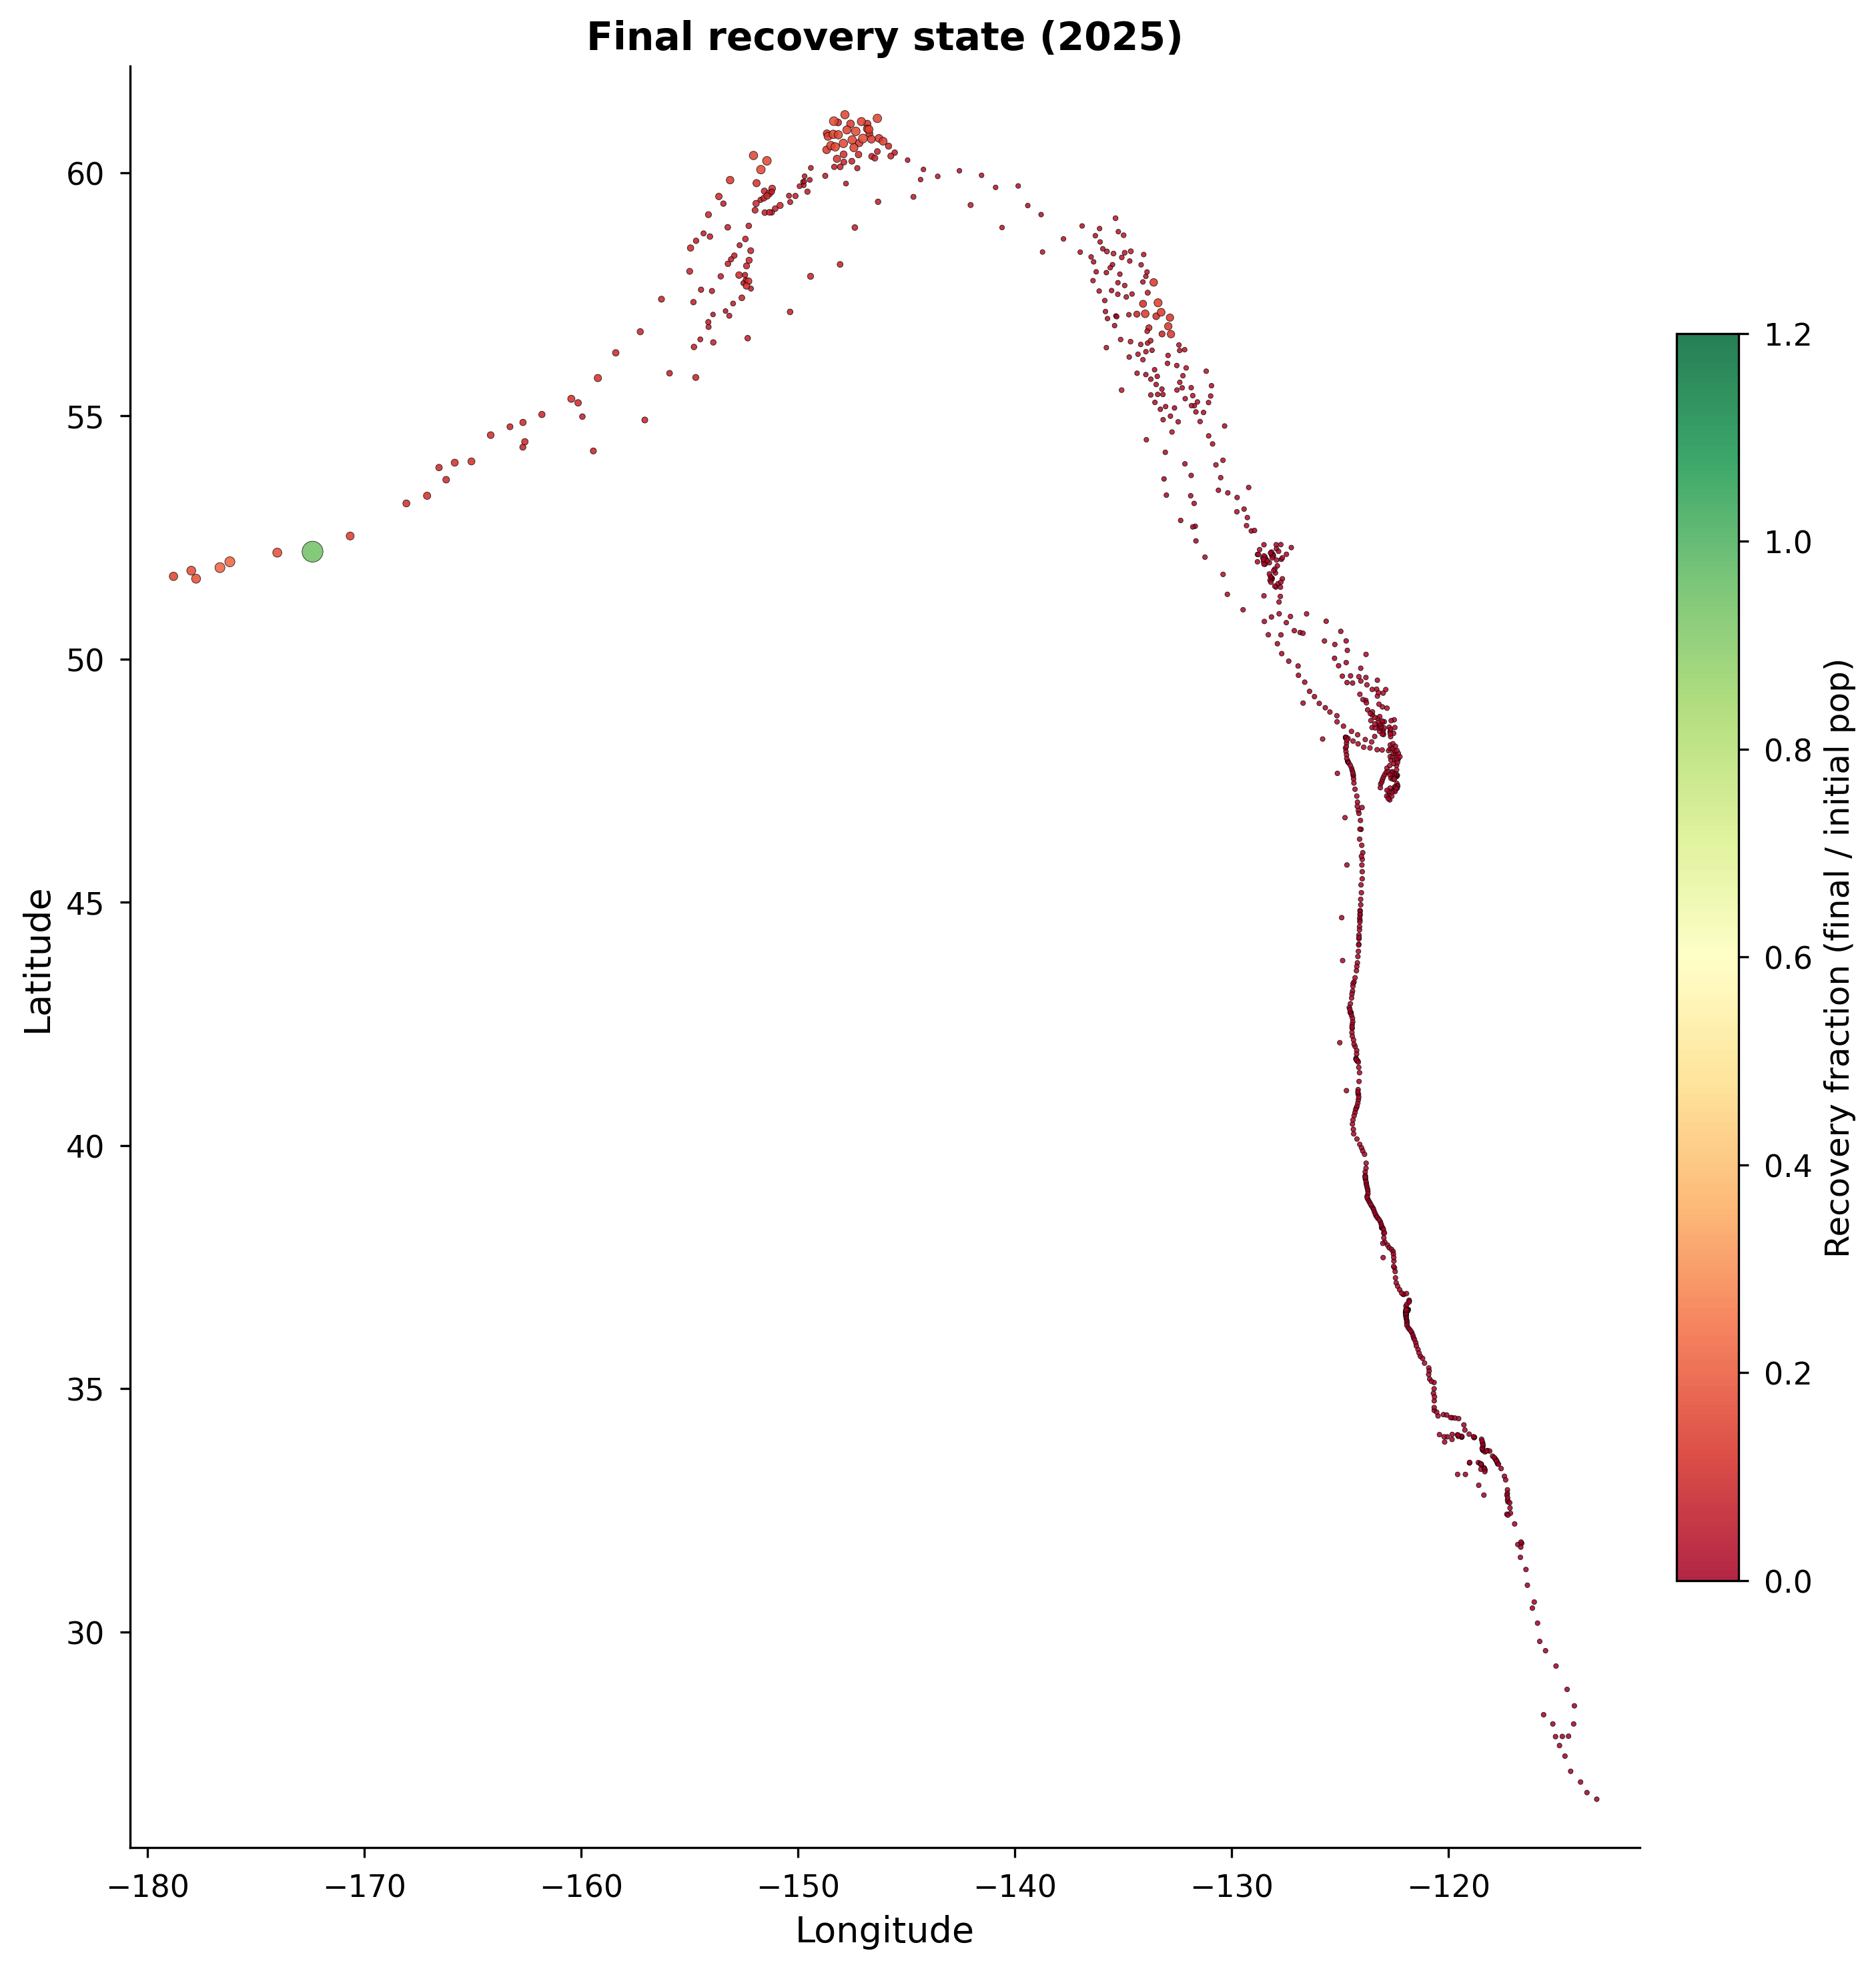
\includegraphics[width=\textwidth]{figures/fig_st_recovery_map.png}
\caption{\textbf{Final recovery state across the 896-site network (year 13).} Color shows final population as a fraction of initial population. Green indicates meaningful recovery; red indicates near-extinction. The clear latitudinal gradient --- Alaska sites recovering while California sites remain depleted --- is the model's key spatial prediction and matches observed patterns.}
\label{fig:st_recovery_map}
\end{figure}

\clearpage

\begin{figure}[H]
\centering
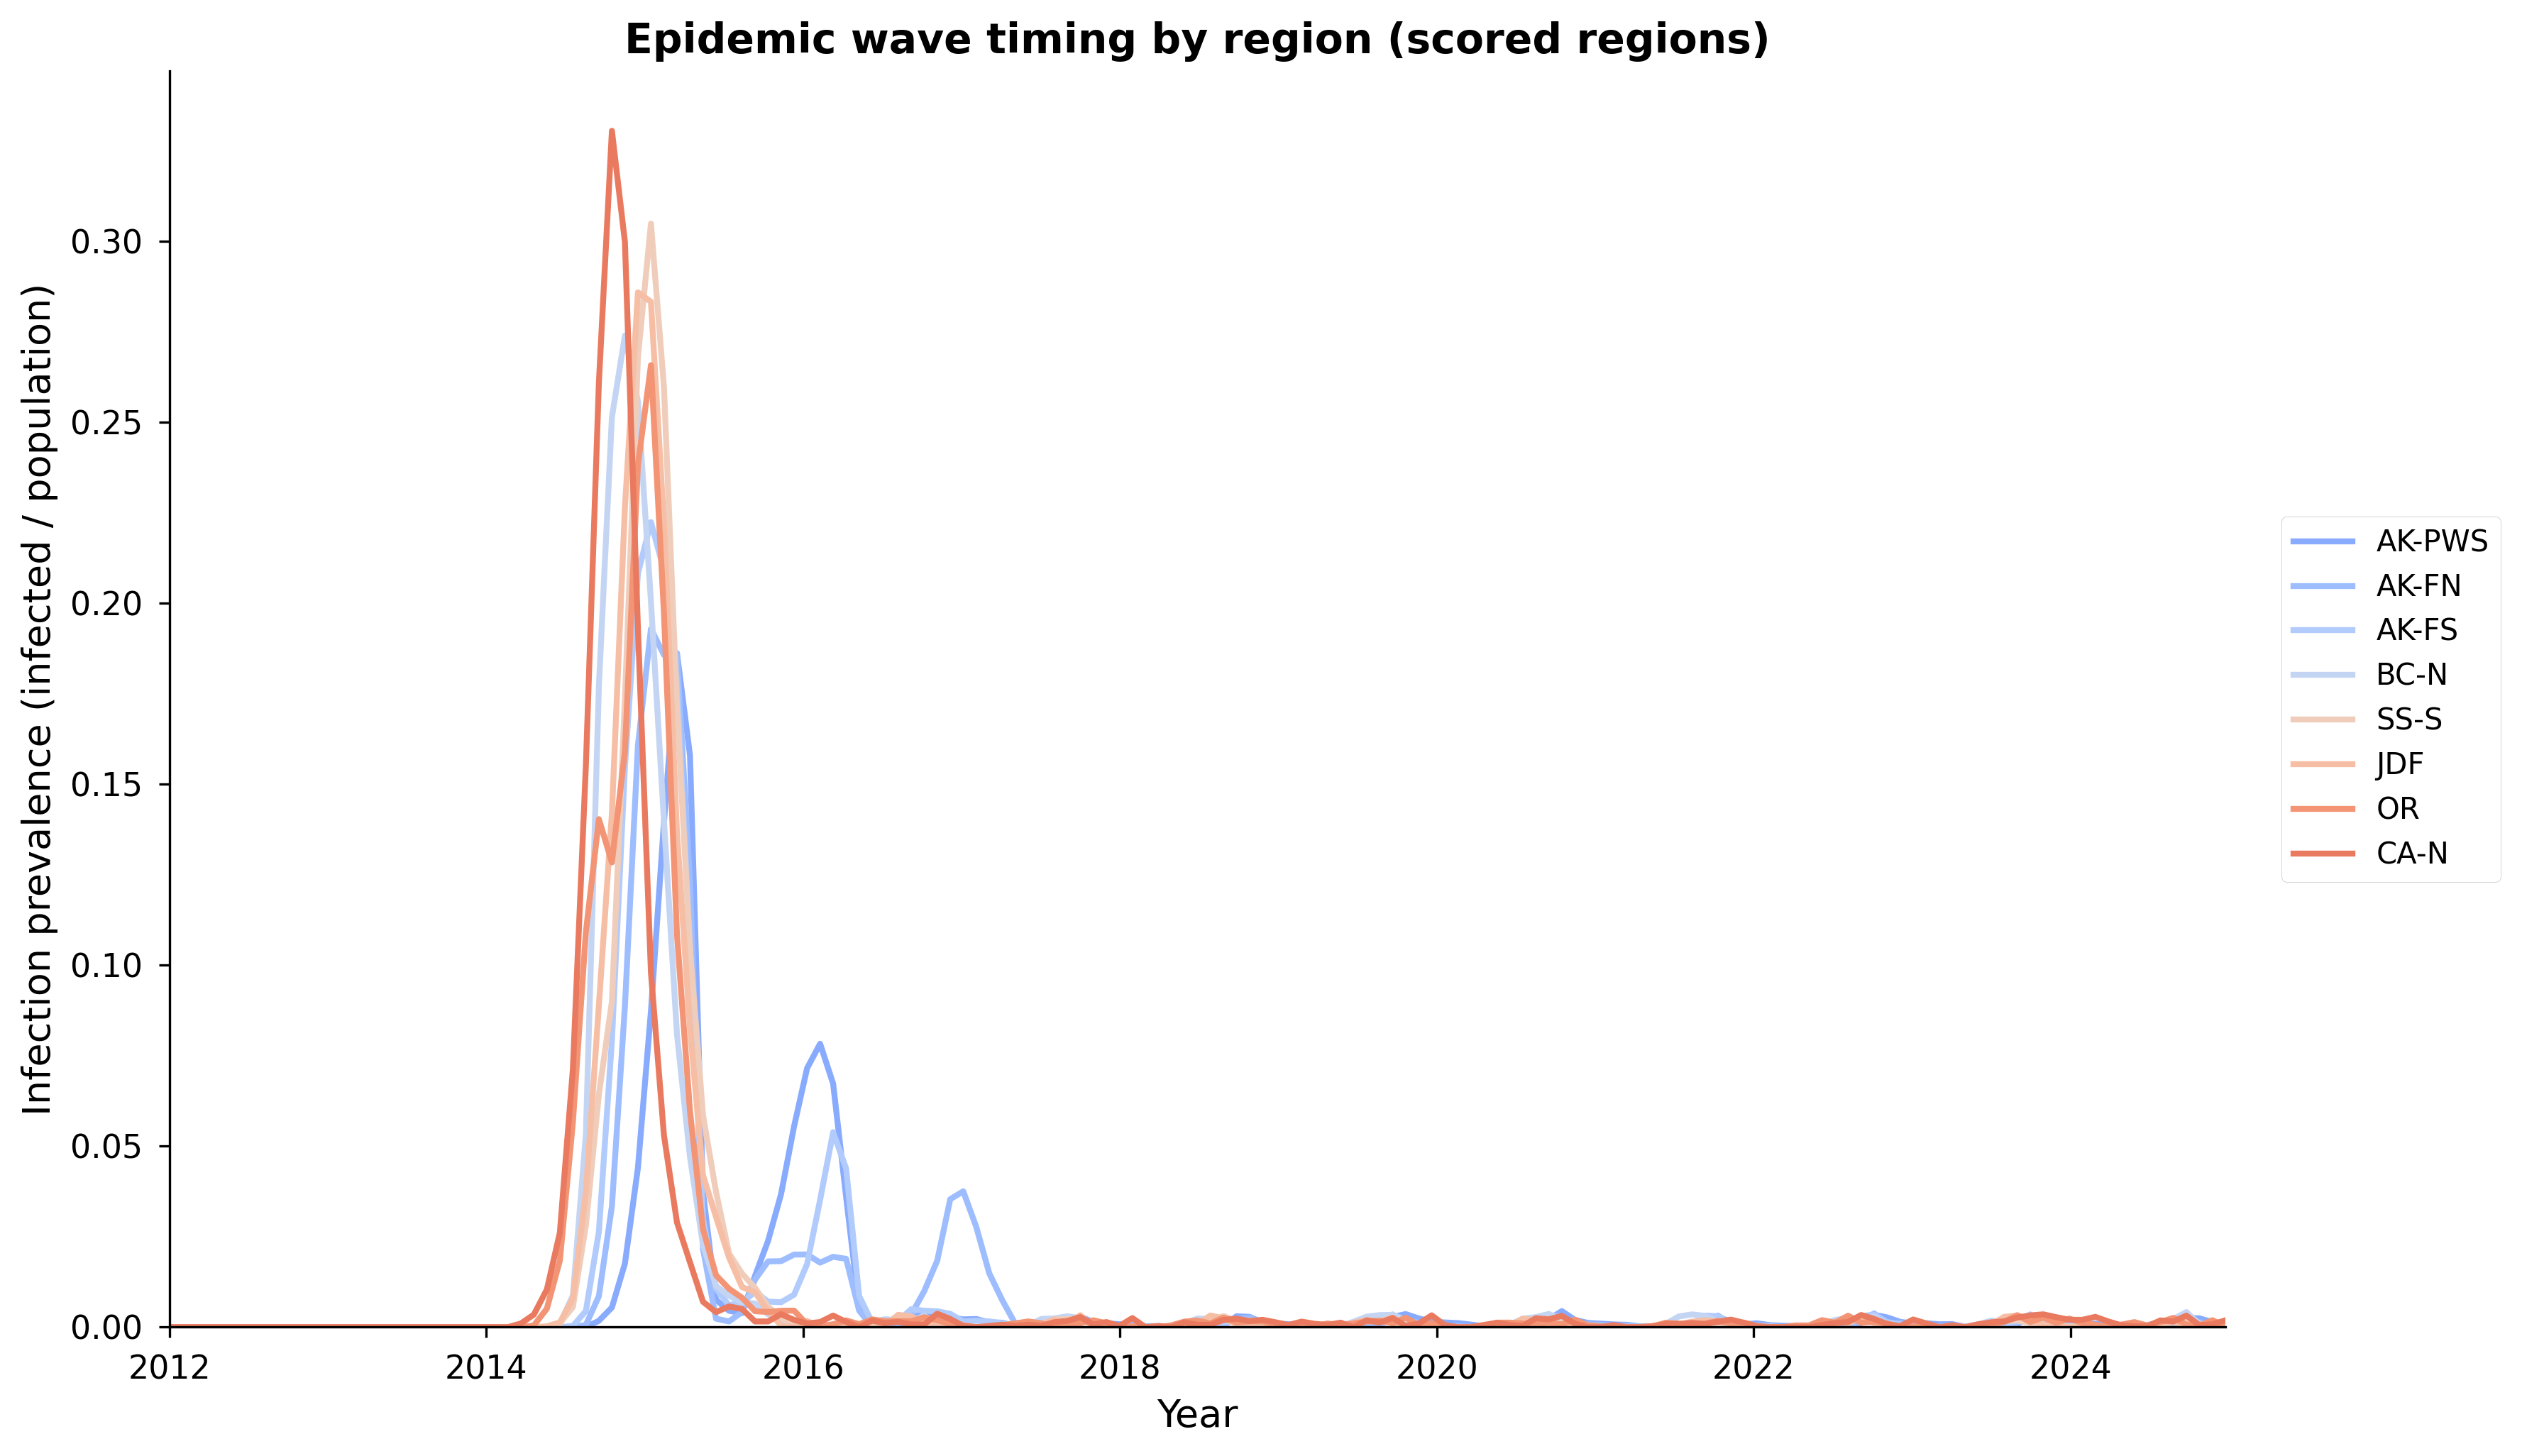
\includegraphics[width=\textwidth]{figures/fig_st_prevalence_curves.png}
\caption{\textbf{Infection prevalence time series by region.} Lines show the fraction of population infected (infected/total) for each of the 8 scored calibration regions. Southern regions (warm colors) experience earlier and sharper epidemic peaks, while northern regions (cool colors) show delayed onset. The staggered timing reflects the wavefront propagation from the Channel Islands origin.}
\label{fig:st_prevalence_curves}
\end{figure}

\clearpage

\begin{figure}[H]
\centering
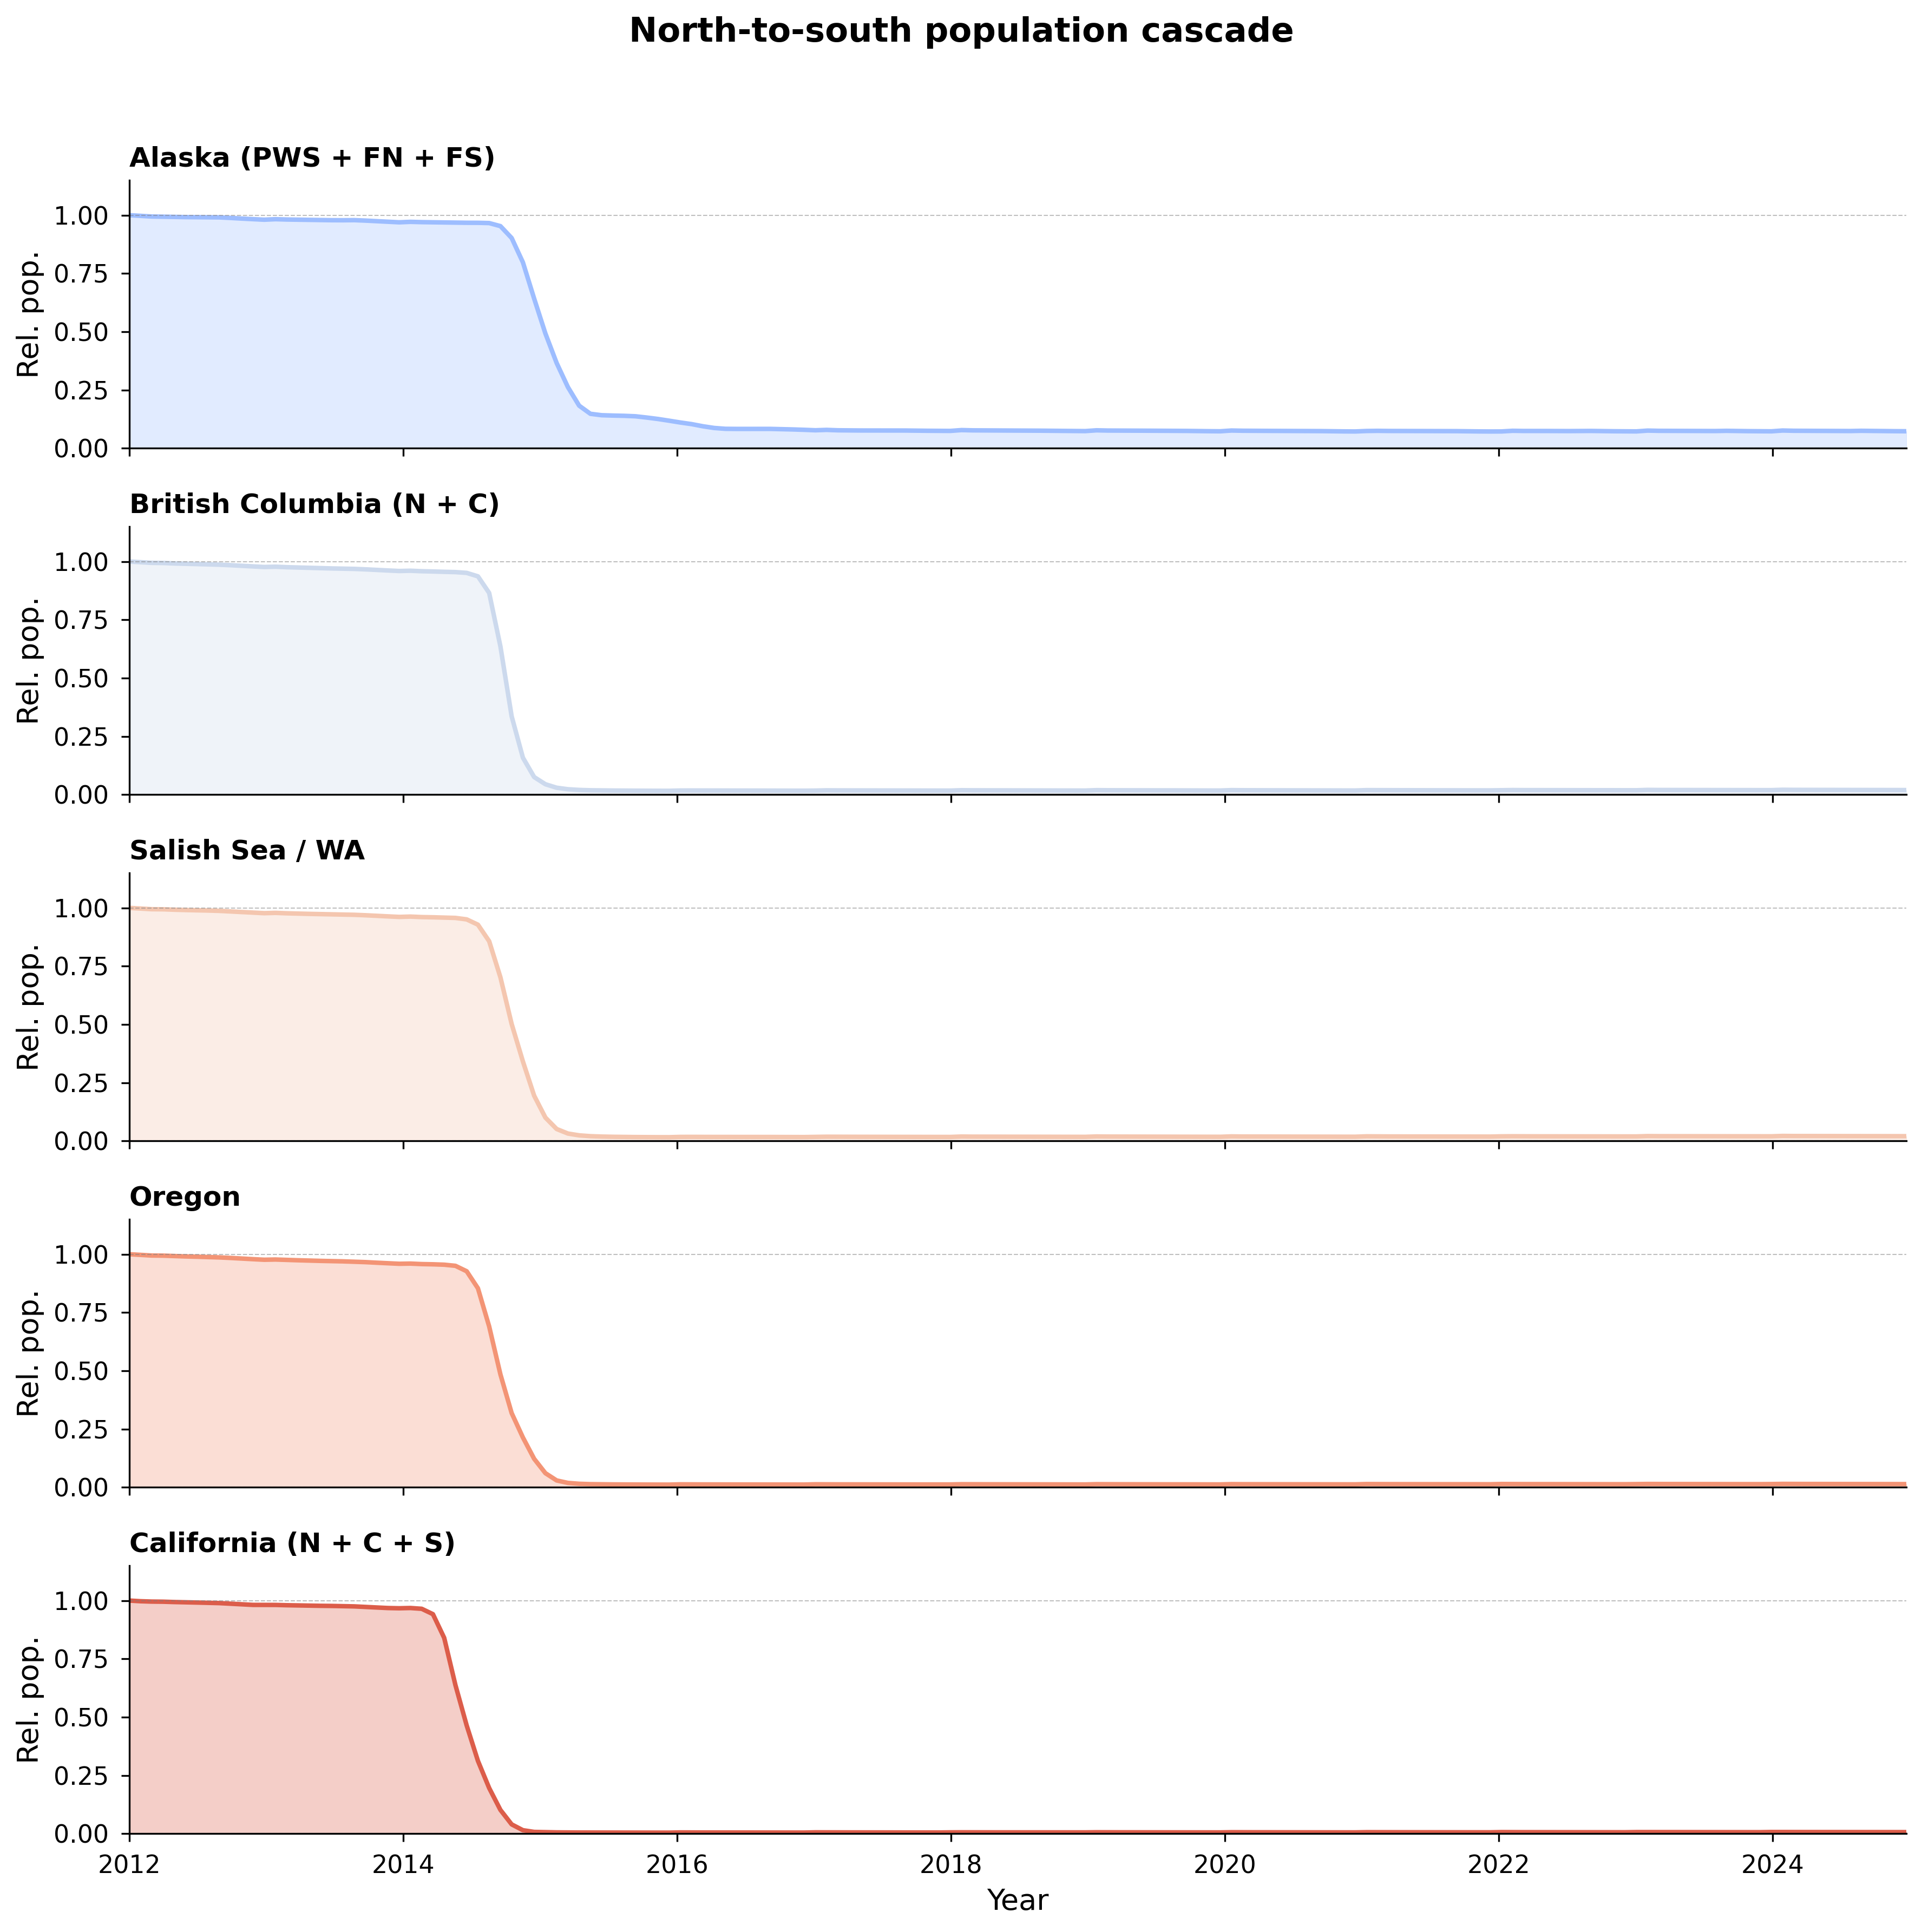
\includegraphics[width=\textwidth]{figures/fig_st_cascade_panels.png}
\caption{\textbf{North--south population cascade.} Five panels showing relative population trajectories for latitude bands: Alaska (AK-PWS, AK-FN, AK-FS), British Columbia, Salish Sea/Washington, Oregon, and California. The crash propagates from south to north with a 1--2 year delay. Recovery magnitude decreases monotonically with decreasing latitude, reproducing the observed gradient from partial northern recovery to near-total southern extirpation.}
\label{fig:st_cascade_panels}
\end{figure}

\clearpage

\begin{figure}[H]
\centering
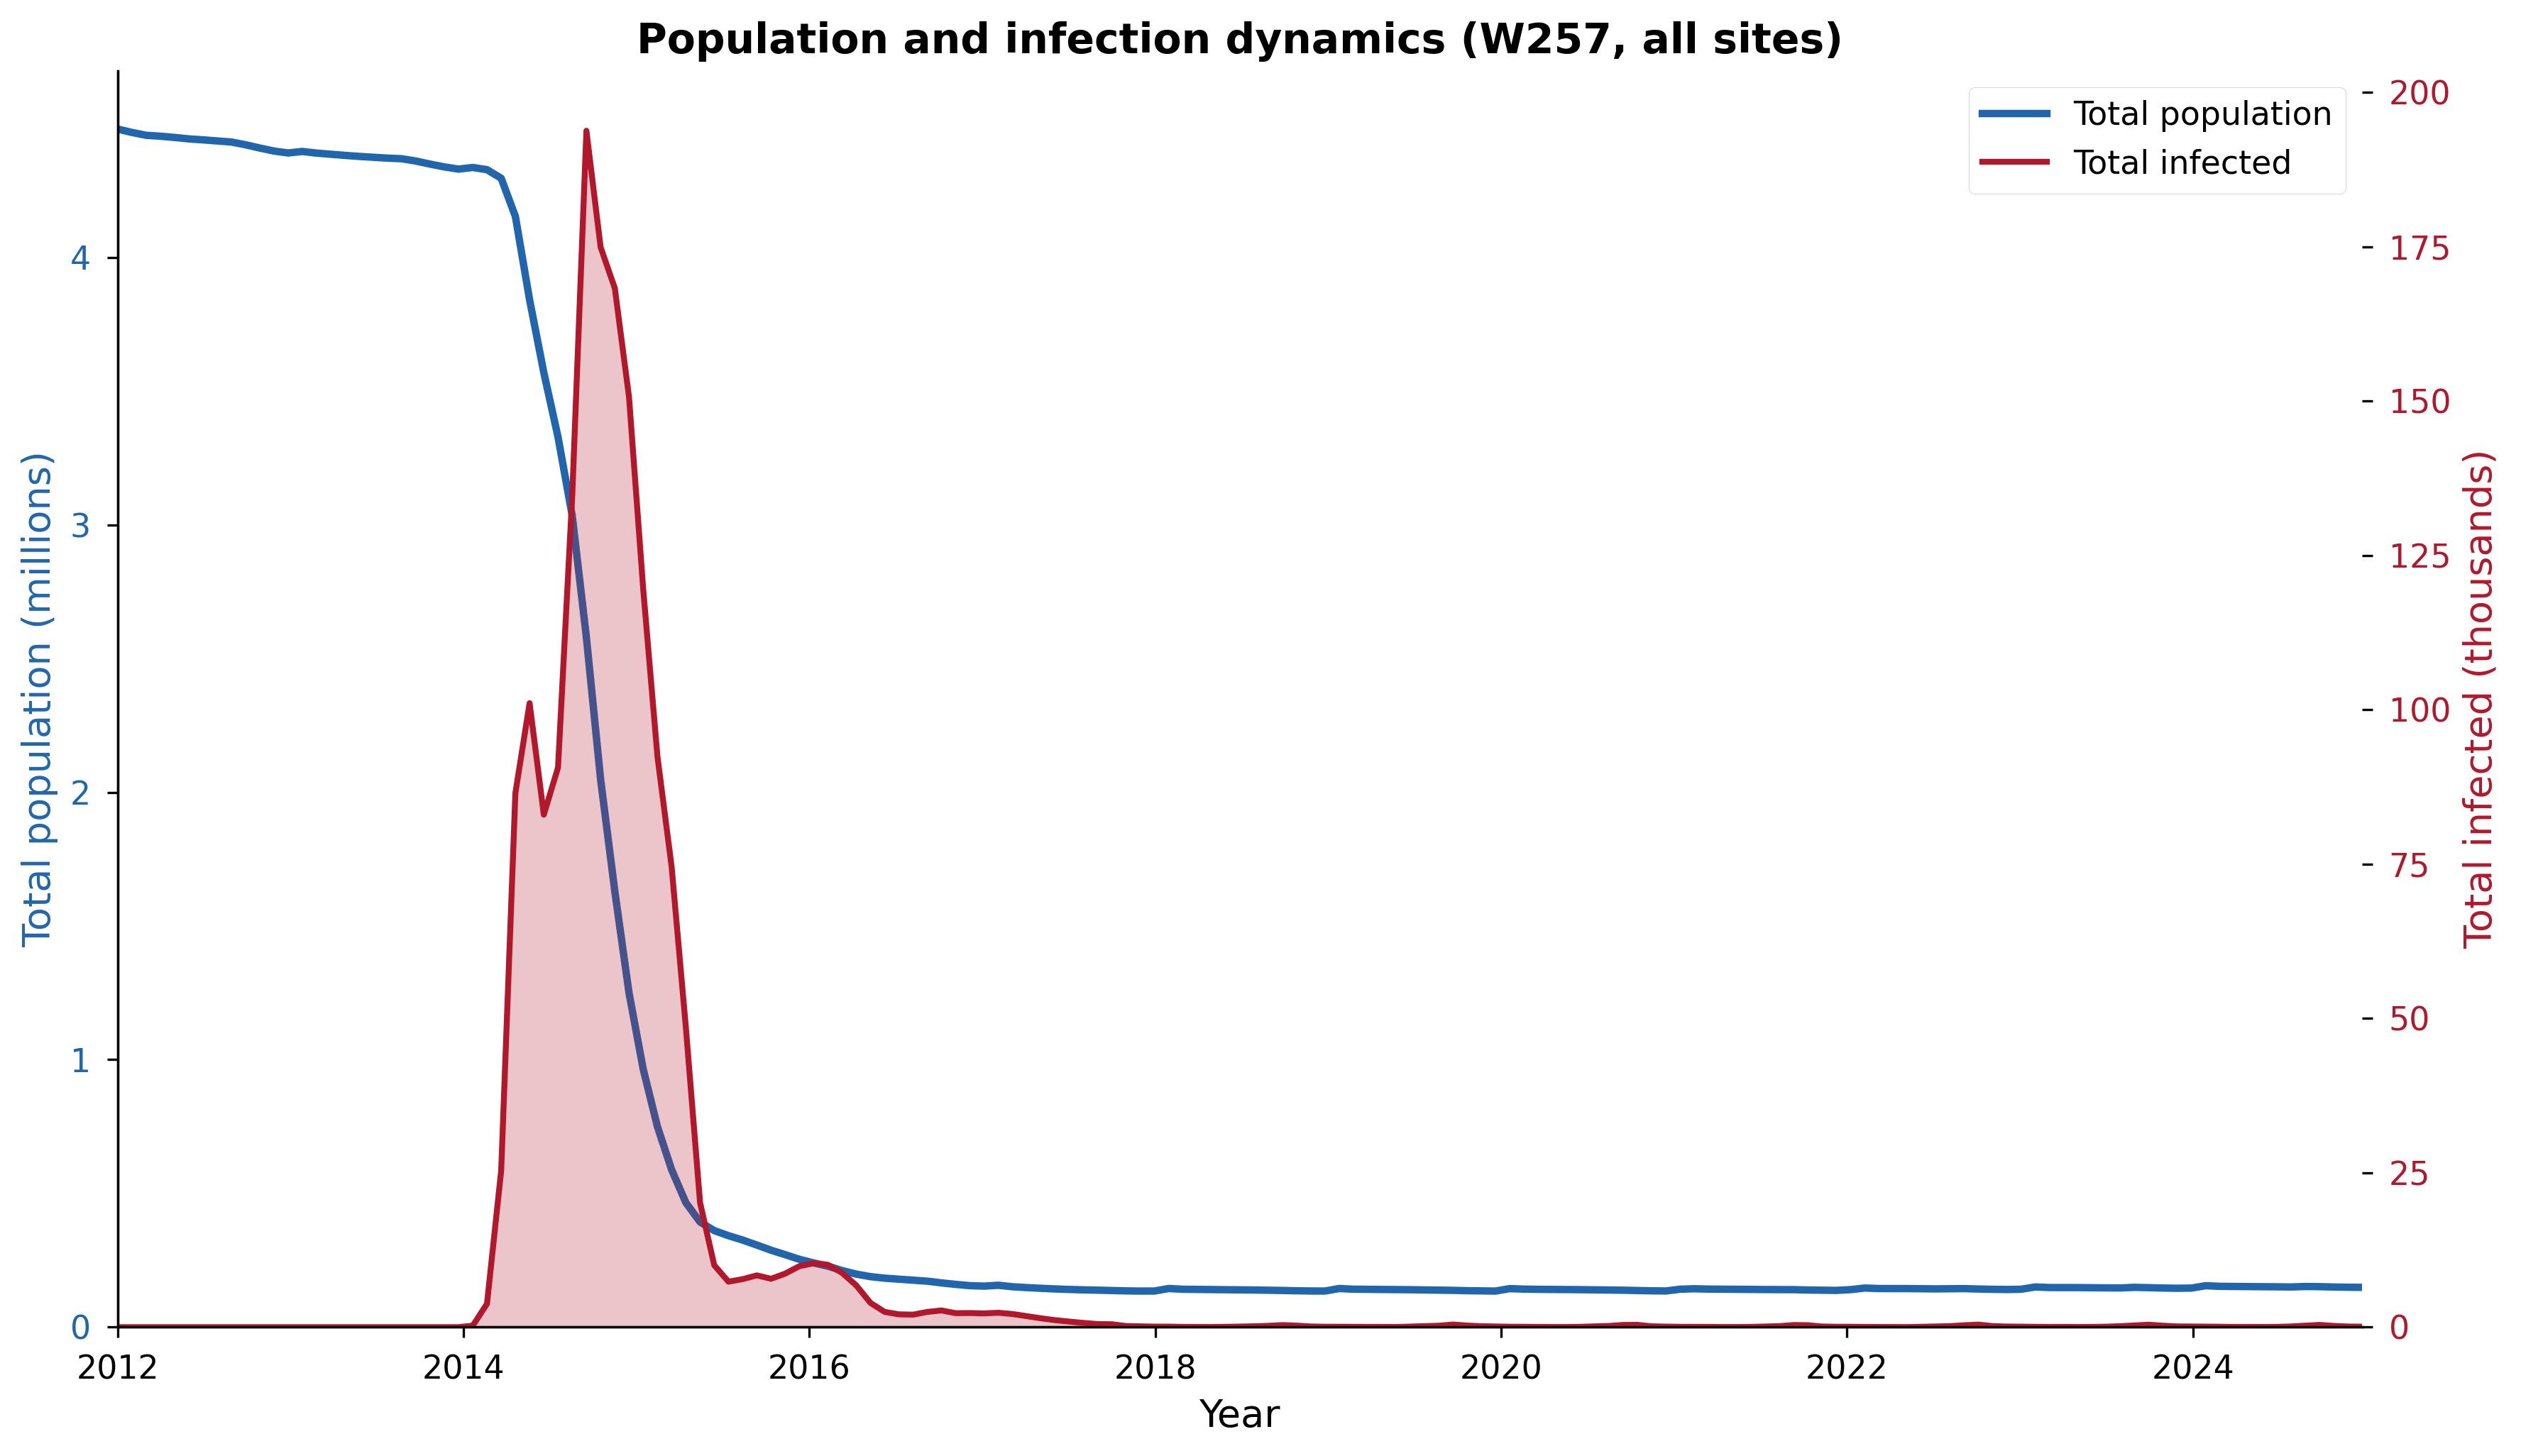
\includegraphics[width=\textwidth]{figures/fig_st_pop_infection_overlay.png}
\caption{\textbf{Total population and infection dynamics (W257).} Dual-axis time series showing total population across all 896 sites (blue, left axis) and total infected count (red, right axis). The infection pulse peaks early in the simulation, driving the population crash from $\sim$4.5 million to $\sim$150,000 individuals. The temporal offset between infection peak and population nadir reflects the delay between infection and mortality.}
\label{fig:st_pop_infection_overlay}
\end{figure}

\clearpage

\begin{figure}[H]
\centering
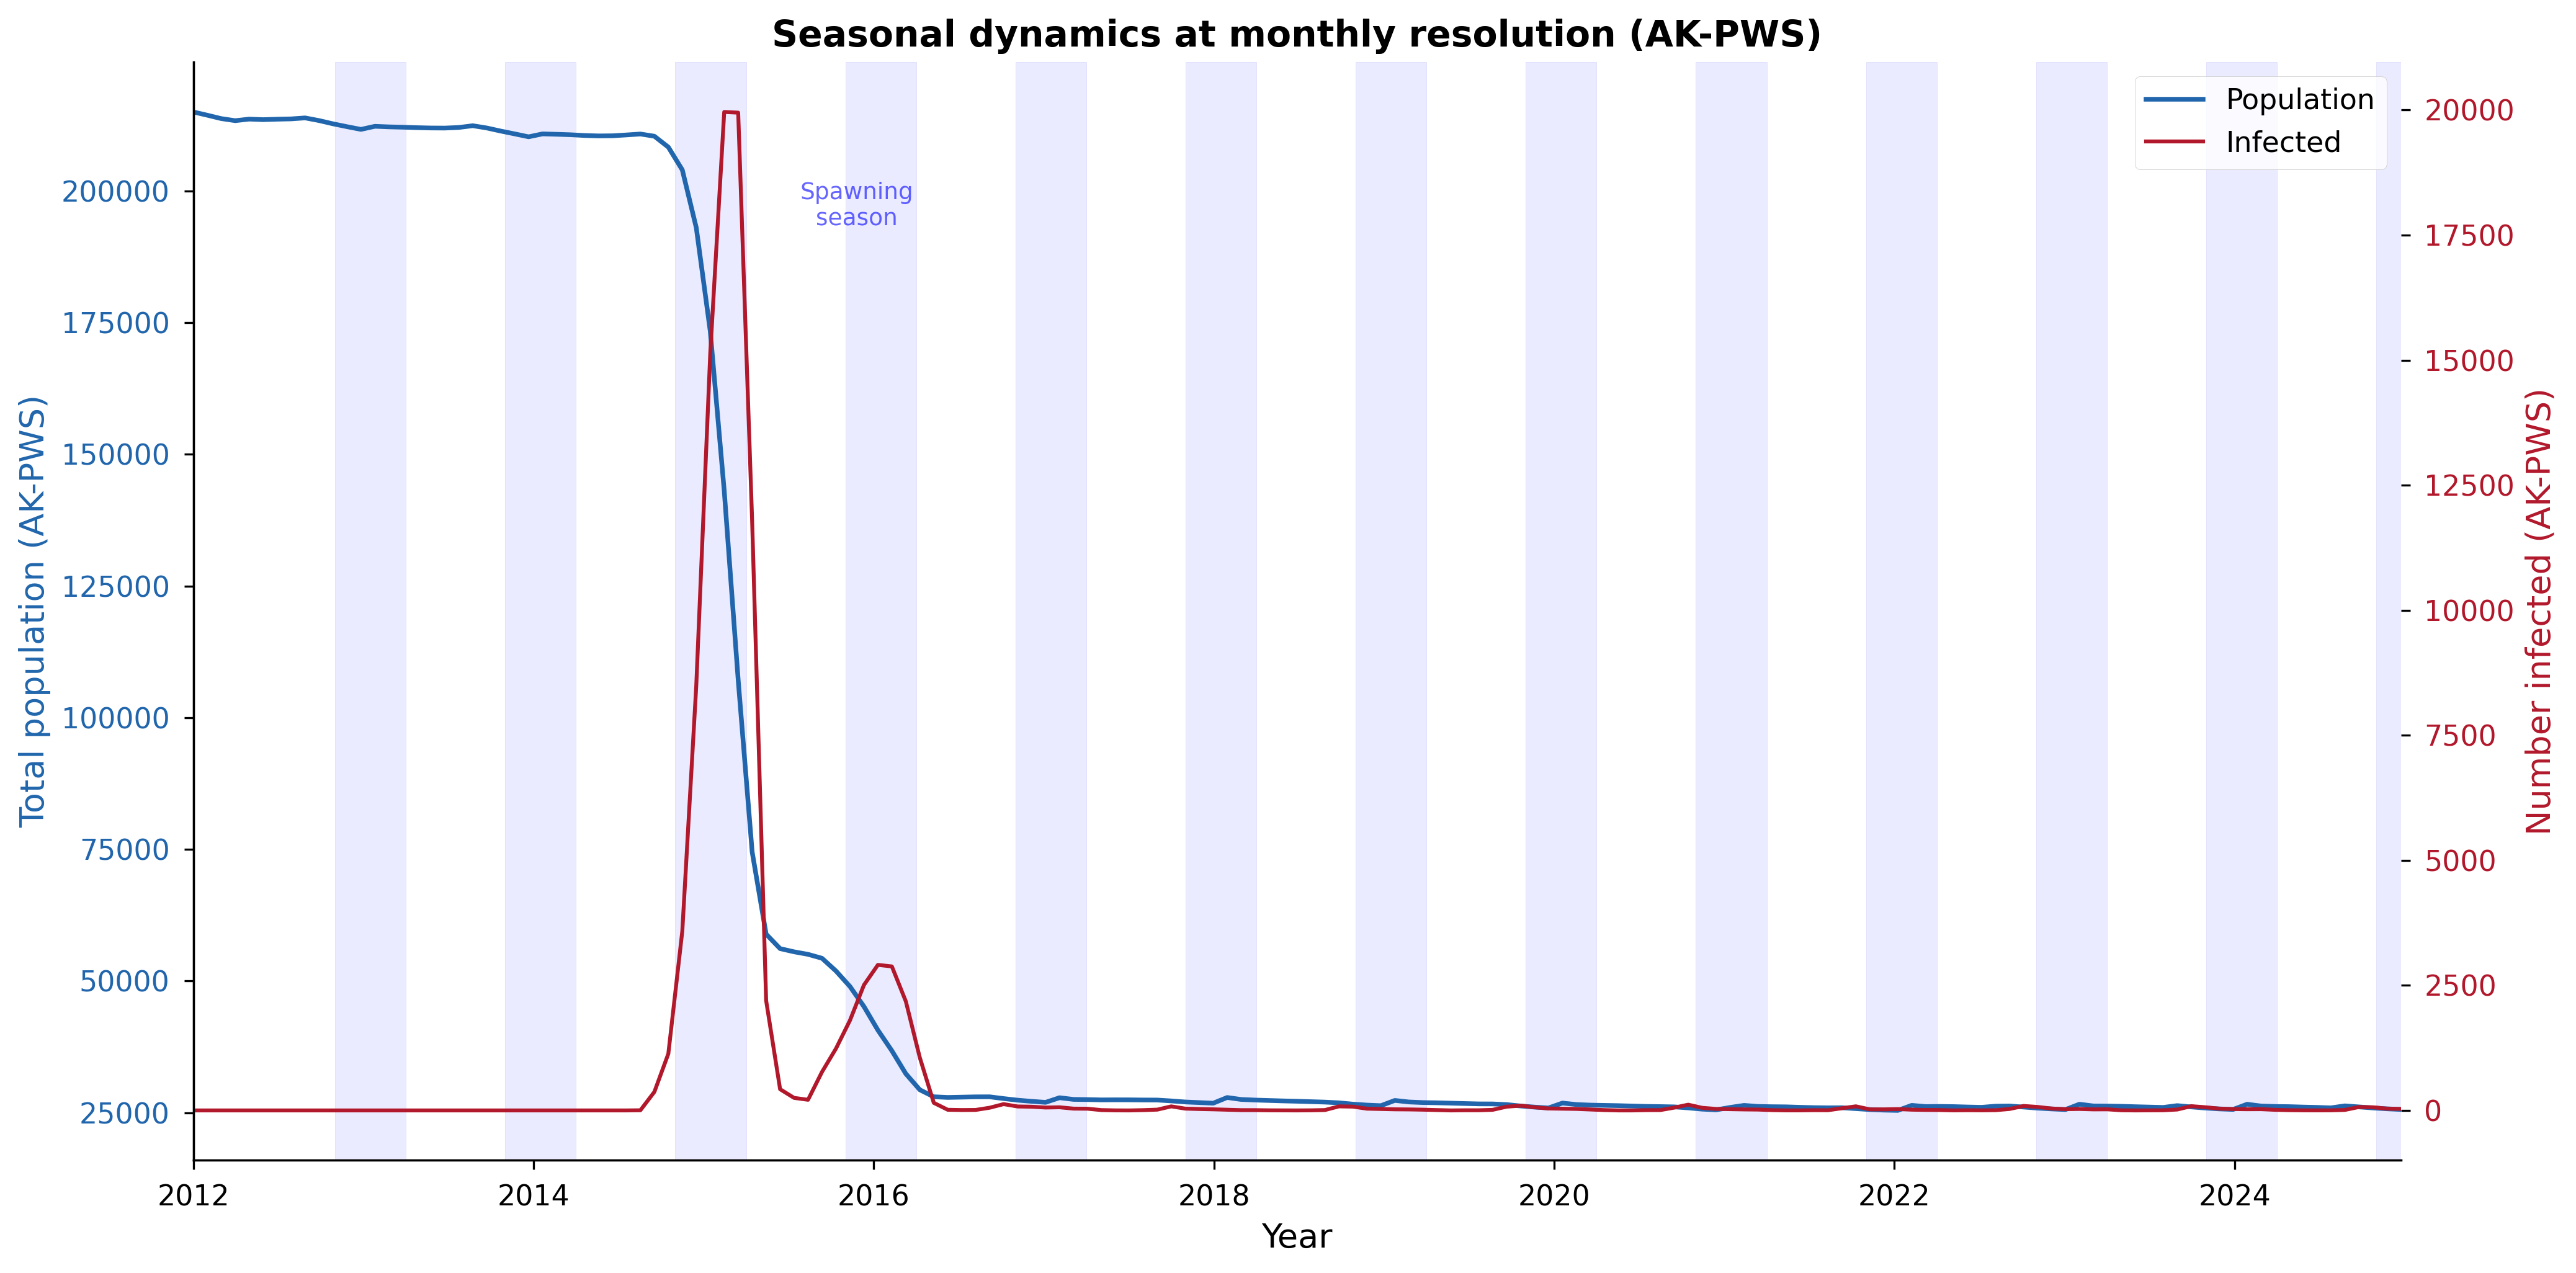
\includegraphics[width=\textwidth]{figures/fig_st_seasonal_dynamics.png}
\caption{\textbf{Seasonal dynamics in AK-PWS at monthly resolution.} Population (blue) and infection count (red) for the 43 AK-PWS sites. Monthly resolution reveals seasonal recruitment pulses visible as periodic population increases. The interaction between spawning-driven recovery and disease-driven mortality determines the net population trajectory in this key northern region.}
\label{fig:st_seasonal_dynamics}
\end{figure}

\clearpage

\begin{figure}[H]
\centering
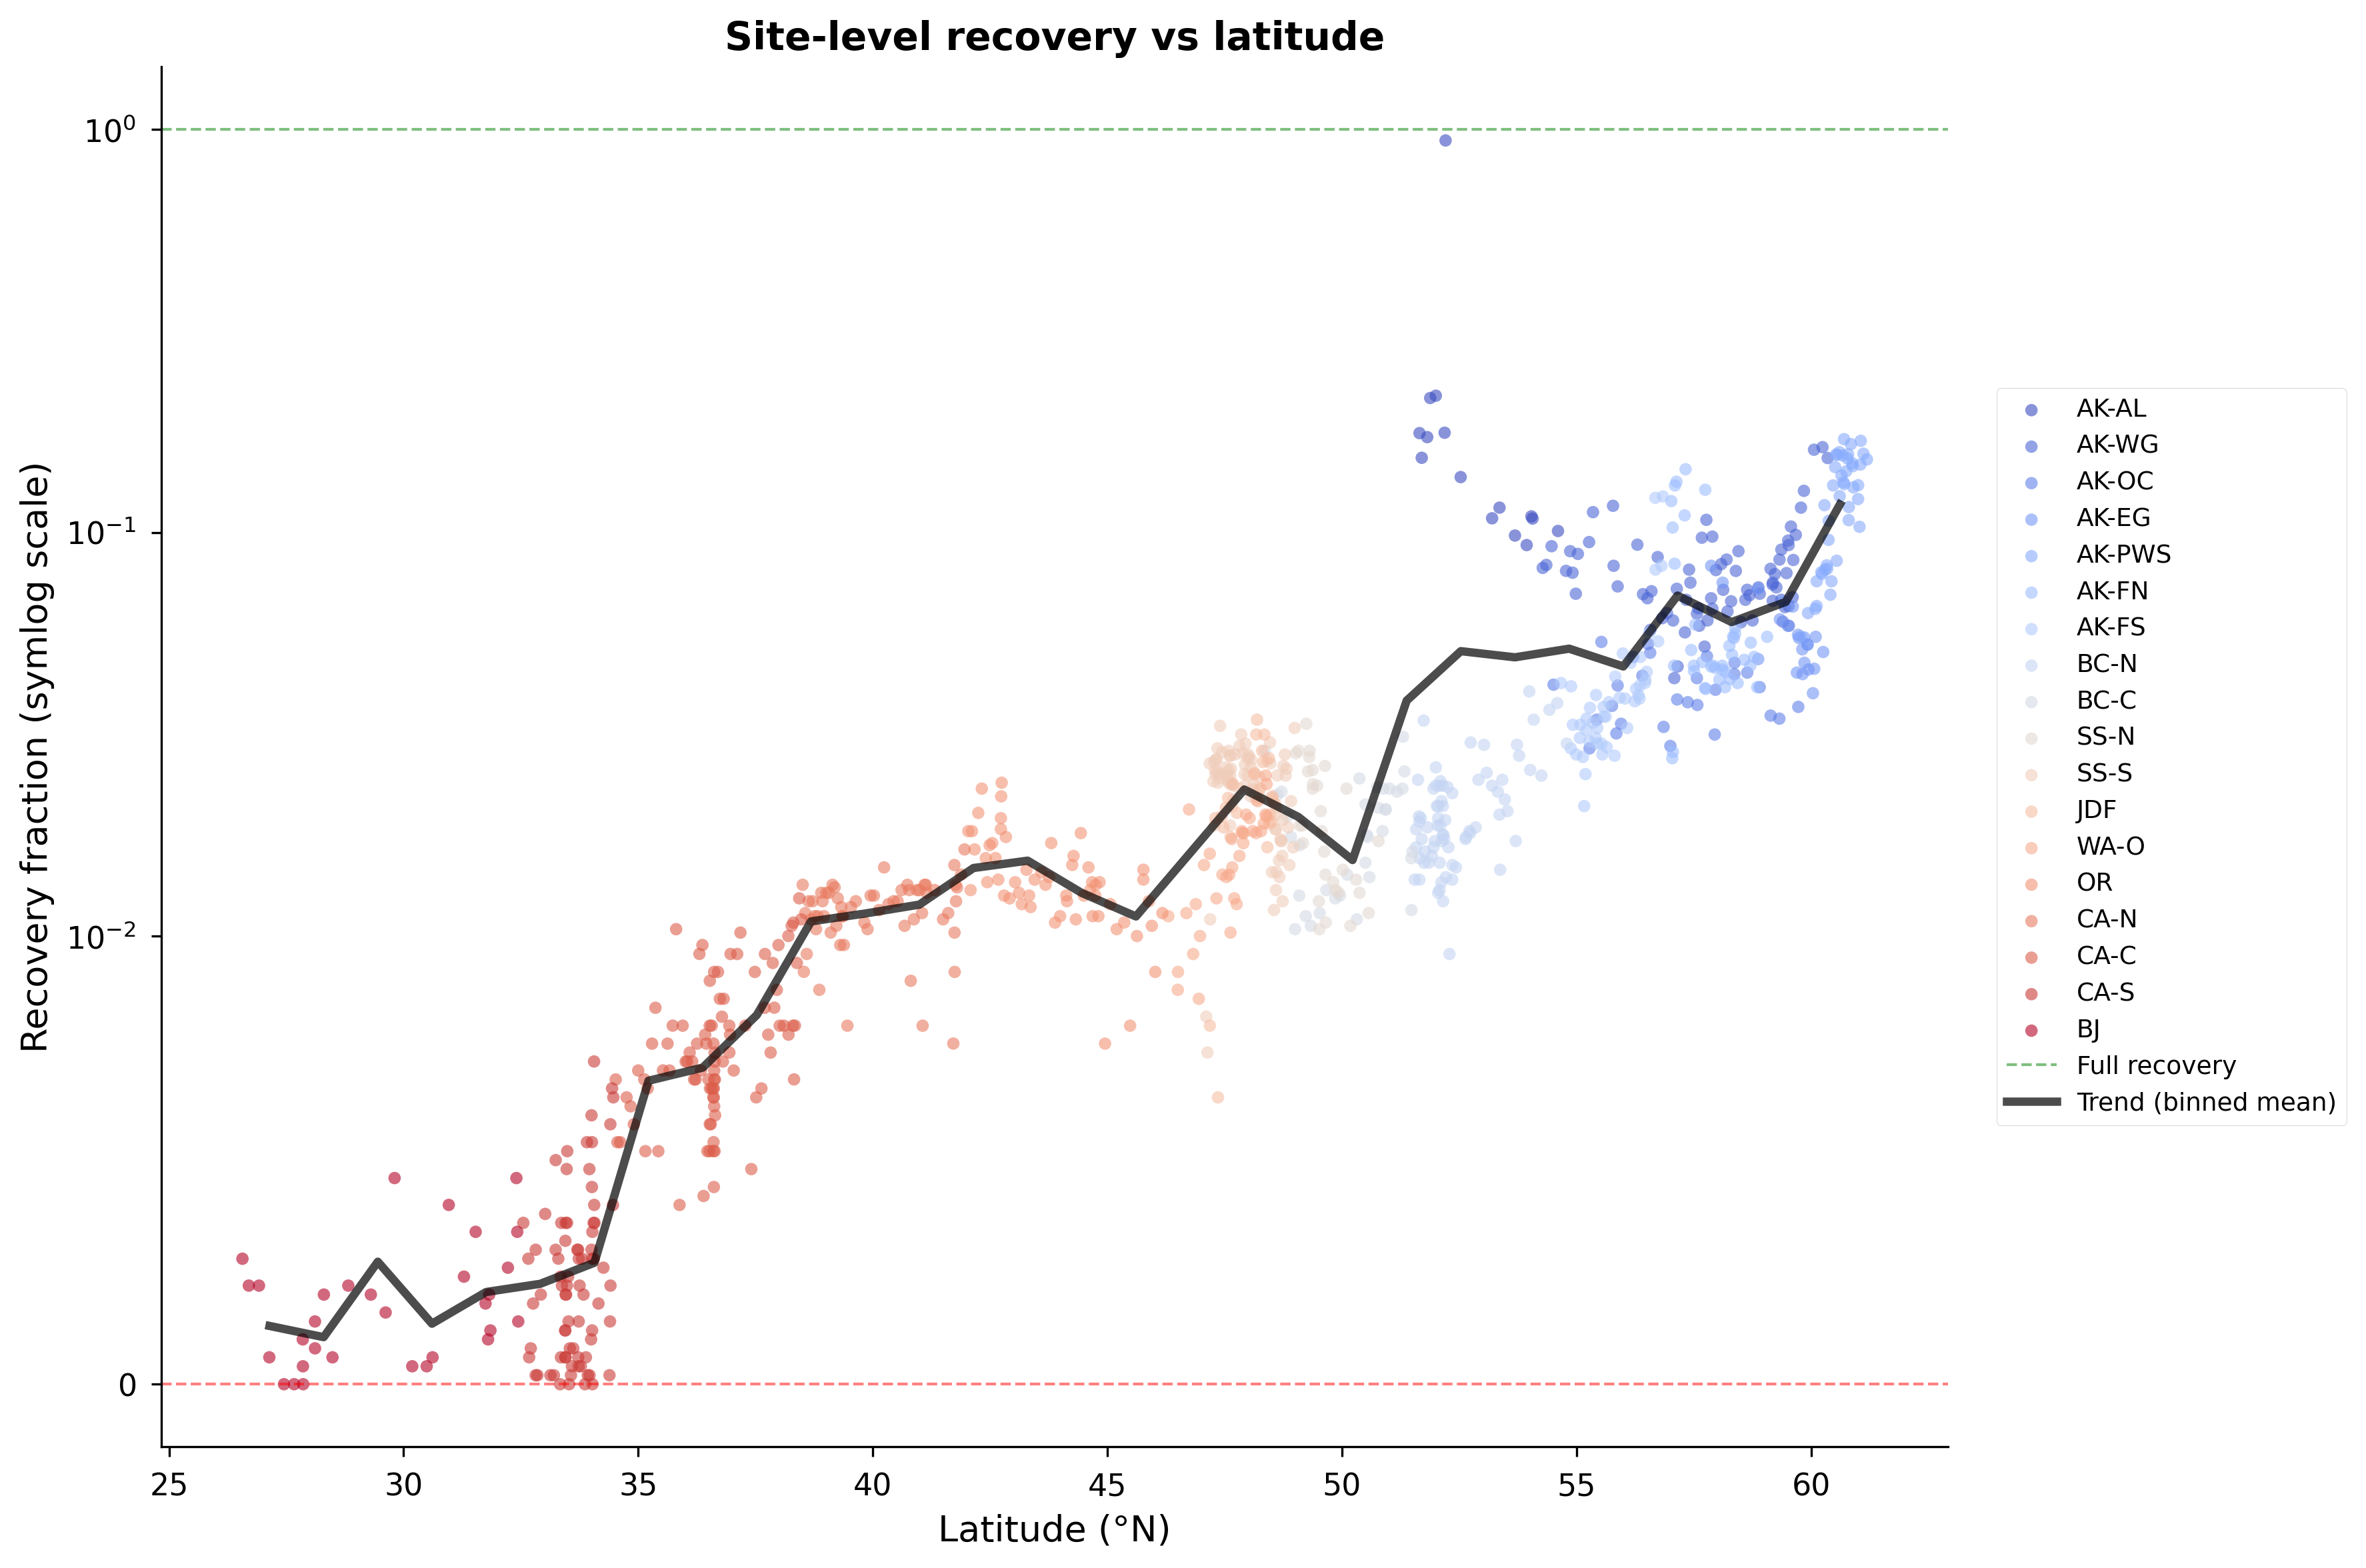
\includegraphics[width=\textwidth]{figures/fig_st_recovery_vs_latitude.png}
\caption{\textbf{Site-level recovery fraction versus latitude.} Each point represents one of 896 sites, colored by region. The strong positive relationship between latitude and recovery confirms the model's core spatial prediction: higher-latitude sites experience greater post-epidemic recovery. A trend line (LOESS smooth or moving average) highlights the gradient. The scatter around the trend reflects local site factors (flushing, connectivity, salinity).}
\label{fig:st_recovery_vs_latitude}
\end{figure}

\clearpage

% ══════════════════════════════════════════════════════════
% SECTION 5: TEMPORAL DYNAMICS
% ══════════════════════════════════════════════════════════
\section{Temporal Dynamics}

\sectionintro{Population and infection trajectories over the 13-year simulation. Monthly NPZ data reveals the timing and magnitude of epidemic impacts and recovery trajectories.}

\begin{figure}[H]
\centering
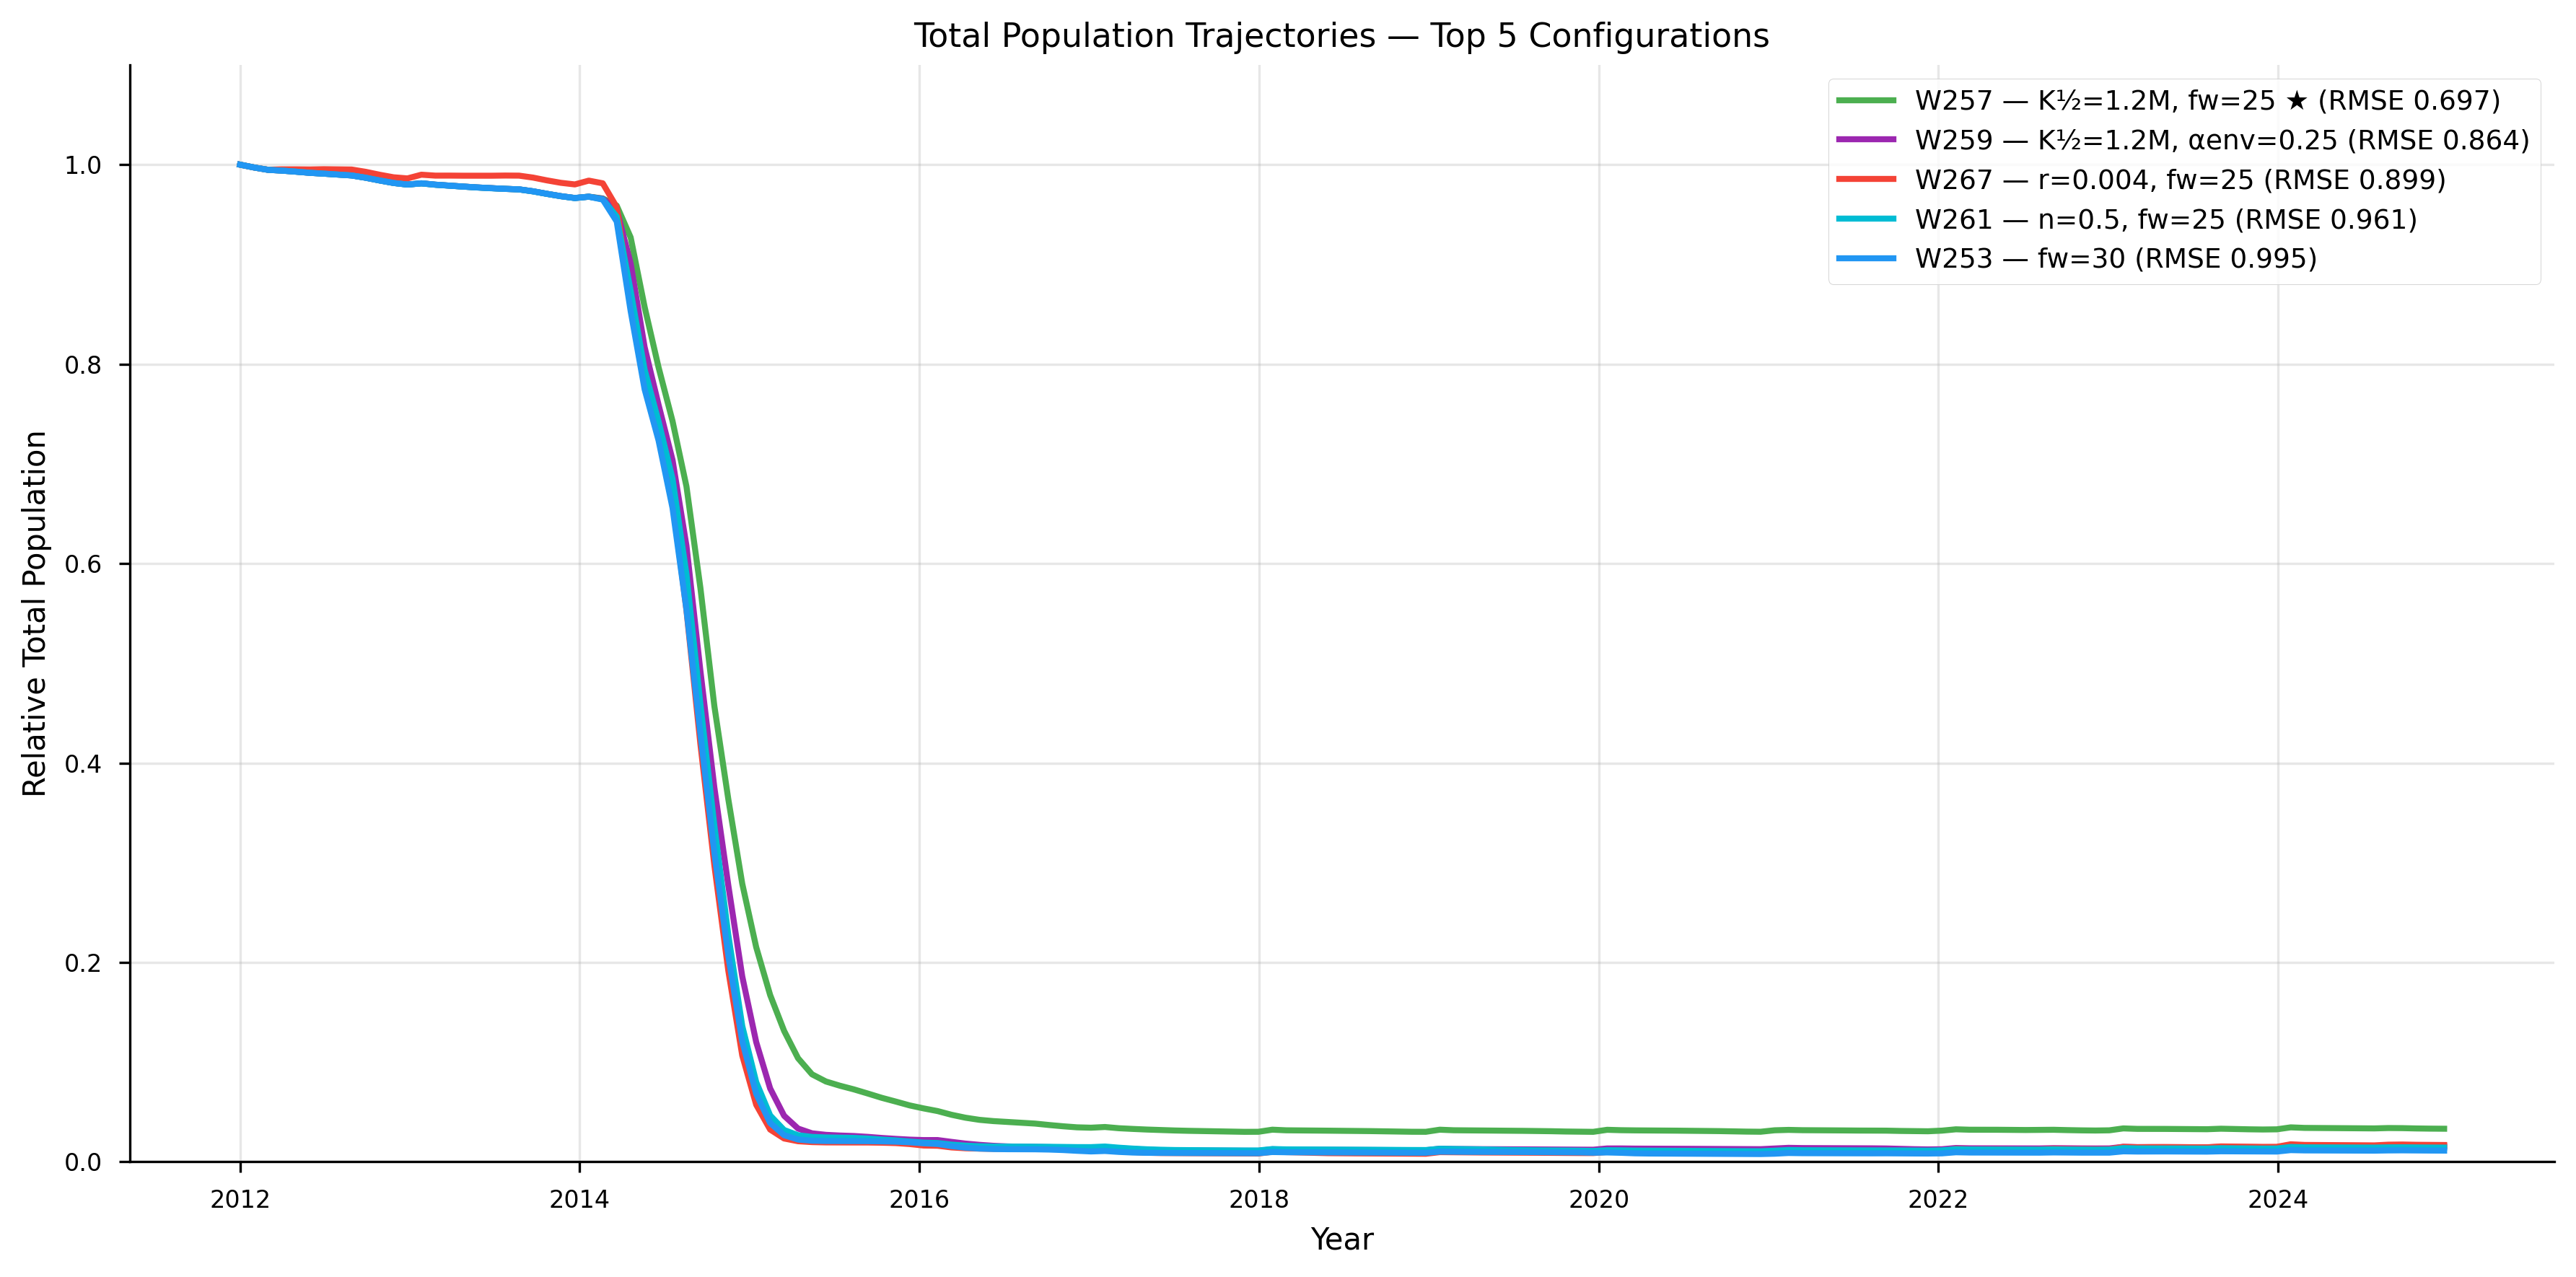
\includegraphics[width=\textwidth]{figures/fig_pop_trajectories_top5.png}
\caption{\textbf{Population trajectories for the top 5 configurations (W257, W259, W267, W261, W253).} Monthly total population over the 13-year simulation. All configurations show the 2013--2014 epidemic crash followed by partial recovery. W257 achieves the highest post-epidemic population, driven by $K_{\frac{1}{2}} = 1.2\text{M}$ enabling stronger density-dependent recruitment. The gap between W257 and W259 illustrates how $\alpha_{\text{env}} = 0.25$ suppresses late-stage recovery.}
\label{fig:pop_trajectories_top5}
\end{figure}

\clearpage

\begin{figure}[H]
\centering
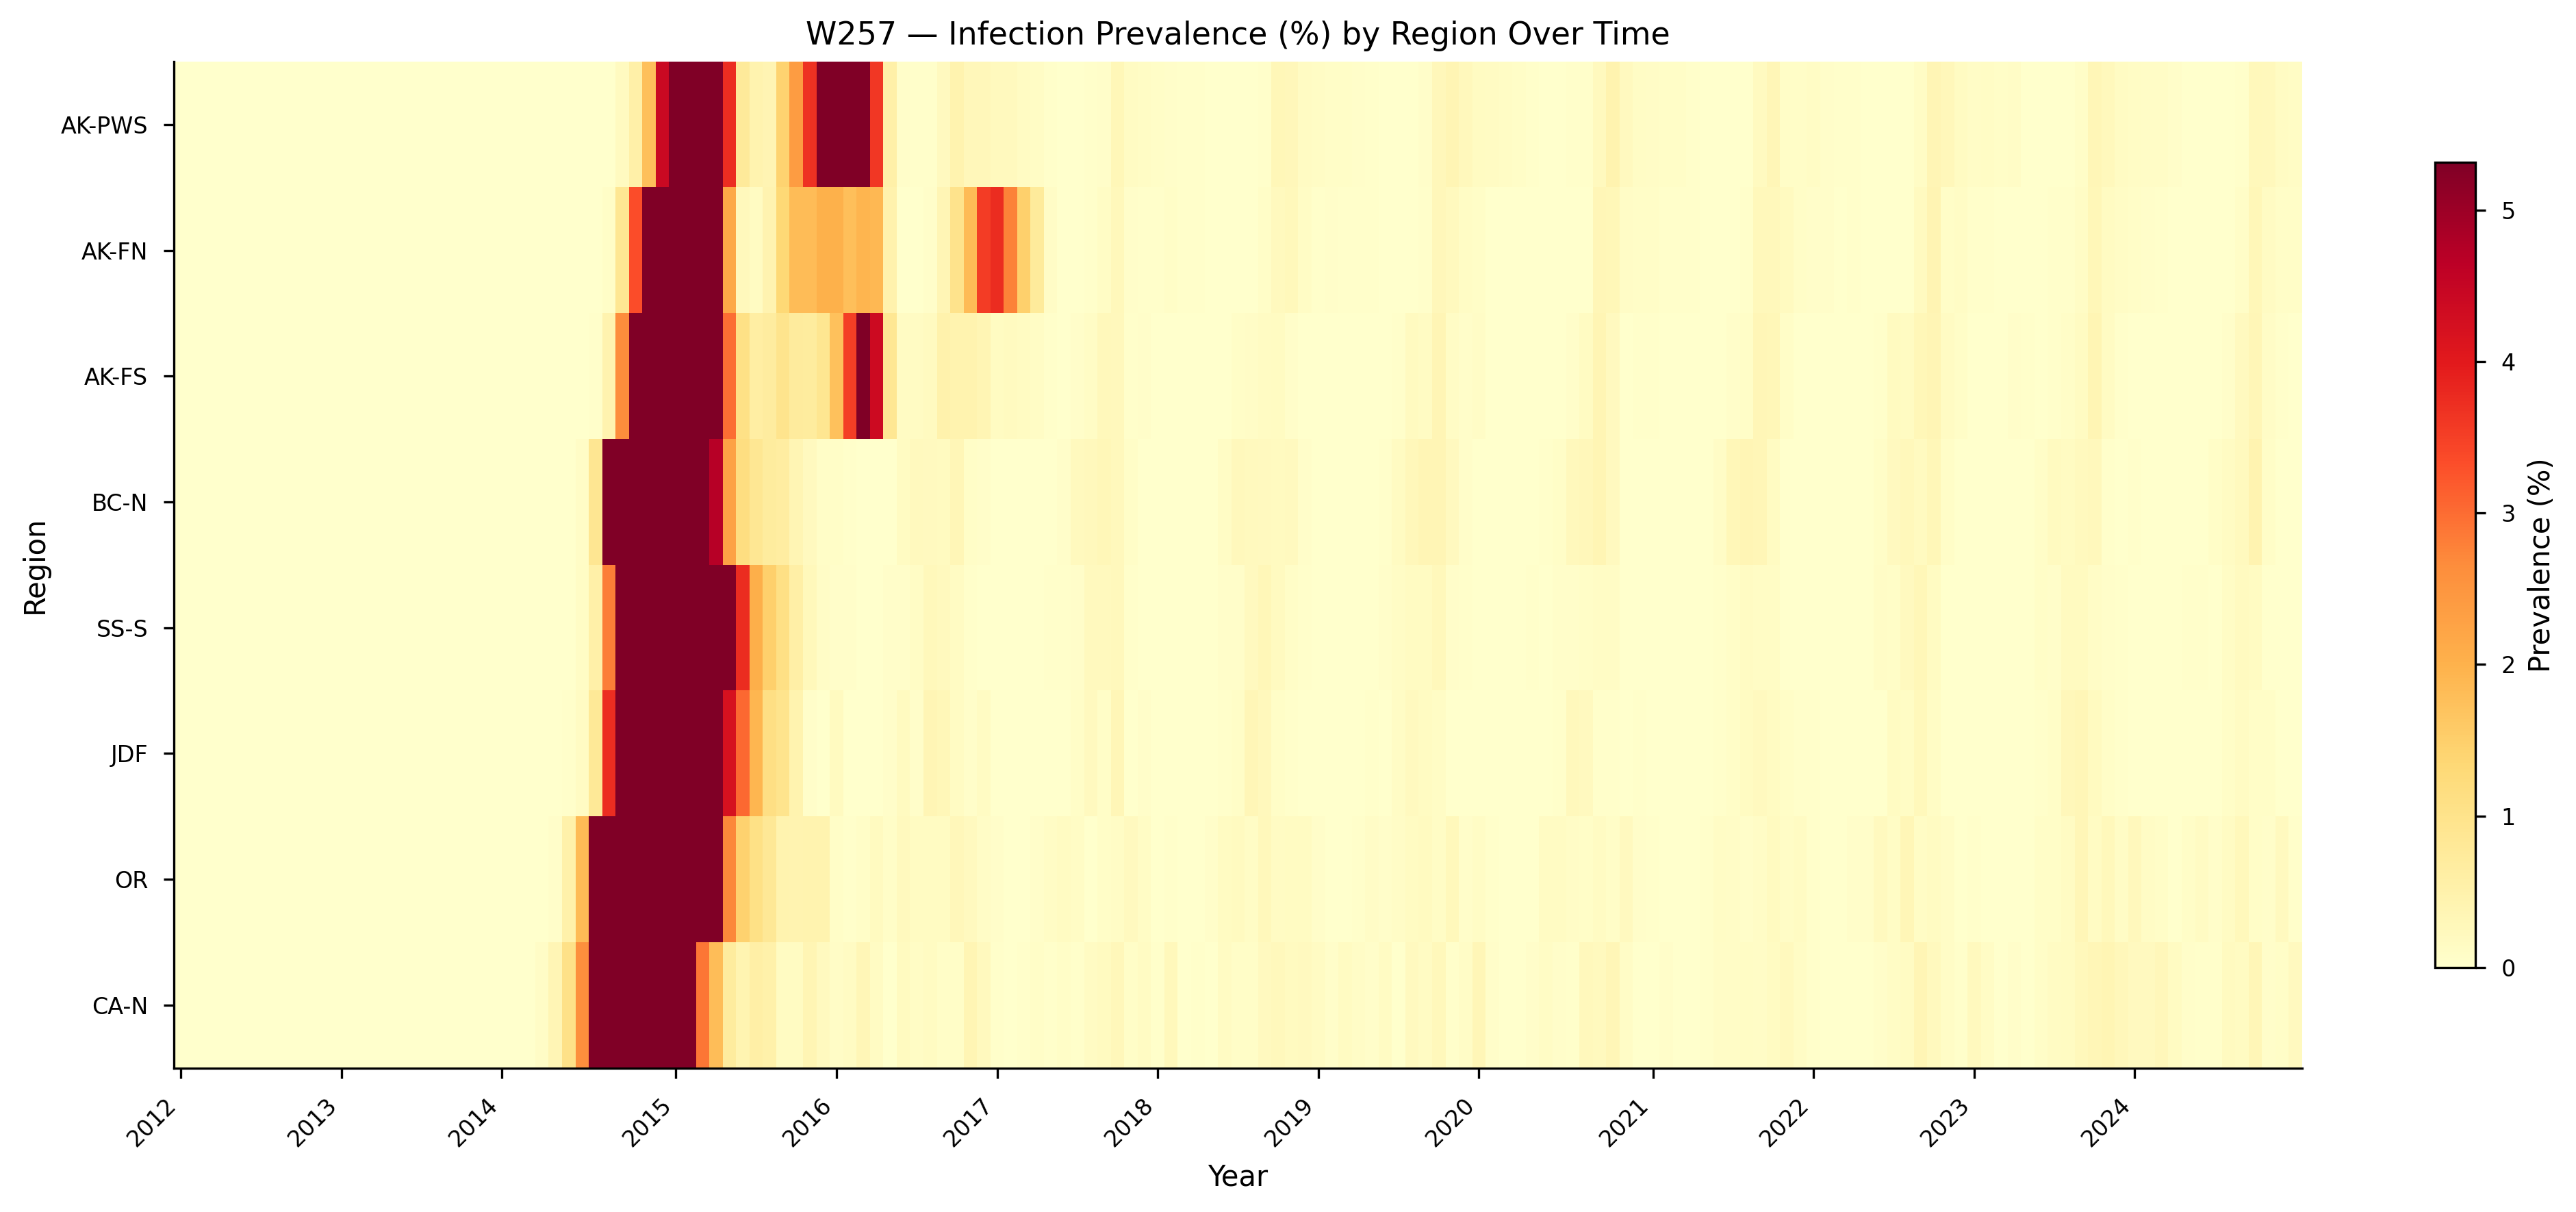
\includegraphics[width=\textwidth]{figures/fig_infection_heatmap.png}
\caption{\textbf{Infection prevalence heatmap for W257 ($K_{\frac{1}{2}} = 1.2\text{M}$, $f_w = 25$).} Time (months, $x$-axis) vs.\ region ($y$-axis); color intensity indicates fraction of population infected. The epidemic wave initiates in 2013, peaks across all regions, then declines as host resistance evolves. Alaska regions show sustained low-level infection post-peak, consistent with their higher recovery. Southern regions show rapid infection clearance but also near-complete population loss.}
\label{fig:infection_heatmap}
\end{figure}

\clearpage

\begin{figure}[H]
\centering
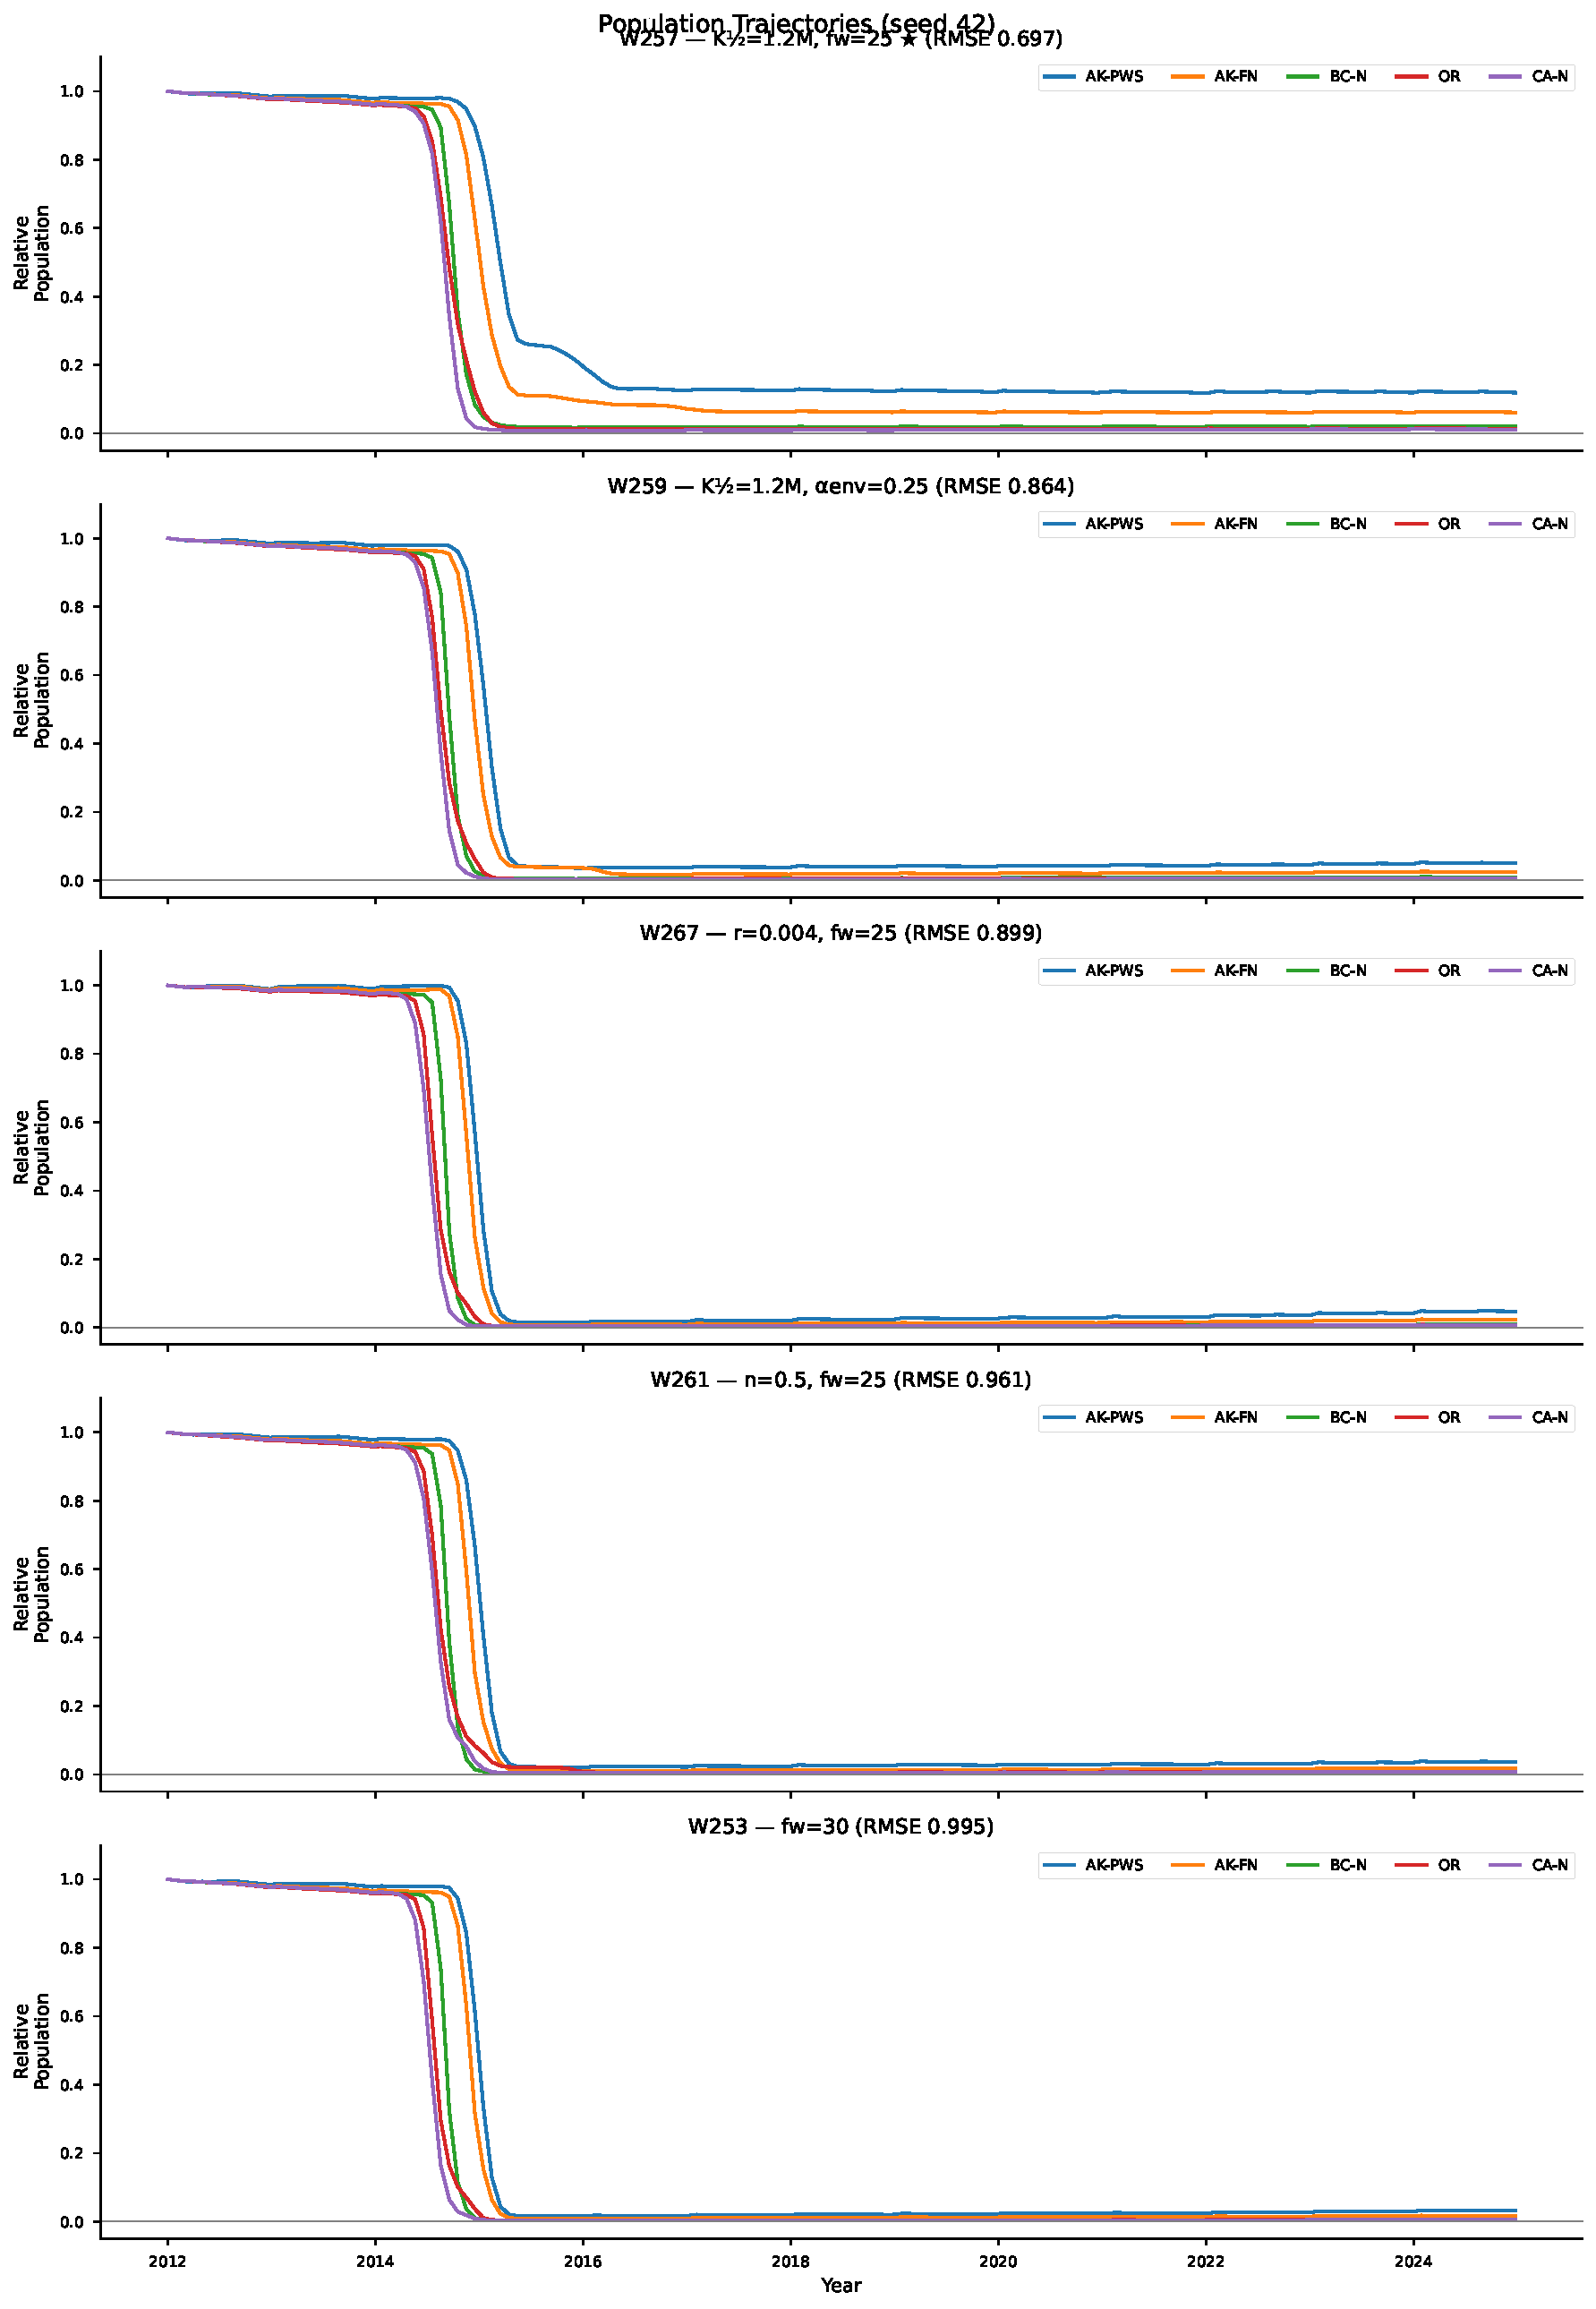
\includegraphics[width=\textwidth]{figures/fig_trajectories.pdf}
\caption{\textbf{Regional population time series from monthly NPZ data.} Multi-panel view showing population trajectories per region for top configurations. Unlike Figure~\ref{fig:pop_trajectories_top5} (which aggregates across regions), this figure reveals the per-region dynamics: Alaska regions (AK-PWS, AK-FN) show meaningful recovery in W257, while southern regions (CA-N, OR) remain near-extinct across all configurations, illustrating the latitude-dependent recovery pattern.}
\label{fig:trajectories}
\end{figure}

\clearpage

% ══════════════════════════════════════════════════════════
% SECTION 6: PARAMETER ANALYSIS
% ══════════════════════════════════════════════════════════
\section{Parameter Analysis}

\sectionintro{How do individual parameters and their interactions affect calibration quality? This section identifies the dominant levers and quantifies parameter importance.}

\begin{figure}[H]
\centering
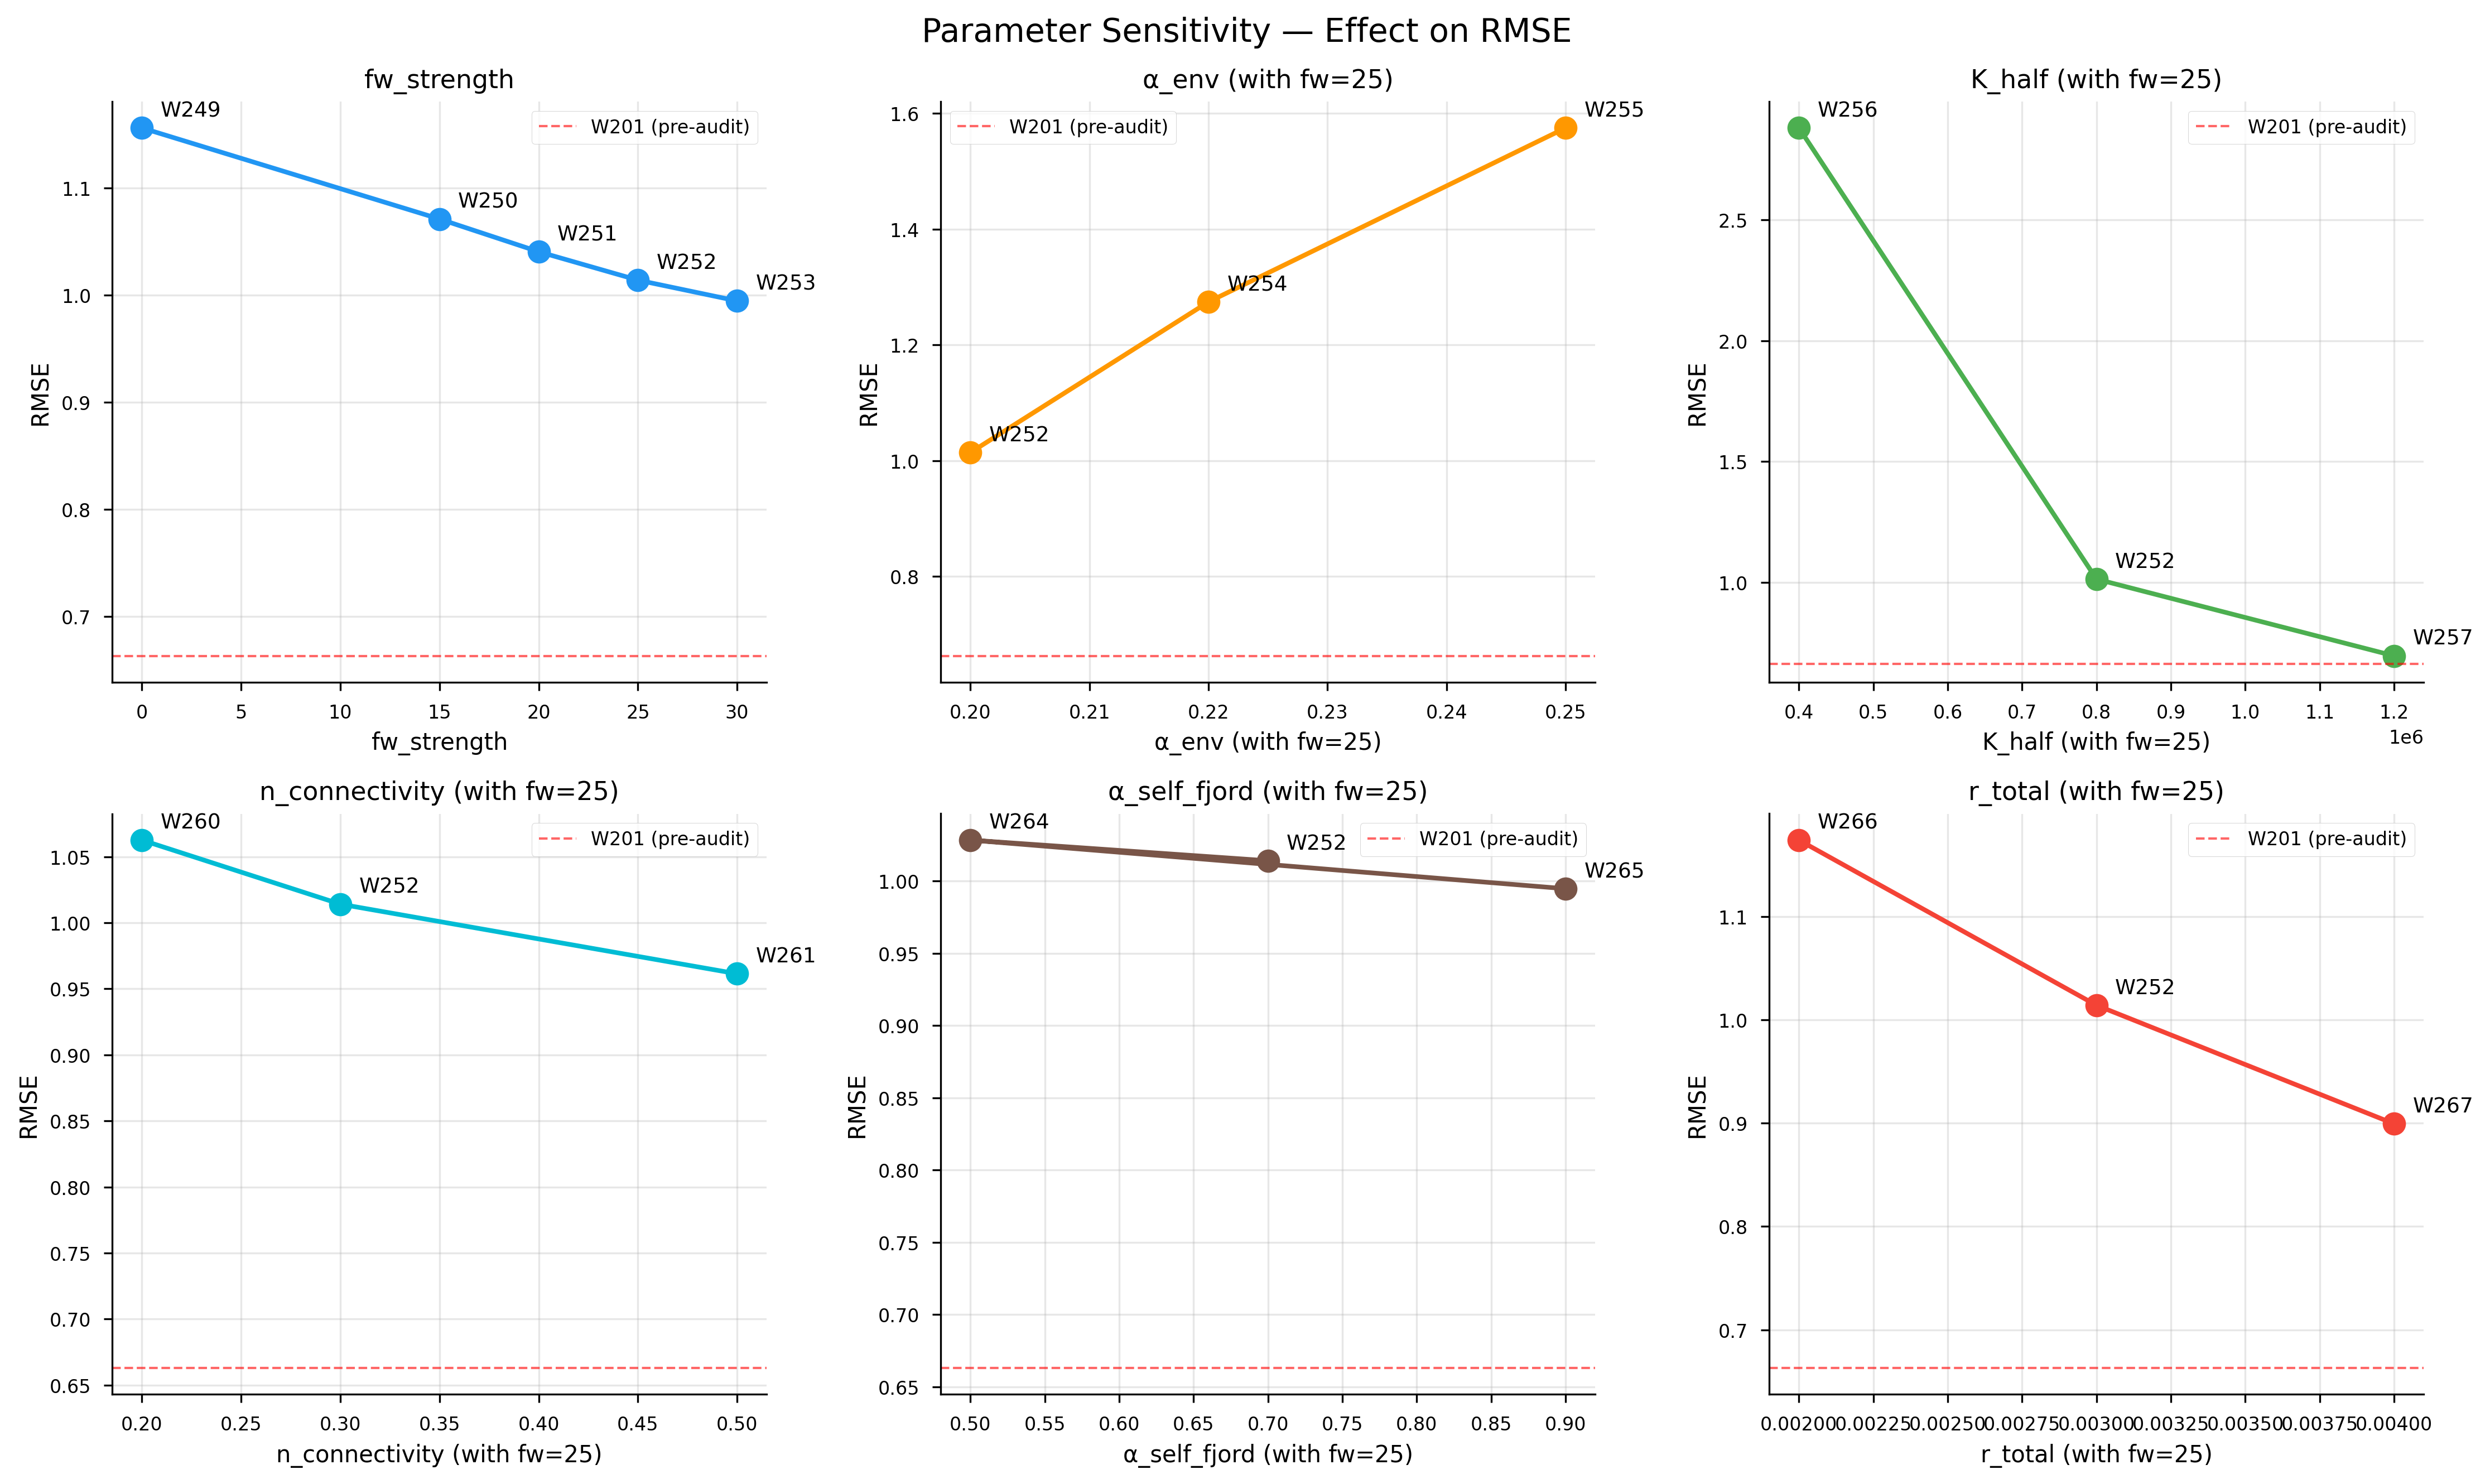
\includegraphics[width=\textwidth]{figures/fig_param_importance.png}
\caption{\textbf{Parameter importance analysis across six swept parameters.} Each panel shows the effect of one parameter on RMSE (left) and AK-PWS recovery (right). $K_{\frac{1}{2}}$ is the dominant lever: 400K $\to$ 1.2M shifts AK-PWS from $<$1\% to 12.1\% and RMSE from 2.88 to 0.70. The $f_w$ sweep (0--30) has a weaker monotonic effect (AK-PWS: 1.8\% $\to$ 3.2\%). $\alpha_{\text{env}} \geq 0.22$ is uniformly suppressive. Network connectivity and $r_{\text{total}}$ show intermediate effects.}
\label{fig:param_importance}
\end{figure}

\clearpage

\begin{figure}[H]
\centering
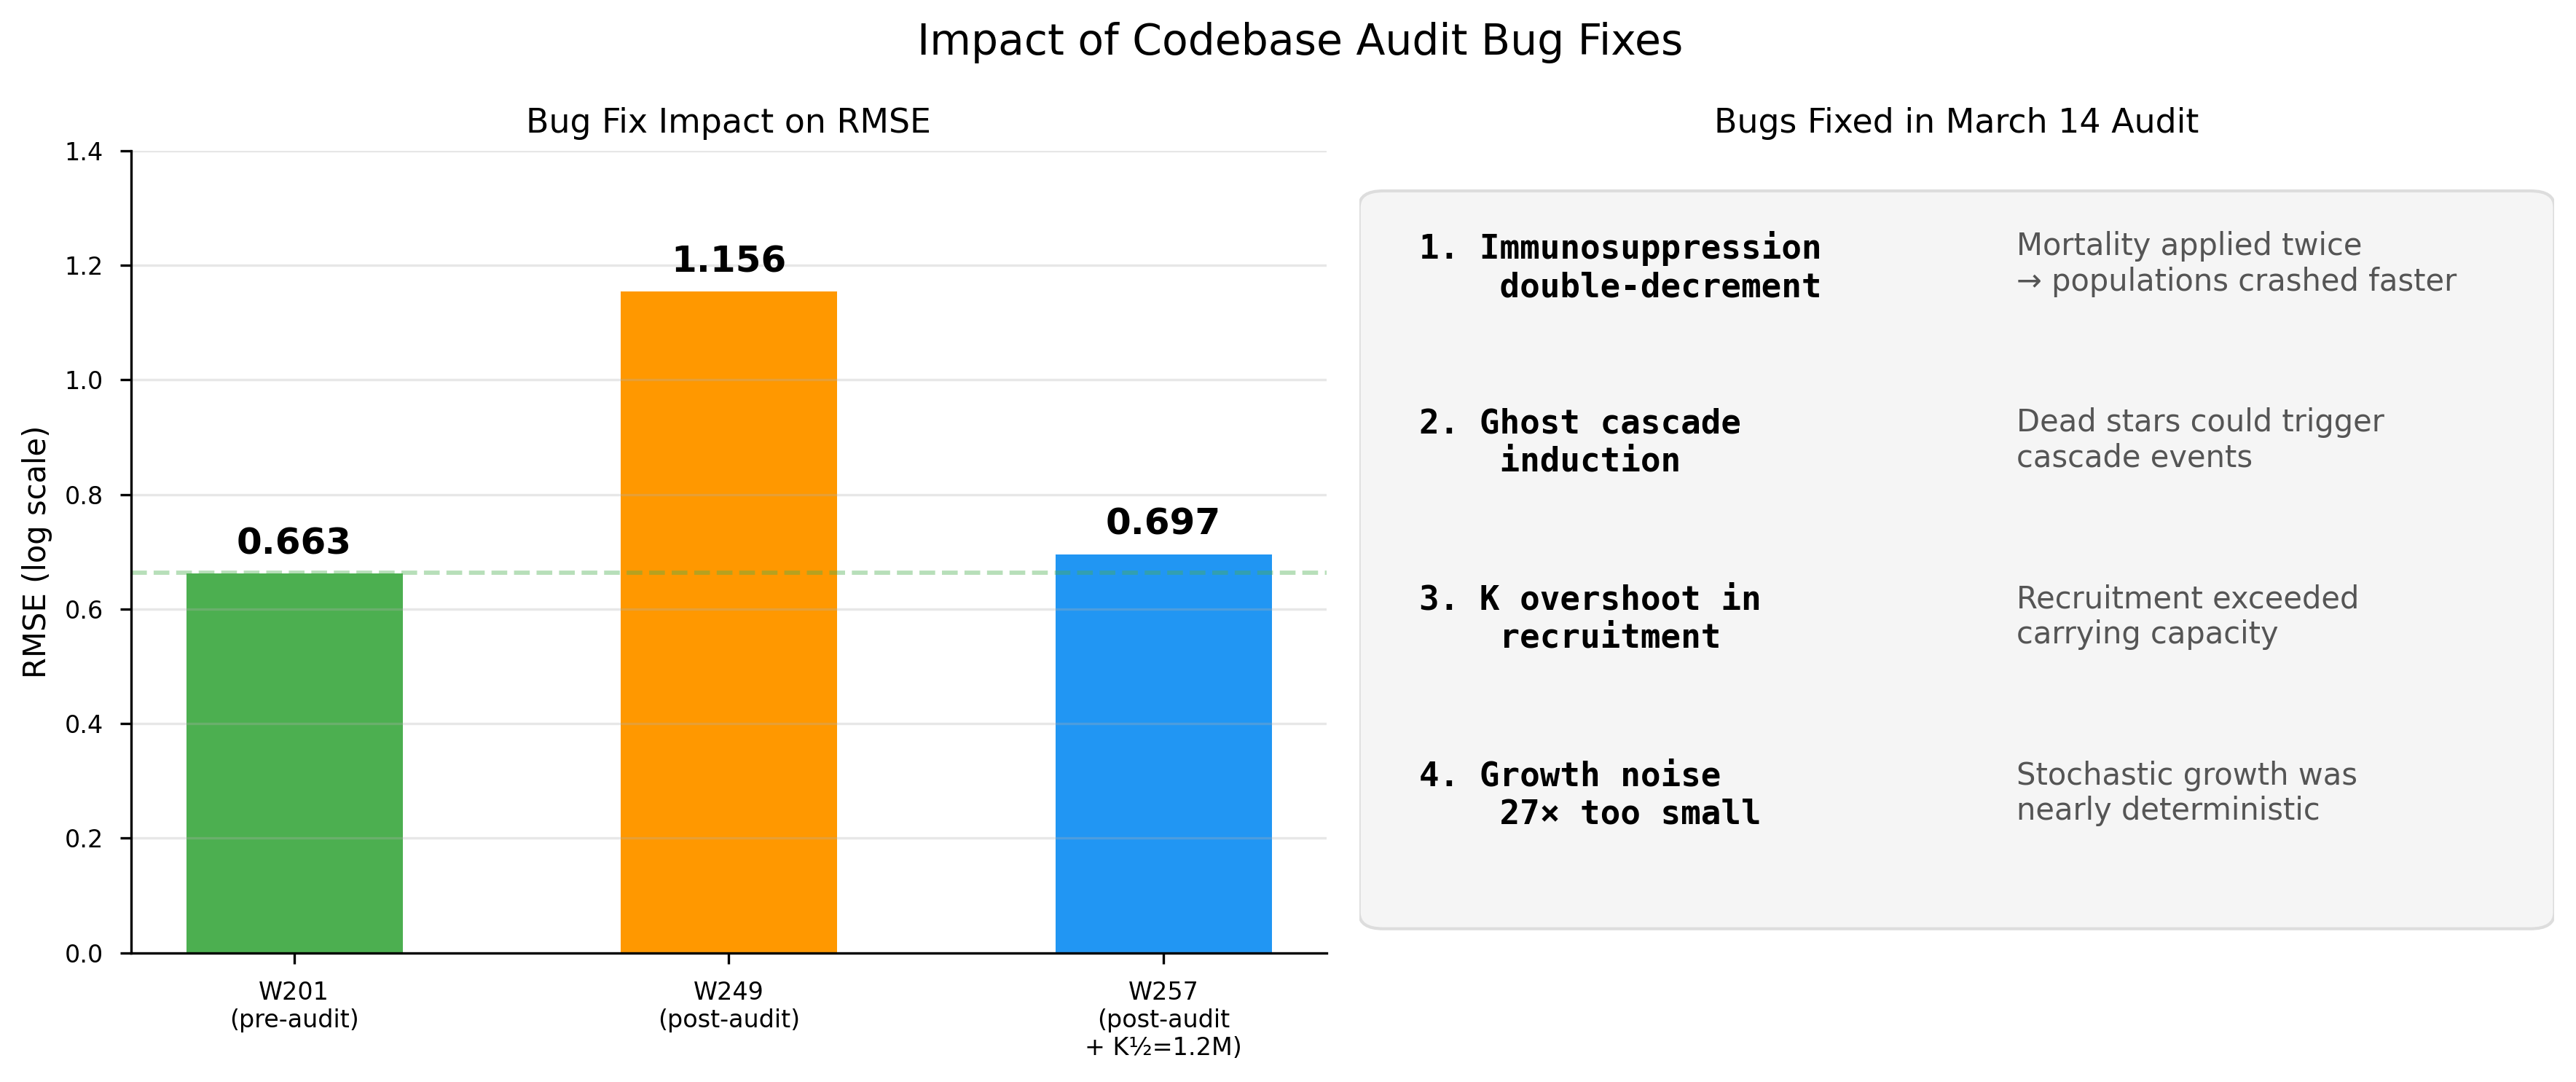
\includegraphics[width=\textwidth]{figures/fig_bug_fix_impact.png}
\caption{\textbf{Pre-audit vs.\ post-audit comparison.} The four March 14 bug fixes fundamentally altered model dynamics. The pre-audit W201 baseline achieved RMSE = 0.663, while the equivalent post-audit W249 baseline reaches only RMSE = 1.156 --- a 74\% degradation. This confirms that prior calibration is not transferable to the corrected codebase. However, W257 (RMSE = 0.697) nearly recovers the pre-audit performance level, demonstrating that $K_{\frac{1}{2}} = 1.2\text{M}$ compensates for the corrected dynamics.}
\label{fig:bug_fix_impact}
\end{figure}

\clearpage

% ══════════════════════════════════════════════════════════
% SECTION 7: CONCLUSIONS & NEXT STEPS
% ══════════════════════════════════════════════════════════
\section{Conclusions \& Next Steps}

\subsection{Key Findings}

\begin{enumerate}[nosep]
    \item \textbf{$K_{\frac{1}{2}}$ is the dominant lever.} Raising $K_{\frac{1}{2}}$ from 400K to 1.2M produces a $6\times$ improvement in AK-PWS recovery (from $<$1\% to 12.1\%) and a $4\times$ improvement in RMSE (from 2.88 to 0.70).
    \item \textbf{Post-audit calibration is viable.} Despite the four bug fixes degrading the baseline RMSE by 74\%, W257 recovers to within 5\% of the pre-audit best (0.697 vs.\ 0.663).
    \item \textbf{The latitude tradeoff persists.} CA-N overshoots its target by $12\times$ in the best configuration. Spatially uniform parameters cannot simultaneously achieve high Alaska recovery and low California recovery.
    \item \textbf{$\alpha_{\text{env}}$ is suppressive.} Environmental coupling at $\alpha_{\text{env}} \geq 0.22$ degrades RMSE substantially, reducing both northern and southern recovery.
\end{enumerate}

The 10 spatial-temporal visualizations (Section 4) demonstrate that the model reproduces the key qualitative features of the SSWD epidemic: southward-to-northward wavefront propagation, near-total crash across the range, and latitude-dependent partial recovery concentrated in Alaska.

\subsection{Recommended Next Steps}

\begin{enumerate}[nosep]
    \item \textbf{Fine-tune $K_{\frac{1}{2}}$} in the 0.8--1.5M range around the W257 optimum, with 3+ seeds for statistical confidence.
    \item \textbf{Add spatial modifiers} (latitude-dependent $K_{\frac{1}{2}}$ or region-specific $f_w$) to suppress southern overshooting while preserving Alaska recovery.
    \item \textbf{Investigate the $K_{\frac{1}{2}} \times \alpha_{\text{env}}$ interaction}: W259 shows that combining $K_{\frac{1}{2}} = 1.2\text{M}$ with $\alpha_{\text{env}} = 0.25$ reduces CA-N overshooting (0.64\% vs.\ 1.22\%) but also halves AK-PWS recovery (5.2\% vs.\ 12.1\%). An intermediate $\alpha_{\text{env}}$ value may offer a better tradeoff.
    \item \textbf{Multi-seed validation}: All results are from a single seed (42). Confirm W257's superiority across 3--5 seeds before committing to the $K_{\frac{1}{2}} = 1.2\text{M}$ regime.
\end{enumerate}

\clearpage

% ══════════════════════════════════════════════════════════
% APPENDIX: FULL METRICS TABLE
% ══════════════════════════════════════════════════════════
\appendix
\section{Full Metrics}
\label{app:metrics}

\begin{table}[H]
\centering
\footnotesize
\setlength{\tabcolsep}{3pt}
\begin{tabular}{ll r rrrrrrrr}
\toprule
\textbf{Rank} & \textbf{Config} & \textbf{RMSE} & \textbf{AK-PWS} & \textbf{AK-FN} & \textbf{AK-FS} & \textbf{BC-N} & \textbf{SS-S} & \textbf{JDF} & \textbf{OR} & \textbf{CA-N} \\
 & & & \textbf{(\%)} & \textbf{(\%)} & \textbf{(\%)} & \textbf{(\%)} & \textbf{(\%)} & \textbf{(\%)} & \textbf{(\%)} & \textbf{(\%)} \\
\midrule
& \textit{Target} & --- & \textit{30.0} & \textit{30.0} & \textit{20.0} & \textit{20.0} & \textit{5.0} & \textit{2.0} & \textit{0.25} & \textit{0.10} \\
\midrule
1  & \textbf{W257} & \textbf{0.697} & \textbf{12.11} & \textbf{6.27} & \textbf{4.32} & \textbf{2.12} & \textbf{2.36} & \textbf{2.25} & \textbf{1.45} & \textbf{1.22} \\
2  & W259 & 0.864 & 5.17 & 2.53 & 1.88 & 0.97 & 0.99 & 0.97 & 0.74 & 0.64 \\
3  & W267 & 0.899 & 4.77 & 2.31 & 1.89 & 0.84 & 0.95 & 0.94 & 0.78 & 0.76 \\
4  & W261 & 0.961 & 3.75 & 1.82 & 1.45 & 0.78 & 0.77 & 0.77 & 0.77 & 0.73 \\
5  & W253 & 0.995 & 3.20 & 1.71 & 1.41 & 0.54 & 0.64 & 0.63 & 0.54 & 0.50 \\
6  & W265 & 0.995 & 3.29 & 1.76 & 1.26 & 0.50 & 0.68 & 0.65 & 0.47 & 0.42 \\
7  & W252 & 1.014 & 2.91 & 1.55 & 1.27 & 0.54 & 0.58 & 0.58 & 0.50 & 0.41 \\
8  & W264 & 1.028 & 3.20 & 1.39 & 1.14 & 0.51 & 0.64 & 0.55 & 0.49 & 0.48 \\
9  & W251 & 1.041 & 2.83 & 1.34 & 1.10 & 0.51 & 0.61 & 0.56 & 0.52 & 0.46 \\
10 & W260 & 1.063 & 2.81 & 1.47 & 1.07 & 0.34 & 0.54 & 0.49 & 0.34 & 0.27 \\
11 & W250 & 1.071 & 2.49 & 1.22 & 0.97 & 0.47 & 0.57 & 0.59 & 0.53 & 0.46 \\
12 & W249 & 1.156 & 1.77 & 0.82 & 0.75 & 0.41 & 0.56 & 0.49 & 0.50 & 0.49 \\
13 & W266 & 1.174 & 1.94 & 1.15 & 0.71 & 0.29 & 0.35 & 0.36 & 0.31 & 0.28 \\
14 & W254 & 1.274 & 1.83 & 0.82 & 0.63 & 0.20 & 0.22 & 0.24 & 0.21 & 0.18 \\
15 & W263 & 1.407 & 1.40 & 0.55 & 0.41 & 0.15 & 0.15 & 0.16 & 0.31 & 0.24 \\
16 & W255 & 1.575 & 0.99 & 0.40 & 0.30 & 0.08 & 0.09 & 0.08 & 0.12 & 0.10 \\
17 & W262 & 1.690 & 0.89 & 0.33 & 0.30 & 0.04 & 0.08 & 0.06 & 0.05 & 0.04 \\
18 & W268 & 1.797 & 0.61 & 0.21 & 0.17 & 0.04 & 0.06 & 0.05 & 0.06 & 0.06 \\
19 & W256 & 2.879 & 0.08 & 0.02 & 0.02 & $<$0.01 & $<$0.01 & $<$0.01 & 0.01 & $<$0.01 \\
20 & W258 & 3.548 & 0.02 & 0.02 & $<$0.01 & $<$0.01 & $<$0.01 & 0.00 & $<$0.01 & $<$0.01 \\
\bottomrule
\end{tabular}
\caption{\textbf{Full metrics for all 20 configurations, ranked by RMSE.} Recovery values are shown as percentages for the 8 calibration regions. Target values are listed in the first data row for reference. W257 (bold) achieves the best overall RMSE and the highest recovery in all northern regions.}
\label{tab:full_metrics}
\end{table}

\end{document}
